\documentclass[12pt]{book}
\usepackage[utf8]{inputenc}
\usepackage[french, english]{babel}
\usepackage[T1]{fontenc}

\usepackage{amsfonts}
\usepackage{amsmath}
\usepackage{amssymb}
\usepackage{tikz}
\usepackage{graphicx}
\usepackage{color}
\usepackage{enumitem}
\usetikzlibrary{arrows}
\usepackage{framed}
\usepackage{arydshln}
\usepackage{multirow}
\usepackage{mathtools}
\usepackage{float}


% no indent
\setlength\parindent{0pt}

% theorems
\usepackage{amsthm}
\theoremstyle{definition}
\newtheorem{definition}{Definition}[section]
\newtheorem{proposition}{Proposition}[section]

\theoremstyle{remark}
\newtheorem{remark}{Remark}[section]

\theoremstyle{plain}


%comands
\newcommand{\bbr}{\mathbb{R}}
\newcommand{\bbt}{\mathbb{T}}
\newcommand{\bbv}{\mathbb{V}}
\newcommand{\bbn}{\mathbb{N}}

\newcommand{\cn}{\mathcal{N}}
\newcommand{\cl}{\mathcal{L}}

\newcommand{\todo}[1]{\textcolor{red}{TODO: #1\\}}

\begin{document}
\selectlanguage{english}

%
% Version info
%

Build version as of 2018-08-02 17:33:03
\newline
\input{revcount}
% \linenumbers


%
% Title
%

%\title{A Theory\\\begin{large}\emph{on}\end{large}\\Convolution of Graph Signals\\\begin{large}\emph{and its}\end{large}\\Application to Deep Learning}
\title{\begin{large}\emph{On}\end{large}\\Convolution of Graph Signals\\\begin{large}\emph{And}\end{large}\\Deep Learning on Graph Domains}
%\title{Convolution of Graph Signals\\and its Application to Deep Learning}
%\title{A Theory on Convolution of Graph Signals and its Application to Deep Learning}
\date{}
\maketitle

%
% Abstract
%

% will be included later
%
\begin{abstract}
\todo{after overview of chapter 2 is done ?}
\lipsum[1]
We build a theory of convolutions of graph signals, then we study and propose methods to extend neural networks to graph domains. Both problems are related since neural networks can make use of convolutions to leverage the underlying structure of the input domain.
\end{abstract}

%
% Table of contents
%

 \dominitoc
 \tableofcontents
 \adjustmtc

 % \listoffigures
 % \listoftables

%
% Introduction
%

\chapter*{Introduction}\label{chp:int}
\addcontentsline{toc}{chapter}{\nameref{chp:int}}

One of the first appearance of the \emph{convolution} was in the eighteenth century in D'Alembert's work \citep{wiki:enc}. Since then it has been used in a wide range of domains, including applied mathematics, physics, engineering, informatics and real world problems. In today's era of computerized industry and big data, the convolution has never been more useful. A famous example is its usage in deep learning algorithms for image processing \citep{lecun2015deep}. But this is just the tip of the iceberg. Years after years, IT companies aquire more and more data. With hashing algorithms, accessing single points or moderately sized batch of data is relatively easy. However, processing the entire database's knowledge is another story. Algorithms that don't scale well are too time consuming, so only those that traverse the entire database only a few times remain feasible. And that's the point: traversing the database (done in a parallelized manner) to process it can be modelized with a convolution. Therefore this little mathematical tool is bound to play a great role in our current and future civilizations ! % Now if we cut the bullshit and comeback down to earth, one 
A simple example can be seen in the company that funds this phd. One of its technology for processing large quantities of data is a programming language centered around a few frameworks. One of them %, that is called MAP\footnote{\url{http://www.warp10.io/reference/frameworks/framework-map/}} (in reference to another algorithm called MAP/REDUCE),
is nothing else than a reimplemention of the convolution by various complicated functions, which helps tremendously to produce simplified scripts.

%In this thesis work, our study is restricted to convolutions of graph signals and to deep learning models that can make use of it. This is a timely subject,

The subject of this thesis is a timely one, since deep learning have never received so much spotlight than in the last decade. However, deep learning models are often very specialized to their use cases. Standard Convolutional Neural Networks (CNNs) can only be applied to datasets for which each object can be modelized by a signal defined on an euclidean domain, like images or sounds. This is because the discrete convolution takes into account the structure of the domain of its inputs, in addition of their raw data. Our goal is to study and find ways to extend deep learning models to signals defined on a broader range of domains. To this end we build an algebraic theory of convolutions of graph signals, with the hope to characterize what a more generic definition of convolution should be and what properties should it preserve to keep its usefulness in deep learning models. We choose to modelize the domain of signals we study with a graph, since this structure can represent a wide range of domains. Our subject fits in the idea that efforts in the Artificial Intelligence (AI) field should tend toward a general-purpose AI, and in a lesser extent, that AI based algorithm, like deep learning, should seek genericity.

\begin{displayquote}
\begin{flushright}
\emph{The ultimate aim is to use these general-purpose technologies and apply them to all sorts of important real world problems.\\
--- Demis Hassabis}
\end{flushright}
\end{displayquote}

This manuscript is broke down in three chapters. Each chapter is preceded by a short overview so that the reader can grasp its essential developments at a glance. In \chapref{chap:1}, we present our domains of interest with a selected literature review. Then, in \chapref{chap:2}, we theorize an algebraic understanding of convolutions of graph signals. Finally, in \chapref{chap:3}, we study neural networks intended for graph domains.



%talk about graph == irregular

%
% Chapter 1
%

% cover
  \chapter{Presentation of the field}\label{chap:1}
  % \vfillIn this section, we present notions related to our domains of interest. In particular, for tensors we give original definitions that are more appropriate for our study. In the neural network's section, we present the concepts necessary to understand the evolution of the state of the art research in this field. In the last section, we present graphs for their usage in deep learning.

Vector spaces considered in what follows are assumed to be finite-dimensional and over the field of real numbers $\bbr$.\newpage
  % \vfill\minitoc\newpage
  \minitoc\newpage
  In this section, we present notions related to our domains of interest. In particular, for tensors we give original definitions that are more appropriate for our study. In the neural network's section, we present the concepts necessary to understand the evolution of the state of the art research in this field. In the last section, we present graphs for their usage in deep learning.

Vector spaces considered in what follows are assumed to be finite-dimensional and over the field of real numbers $\bbr$.\newpage

% body
  \subsection{Tensors}

Intuitively, tensors in the field of deep learning are defined as a generalization of vectors and matrices, as if vectors were tensors of rank $1$ and matrices were tensors of rank $2$. That is, they are objects in a linear space and their dimensions are indexed using as many indices as their rank, so that they can be represented by multidimensional arrays. In mathematics, a tensor is usually defined as a special class of multilinear functions. As such, a mathematical tensor is entirely defined on the cartesian product of the canonical bases onto which its outputs can be represented by a multidimensional array. In that sense, both definitions rejoin on their representation, but the underlying objects are different. In particular, mathematical tensors enjoy a more intrinsic definition as they neither depend on their multidimensional array representation nor on a change of basis.

Our definition of tensors is such that they are a bit more than multidimensional arrays but not as much as mathematical tensors, for that they are embedded in a linear space and any deep learning object can be later define rigorously.

\begin{definition}\textbf{Tensor space}\\
We define a \emph{tensor space} $\bbt$ of rank $r$ as a cartesian product of $r$ vector spaces under the coordinate-wise sum and the mono-linear outer product.

Its \emph{shape} is denoted $n_1 \times n_2 \times \cdots \times n_r$, where the $\{n_k\}$ are the dimensions of the vector spaces.
\end{definition}

Hence, a tensor space is a linear space. Note that for naming conveniency, we distinguish between the terms \emph{linear space} and \emph{vector space}. That is, we abusively use the term \emph{vector space} only to refer to a linear space that can be seen as a tensor space of rank $1$. If there is no notion of rank defined, we rather use the term \emph{linear space}.
We also make a clear distinction between the term \emph{dimension} (that is, for a tensor space it is equal to $\displaystyle \prod_{k=1}^r n_k$) and the term \emph{rank} (equal to $r$).

\begin{definition}\textbf{Tensor}\\
A \emph{tensor} $t$ is an object of a tensor space. The \emph{shape} of $t$, which is the same as the shape of the tensor space it belongs to, is denoted $n_1^{(t)} \times n_2^{(t)} \times \cdots \times n_r^{(t)}$.
\end{definition}

\begin{definition}\textbf{Indexing}\\
An \emph{entry} of a tensor $t$ is a scalar denoted $t[i_1, i_2, \ldots, i_r]$.

A \emph{subtensor} $t'$ is a tensor of same rank composed of entries of $t$ that are contiguous in the indexing, with at least one entry per rank. We denote $t' = t[l_1{:}u_1, l_2{:}u_2, \ldots, l_r{:}u_r]$, where the $\{l_p\}$ and the $\{u_p\}$ are the lower and upper bounds of the indices used by the entries that compose~$t'$.
\end{definition}

When using an index $i_k$ for an entry of a tensor $t$, we implicitly assume that $i_k \in \{1, 2, \cdots, n_k^{(t)}\}$ if nothing is precised.
For subtensor indexings, we don't necessarily write the lower bound index if it is equal to $1$, neither the upper bound index if it is equal to $n_p^{(t)}$.

\begin{definition}\textbf{Slicing}\\
A \emph{slice} operation, along the last ranks $\{r_1, r_2, \ldots, r_s\}$, and indexed by $(i_{r_1}, i_{r_2}, \ldots, i_{r_s})$, is a morphism $s: \bbt = \displaystyle \prod_{k=1}^r \bbv_k \rightarrow \prod_{k=1}^{r-s} \bbv_k$, such that:
\begin{align*}
s(t)[i'_1, i'_2, \ldots, i'_{r-s}] &= t[i'_1, i'_2, \ldots, i'_{r-s}, i_{r_1}, i_{r_2}, \ldots, i_{r_s}] \\
\text{ i.e. } \quad s(t) :&= t[:,:, \ldots, :, i_{r_1}, i_{r_2}, \ldots, i_{r_s}]
\end{align*}
where $:=$ means that values of the right operand are assigned to the left operand.
We denote $t_{i_{r_1}, i_{r_2}, \ldots i_{r_s}}$ and call it the \emph{slice} of $t$. 
Slicing along a subset of ranks that are not the lasts is defined similarly.
$s(\bbt)$ is called a \emph{sliced subspace}.
\end{definition}

\begin{definition}\textbf{Flattening}\\
A \emph{flatten} operation is an isomorphism $f: \bbt \rightarrow \bbv$, between a tensor space $\bbt$ of rank~$r$ and an $n$-dimensional vector space $\bbv$, where $n =\displaystyle \prod_{k=1}^r n_k$. It is characterized by a bijection in the index spaces $g: \displaystyle \prod_{k=1}^r \{1, \ldots, n_k \} \rightarrow\{1, \ldots, n \}$ such that
\begin{gather*}
  \forall t \in \bbt, f(t)[g(i_1, i_2, \ldots, i_r)] = f(t[i_1, i_2, \ldots, i_r])
\end{gather*}

An inverse operation is called a \emph{de-flatten} operation.
\end{definition}

\begin{remark}\textbf{Row major ordering}\\
The choice of $g$ determines in which order the indexing is made. $g$ is reminescent of how data of multidimensional arrays or tensors are stored internally by programming languages. In most tensor manipulation languages, incrementing the memory adress (i.e. the output of $g$) will increment only $i_r$ if $i_r < n_r$ (and then ranks are ordered in reverse lexicographic order to decide what index is also incremented). This is called \emph{row major ordering}, as opposed to \emph{column major ordering}. That is, in row major, $g$ is defined as
\begin{align}
  g(i_1, i_2, \ldots, i_r) = \displaystyle \sum_{p=1}^r \left( \prod_{k=p+1}^r n_k \right) i_p \label{rowmajor}
\end{align}
\end{remark}

\begin{definition}\textbf{Reshaping}\\
A \emph{reshape} operation is an isomorphism defined on a tensor space $\bbt = \displaystyle \prod_{k=1}^r \bbv_k$ such that some of its basis vector spaces $\{\bbv_k\}$ are de-flattened and some of its sliced subspaces are flattened.
\end{definition}

\begin{definition}\textbf{Contraction}\\
A \emph{tensor contraction} between two tensors, along ranks of same dimensions, is defined by natural extension of the dot product operation to tensors.

More precisely, let $\bbt_1$ a tensor space of shape $n_1^{(1)} \times n_2^{(1)} \times \cdots \times n_{r_1}^{(1)}$, and $\bbt_2$ a tensor space of shape $n_1^{(2)} \times n_2^{(2)} \times \cdots \times n_{r_2}^{(2)}$, such that $\forall k \in \{1, 2, \ldots, s\}, n_{r_1-(s-k)}^{(1)} = n_k^{(2)}$, then the tensor contraction between $t_1 \in \bbt_1$ and $t_2 \in \bbt_2$ is defined as:
\begin{gather*}
\left\{
  \begin{array}{l}
    t_1 \otimes t_2 = t_3 \in \bbt_3 \text{ of shape } n_1^{(1)} \times \cdots \times n_{r_1-s}^{(1)} \times n_{s+1}^{(2)} \times \cdots \times n_{r_2}^{(2)}
    \text{ where} \\
    t_3[i_1^{(1)}, \ldots, i_{r_1-s}^{(1)}, i_{s+1}^{(2)}, \ldots, i_{r_2}^{(2)}] = \\
    %\displaystyle \sum_{k_1, \ldots, k_s}
    \displaystyle \sum_{k_1=1}^{n_1^{(2)}} \cdots \sum_{k_s=1}^{n_s^{(2)}}
    t_1[i_1^{(1)}, \ldots, i_{r_1-s}^{(1)}, k_1, \ldots, k_s] \hspace{2pt}
    t_2[k_1, \ldots, k_s, i_{s+1}^{(2)}, \ldots, i_{r_2}^{(2)}]
  \end{array}
\right.
\end{gather*}
\end{definition}

For the sake of simplicity, we omit the case where the contracted ranks are not the last ones for $t_1$ and the first ones for $t_2$. But this definition still holds in the general case subject to a permutation of the indices.

\begin{definition}\textbf{Covariant and contravariant indices}\\
Given a tensor contraction $t_1 \otimes t_2$, indices of the left hand operand $t_1$ that are not contracted are called \emph{covariant} indices. Those that are contracted are called \emph{contravariant} indices. For the right operand $t_2$, the naming convention is the opposite. 
The set of covariant and contravariant indices of both operands are called the \emph{transformation laws} of the tensor contraction.
\end{definition}

\begin{remark}\textbf{Transformation law independency}\\
Contrary to mathematical definitions, tensors in deep learning are independent of any transformation law, so that they must be specified for tensor contractions.
\end{remark}

\begin{remark}\textbf{Einstein summation convention}\\
Using subscript notation for covariant indices and superscript notation for contravariant indices, the previous tensor contraction can be written using the Einstein summation convention as:
\begin{gather}
t_1 \hspace{0pt}_{i_1^{(1)} \cdots i_{r_1-s}^{(1)} } \hspace{0pt}^{ k_1 \cdots k_s} 
t_2 \hspace{0pt}_{ k_1^{\phantom{(}} \cdots k_s^{\phantom{(}}} \hspace{0pt}^{i_{s+1}^{(2)} \cdots i_{r_2}^{(2)}} =
t_3 \hspace{0pt}_ {i_1^{(1)} \cdots i_{r_1-s}^{(1)} } \hspace{0pt}^{i_{s+1}^{(2)} \cdots i_{r_2}^{(2)}}
\label{indices}
\end{gather}
Dot product $u_k v^k = \lambda $ and matrix product $A_i\hspace{0pt}^k B_k\hspace{0pt}^j = C_i\hspace{0pt}^j$ are common examples of tensor contractions.
\end{remark}

%Maybe prove it as a proposition
\begin{remark}\textbf{Matrix product equivalence}\\
Using reshapings that groups all covariant indices into a single index and all contravariant indices into another single index, any tensor contraction can be rewritten as a matrix product.
\label{rq:matprodeq}
\end{remark}
\begin{proof}
Using notation of (\ref{indices}), with the reshapings $t_1 \mapsto T_1$, $t_2 \mapsto T_2$ and $t_3 \mapsto T_3$ defined as suggested in the remark, we can rewrite
$$
T_1 \hspace{0pt}_{g_i(i_1^{(1)}, \ldots, i_{r_1-s}^{(1)})} \hspace{0pt}^{g_k(k_1, \ldots, k_s)} 
T_2 \hspace{0pt}_{g_k(k_1^{\phantom{(}}, \ldots, k_s^{\phantom{(}})} \hspace{0pt}^{g_j(i_{s+1}^{(2)}, \ldots, i_{r_2}^{(2)})} =
T_3 \hspace{0pt}_ {g_i(i_1^{(1)}, \ldots, i_{r_1-s}^{(1)})} \hspace{0pt}^{g_j(i_{s+1}^{(2)}, \ldots, i_{r_2}^{(2)})}
$$
where $g_i$, $g_k$ and $g_j$ are bijections defined similarly as in (\ref{rowmajor}).
\end{proof}

\begin{definition}\textbf{Convolution}\\
The \emph{$n$-dimensional convolution}, denoted $\ast_n$, between $t_1 \in \bbt_1$ and $t_2 \in \bbt_2$, where $\bbt_1$ and $\bbt_2$ are of the same rank $n$ such that $\forall p \in \{1, 2, \ldots, n\}, n_p^{(1)} \ge n_p^{(2)}$, is defined as:
\begin{gather*}
\left\{
  \begin{array}{l}
    t_1 \ast_n t_2 = t_3 \in  \bbt_3 \text{ of shape } n_1^{(3)} \times \cdots \times n_n^{(3)}
    \text{ where} \\
    \forall p \in \{1, 2, \ldots, n\}, n_p^{(3)} = n_p^{(1)} - n_p^{(2)} + 1 \\
    t_3[i_1, \ldots, i_n] =
    \displaystyle \sum_{k_1=1}^{n_1^{(2)}} \cdots \sum_{k_n=1}^{n_n^{(2)}}
    t_1[i_1 + n_1^{(2)} - k_1, \ldots, i_n + n_n^{(2)} - k_n] \hspace{2pt} t_2[k_1, \ldots, k_n] \\
  \end{array}
\right.
\end{gather*}
\label{convdef}
\end{definition}

\begin{definition}\textbf{Pooling}\\

\todo{Use indexing, maybe add stride in this subsection rather than in the next}

\end{definition}\newpage
  \section{Deep learning}
\label{sec:nn}

In this manuscript, we adopt the point of view that a neural network is first a mathematical function, even though it derives its name from biological inspiration. That is, we won't discuss whether any of our works are biologically plausible or not, but we may provide biological interpretation when it happens.

In this section, we present a mathematical formalization and its biological interpretation. Then, we review a few important advances in the field before we finally present the most commonly used layers.

\subsection{Neural networks}
\label{sec:form}

A feed-forward neural network could originally be formalized as a composite function chaining linear and non-linear functions \citep{rumelhart1985learning,lecun1989backpropagation,lecun1995convolutional}. That whas still the case in 2012 when important breakthroughs regenerated a surge of interest in the field \citep{hinton2012deep,krizhevsky2012imagenet,simonyan2014very}. However, in more recent years, more complex architectures have emerged \citep{szegedy2015going,he2016deep,zoph2016neural,huang2017densely}, such that the former formalization does not suffice. We provide a definition for the first kind of neural networks (\defref{def:nn}) and use it to present its related concepts. Then we give a more generic definition (\defref{def:nn2}).

Note that in this manuscript, we only consider neural networks that are \emph{feed-forward} \citep{zell1994simulation, wiki:fnn}, as opposed to \emph{recurrent}.

We denote by $I_f$ the \textit{domain of definition} of a function $f$ ("I" stands for "input") and by $O_f = f(I_f)$ its \textit{image} ("O" stands for "output"), and we represent it as $I_f~\xrightarrow{f}~O_f$ or $f: I_f \to O_f$.

%\paragraph{Simple formalization}
\begin{definition}\textbf{Neural network (simply connected)}\\
Let $f$ be a function such that $I_f$ and $O_f$ are vector or tensor spaces.\\
$f$ is a \emph{(simply connected) neural network function} if there are a series of affine functions $(g_k)_{k=1,2,..,L}$ and a series of non-linear derivable univariate functions $(h_k)_{k=1,2,..,L}$ such that:
\begin{gather*}
\left\{
  \begin{array}{l}
    \forall k \in \llbracket 1, L \rrbracket, f_k = h_k \circ g_k, \\
    I_f = I_{f_1} \xrightarrow{f_1} O_{f_1} \cong I_{f_2} \xrightarrow{f_2} \dots \xrightarrow{f_L} O_{f_L} = O_f, \\
    f = f_{L} \circ ... \circ f_{2} \circ f_1
  \end{array}
\right.
\end{gather*}
The couple $(g_k, h_k)$ is called the \emph{$k$-th layer} of the neural network. $L$ is its depth.
For $x \in I_f$, we denote by $x_k = f_k \circ ... \circ f_{2} \circ f_1 (x)$ the \emph{activations} of the $k$-th layer. We denote by $\cn$ the set of neural network functions.
\label{def:nn}
\end{definition}

\begin{definition}\textbf{Activation function}\\
An \emph{activation function} $h$ is a real-valued univariate function that is non-linear and derivable, that is also defined by extension with the functional notation $h(v)[i] = h(v[i])$.
\end{definition}

\begin{definition}\textbf{Layer}\\
A layer is a couple $\cl = (g,h) : I \to O$, where $g : I \to O$ is a linear function, and $h: O \to O$ is an activation function. It computes the function
$$
y = h(g(x) + b)
$$
where $b$ is a constant called \emph{bias}.
\end{definition}

That is, in the simple formalization, a neural network is just a sequence of layers.

\begin{remark}The bias augments the expressivity of the layers. For notational convenience, we may sometimes omit to write it down.
\end{remark}

The most common activation function is the \emph{rectified linear unit} (ReLU)~\citep{glorot2011deep}, used for its better practical performances and faster computation times. It implements the \emph{rectifier} function $h: x \mapsto max(0,x)$ (with convention $h'(0) = 0$), as depicted on \figref{fig:relu}.

 \begin{figure}[htbp]
 \centering
 \begin{tikzpicture}
    \begin{axis}[
        domain=-3:5,
        ]
        \addplot+[mark=none,red,domain=-3:0] {0};
        \addplot+[mark=none,red,domain=0:5] {x};
    \end{axis}
 \end{tikzpicture}
 \caption{ReLU activation function}
 \label{fig:relu}
 \end{figure}

\paragraph{Examples}
Let $f: x \to y$ be a neural network. For example, if~$f$ is used to classify its input~$x$ in one of~$c$ classes, then its output~$y$ would be a vector of dimension~$c$,  and each dimension corresponds to a class. The prediction of~$f$ for the class of~$x$ is the dimension of~$y$ where it has the bigger value. Typically,~$f$ is terminated by a softmax activation~\citep{wiki:soft}, so that values of the output~$y$ fall in the range $[0,1]$, and so that~$y$ tends to have a dimension with a much bigger weight as to facilitates discrimination.

A neural network that comprises convolutional layers, \ie layers \st~$g$ is expressed with a convolution, is called a Convolutional Neural Network (CNN). A common example is the LeNet-5 architecture~\citep{lecun1989backpropagation} as depicted in \figref{fig:lenet}. It implements a function
$$
f = h_4 \circ g_4 \circ \cdots \circ h_1 \circ g_1
$$
where $g_1$ and $g_2$ are linear functions that applies 5x5 convolutions followed by subsampling, $h_1$, $h_2$ and $h_3$ are ReLU activations, and $h_4$ is a softmax activation. It was originally applied to the task of handwritten digit classifications (for example for automatically reading postal ZIP codes).

\begin{figure}[htp]
\centering\includegraphics[scale=0.5]{chapter1/lenet5.png}
\caption{LeNet-5 \citep{lecun1989backpropagation}}
\label{fig:lenet}
\end{figure}

Another example is the VGG architecture, a very deep CNN, and was state-of-the-art in image classification in 2014 (\citeauthor{simonyan2014very}). It is depicted on \figref{fig:vgg}

\begin{figure}[htp]
\centering\includegraphics[scale=0.8]{chapter1/vgg16.png}
\caption{VGG-16 (\cite{simonyan2014very}, figure from~\cite{vgg})}
\label{fig:vgg}
\end{figure}

In more recent years, state-of-the-art architectures can no longer be described with a simple formalization.

%\paragraph{Generic formalization}
The former neural networks are said to be \emph{simply connected} because each layer only takes as input the output of the previous one. We'll give a more general definition after first defining branching operations.

\begin{definition}\textbf{Branching}\\
A \emph{binary branching operation} between two tensors, $x_{k_1} \Join x_{k_2}$, outputs, subject to shape compatibility, either their addition, either their concatenation along a rank, or their concatenation as a list.

A \emph{branching operation} between $n$ tensors, $x_{k_1} \Join x_{k_2} \Join \cdots \Join x_{k_n}$, is a composition of binary branching operations, or is the identity function $\id$ if $n = 1$.

Branching operations are also naturally defined on tensor-valued functions.% via their realizations.
\end{definition}

\begin{definition}\textbf{Neural network (generic definition)}\\
The set of \emph{neural network} functions $\cn$ is defined inductively as follows
\begin{enumerate}
  \item $Id \in \cn$
  \item $f \in \cn \wedge (g,h) \text{ is a layer} \wedge O_f \subset I_g \Rightarrow h \circ g \circ f \in \cn$
  \item for all shape compatible branching operations:\\
  $\quad f_1, f_2, \ldots, f_n \in \cn \Rightarrow  f_1 \Join f_2 \Join \cdots \Join f_n \in \cn$
\end{enumerate}
\label{def:nn2}
\end{definition}

\paragraph{Examples}
The neural network proposed in \citep{szegedy2015going}, called \emph{Inception}, use depth-wise concatenation of feature maps. Residual networks (ResNets, \cite{he2016deep}) make use of \emph{residual connections}, also called \emph{skip connections}, \ie an activation that is used as input in a lower level is added to another activation at an upper level, as depicted on \figref{fig:resnet}. Densely connected networks (DenseNets, \cite{huang2017densely}) have their activations concatenated with all lower level activations. These neural networks had demonstrated state of the art performances on the imagenet classification challenge \citep{deng2009imagenet}, outperforming simply connected neural networks. For example, DenseNet is depicted on \figref{fig:densenet}.
\label{par:branching_ex}

\begin{figure}[htp]
\centering\includegraphics[scale=0.2]{chapter1/resnetmodule.png}
\caption{Module with a residual connection \citep{he2016deep}}
\label{fig:resnet}
\end{figure}

\begin{figure}[htp]
\centering\includegraphics[scale=0.07]{chapter1/densenet.jpg}
\caption{DenseNet \citep{huang2017densely}}
\label{fig:densenet}
\end{figure}

\begin{remark}
For layer indexing convenience, we still use the simple formalization in the subsequent subsections, even though the presentation would be similar with the generic formalization.
\end{remark}

\subsection{Interpretation}
\label{sec:int}

Until now, we have formally introduced a neural network as a mathematical function. As its name suggests, such function can be indeed interpreted from a connectivity perspective \citep{lecun-87}.

\begin{definition}\textbf{Connectivity matrix}\\
Let $g$ a linear function. Without loss of generality subject to a flattening, let's suppose $I_g$ and $O_g$ are vector spaces. Then there exists a \emph{connectivity matrix}~$W_g$, such that:
\begin{gather*}
\forall x \in I_g, g(x) = W_g x
\end{gather*}
\end{definition}
We denote $W_k$ the connectivity matrix of the $k$-th layer.

\paragraph{Biological inspiration}
A \emph{neuron} is defined as a computational unit that is biologically inspired \citep{mcculloch1943logical}. Each neuron is capable of:
\begin{enumerate}[noitemsep,nolistsep]
\item receiving modulated signals from other neurons and aggregate them,
\item applying to the result an activation function,
\item passing the signal to other neurons.\\
\end{enumerate}
That is to say, each domain $\{I_{f_k}\}$ and $O_f$ can be interpreted as a layer of neurons, with one neuron for each dimension. The connectivity matrices $\{W_k\}$ describe the connections between each successive layers.
%The parameters of $\Theta_g$ are the modulation weights that characterize the connections.
A neuron is illustrated on \figref{fig:neuron}.

\begin{figure}[h!tb]
\centering
\begin{tikzpicture}[
init/.style={
  draw,
  circle,
  inner sep=2pt,
  font=\Huge,
  join = by o-latex
},
squa/.style={
  draw,
  inner sep=2pt,
  font=\Large,
  join = by -latex
},
start chain=2,node distance=13mm
]
\node[on chain=2] 
  (x2) {$x_2$};
%\node[on chain=2,join=by o-latex] 
%  {$w_2$};
\node[on chain=2,init] (sigma)
  {$\displaystyle\Sigma$};
\node[on chain=2,squa,label=above:{\parbox{2cm}{\centering activation}}]   
  {$h$};
\node[on chain=2,join=by -o] 
  {$y$};
\begin{scope}[start chain=1]
\node[on chain=1] at (0,1.5cm) 
  (x1) {$x_1$};
%\node[on chain=1,join=by o-latex] 
%  (w1) {$w_1$};
\end{scope}
\begin{scope}[start chain=3]
\node[on chain=3] at (0,-1.5cm) 
  (x3) {$x_3$};
%\node[on chain=3,label=below:Weights,join=by o-latex] 
%  (w3) {$w_3$};
\end{scope}
%\node[label=above:{\centering 1}] at (sigma|-x1) (b) {};
\node[label={[label distance=-0.3cm]above:{\parbox{2cm}{\centering 1}}}] at (sigma|-x1) (b) {};


\draw[o-latex] (x1) -- (sigma);
\draw[o-latex] (x3) -- (sigma);
\draw[o-latex] (b) -- (sigma);

\node at (1cm,1.2cm) {$w_1$};
\node at (1cm,0.2cm) {$w_2$};
\node at (1cm,-0.5cm) {$w_3$};
\node at (2.37cm,0.9cm) {$b$};

%\draw[decorate,decoration={brace,mirror}] (x1.north west) -- node[left=10pt] {Inputs} (x3.south west);
\end{tikzpicture}
\caption{A neuron}
\label{fig:neuron}
\end{figure}

\subsection{Training}
\label{sec:training}

Given an objective function $F$, training is the process of incrementally modifying a neural network $f$ upon obtaining a better approximation of $F$.
The most used training algorithms are based on gradient descent, as proposed in \citep{widrow1960adaptive}. These algorithms became popular since \citep{rumelhart1985learning}. Informally, $f$ is parameterized with initial weights that characterize its linear parts. These weights are modified step by step. At each step, a batch of samples are fed to the network, and their approximation errors sum to a loss. The weights of the network are updated in the opposite direction to their gradient with respect to that loss. If the samples are shuffled and grouped in batches, this is called \emph{Stochastic} gradient descent (SGD). Stochastic approximation \citep{robbins1985stochastic} tends to minimize effects of outliers on the training and is agnostic of the order in which the samples are fed.

%All possible realizations of $f$ through its weights draw a family $N$ which expressivity is crucial for the success of the training. The common points between $f$ and other objects of $N$ define what is called a neural network \emph{architecture}. That is

\begin{definition}\textbf{Weights}\\
Let consider the $k$-th layer of a neural network $f$. We define its weights as coordinates of a vector $\theta_k$, called the \emph{weight kernel}, such that:
\begin{gather*}
  \forall (i,j),
    \begin{cases}
      \exists p, W_k[i,j] := \theta_k[p] \\
      \text{ or } W_k[i,j] = 0
    \end{cases}
\end{gather*}
\end{definition}
A weight $p$ that appears multiple times in $W_k$ is said to be \emph{shared}. Two parameters of $W_k$ that share a same weight $p$ are said to be \emph{tied}. The number of weights of the $k$-th layer is $n_1^{(\theta_k)}$.

\paragraph{Learning}
A \emph{loss} function $\mathcal{L}$ penalizes the output $x_L = f(x)$ relatively to the approximation error $|f(x) - F(x)|$. Gradient w.r.t.~$\theta_k$, denoted $\vec{\bigtriangledown}_{\theta_k}$, is used to update the weights via an optimization algorithm based on gradient descent and a learning rate $\alpha$, that is:
\begin{gather}
\theta_k^{(\text{new})} = \theta_k^{(\text{old})} - \alpha \cdot \vec{\bigtriangledown}_{\theta_k} \left( \mathcal{L}\left( x_L, \theta_k^{(\text{old})} \right) + \ccr\left( \theta_k^{(\text{old})} \right) \right)
\end{gather}
where $\ccr$~is a regularizer, and where $\alpha$~can be a scalar or a vector and $\cdot$~can denote outer or coordinate-wise product, depending on the optimization algorithm that is used.

\paragraph{Linear complexity}
Without loss of generality, we assume that the neural network is simply connected. Thanks to the chain rule, $\vec{\bigtriangledown}_{\theta_k}$ can be computed using gradients that are w.r.t. $x_k$, denoted $\vec{\bigtriangledown}_{x_k}$, which in turn can be computed using gradients w.r.t. outputs of the next layer $k+1$, up to the gradients given on the output layer.

That is:
\begin{align}
  \vec{\bigtriangledown}_{\theta_k} & = J_{\theta_k}(x_k) \vec{\bigtriangledown}_{x_k} \\
  \begin{split}
  \vec{\bigtriangledown}_{x_k} & = J_{x_k}(x_{k+1}) \vec{\bigtriangledown}_{x_{k+1}} \\
  \vec{\bigtriangledown}_{x_{k+1}} & = J_{x_{k+1}}(x_{k+2}) \vec{\bigtriangledown}_{x_{k+2}} \\
  \quad \quad \ldots\\
  \vec{\bigtriangledown}_{x_{L-1}} & = J_{x_{L-1}}(x_{L}) \vec{\bigtriangledown}_{x_{L}}
  \label{eq:bp}
  \end{split}
\end{align}
Obtaining,
\begin{align}
  \vec{\bigtriangledown}_{\theta_k} = J_{\theta_k}(x_k) (\prod_{p=k}^{L-1} J_{x_p}(x_{p+1})) \vec{\bigtriangledown}_{x_L}
\end{align}
where $J_{\text{wrt}}(.)$ are the respective jacobians which can be determined with the layer's expressions and the $\{x_k\}$; and $\vec{\bigtriangledown}_{x_L}$ can be determined using $\mathcal{L}$, $\ccr$ and $x_L$.
This allows to compute the gradients with a complexity that is linear with the number of weights (only one computation of the activations), instead of being quadratic if it were done with the difference quotient expression of the derivatives (one more computation of the activations for each weight).

\paragraph{Backpropagation}
We can remark that \eqref{eq:bp} rewrites as
\begin{align}
  \begin{split}
  \vec{\bigtriangledown}_{x_k} & = J_{x_k}(x_{k+1}) \vec{\bigtriangledown}_{x_{k+1}} \\ 
                               & = J_{x'_k}(h(x'_k)) J_{x_k}(W_k x_k) \vec{\bigtriangledown}_{x_{k+1}}
  \end{split}
\end{align}
where $x'_k = W_k x_k$, and these jacobians can be expressed as:
\begin{align}
  \begin{split}
  J_{x'_k}(h(x'_k)) & [i,j] = \delta_i^j h'(x'_k[i])\\
  J_{x'_k}(h(x'_k)) & = I \hspace{2pt} h'(x'_k)
  \end{split}\\
  J_{x_k}(W_k x_k) & = W_k^T
\end{align}
That means that we can write $\vec{\bigtriangledown}_{x_k} = (\widetilde{h}_k \circ \widetilde{g}_k)(\vec{\bigtriangledown}_{x_{k+1}})$ such that the connectivity matrix $\widetilde{W}_k$ is obtained by transposition. This can be interpreted as gradient calculation being a \emph{back-propagation} on the same neural network, in opposition of the \emph{forward-propagation} done to compute the output.

\subsection{Some historical advances}
\label{sec:hist}

\paragraph{Universal approximation}
Early researches have shown that neural networks with one level of depth can approximate any real-valued function defined on a compact subset of~$\bbr^n$. This result was first proved for sigmoidal activations \citep{cybenko1989approximation}, and then it was shown it did not depend on the sigmoidal activations \citep{hornik1989multilayer,hornik1991approximation}.

For example, this result brings theoretical justification that objective functions exists (even though it does not inform whether an algorithm to approach it exists or is efficient).

\paragraph{Computational difficulty}
However, reaching such objective is a computationally difficult problem, which drove back interest from the field. Thanks to better hardware and to using better initialization schemes that speed up learning, researchers started to report more successes with deep neural networks \citep{hinton2006fast,glorot2010understanding} ; see \citep{bengio2009learning} for a review of this period. It ultimately came to a surge of interest in the field after a significant breakthrough on the imagenet dataset \citep{deng2009imagenet} with deep CNNs \citep{krizhevsky2012imagenet}. The use of the fast ReLU activation function \citep{glorot2011deep} as well as leveraging graphical processing units with CUDA \citep{nickolls2008scalable} were also key factors in overcoming this computational difficulty.

\paragraph{Adoption of ReLU activations}
Historically, sigmoidal and tanh activations were mostly used \citep{cybenko1989approximation, lecun1989backpropagation}. However in recent practice, the ReLU activation (first introduced as the \emph{positive part}, \cite{jarrett2009best}), become the most used activation, as it was demonstrated to be faster and to obtain better results \citep{glorot2011deep}. ReLU originated numerous variants \eg \emph{leaky rectified linear unit} \citep{maas2013rectifier}, \emph{parametric rectified linear unit} (PReLU, \cite{he2015delving}), \emph{exponential linear unit} (ELU, \cite{clevert2015fast}), \emph{scaled exponential linear unit} (SELU, \cite{Klambauer2017self}), each one having particular advantages in some applications.

\paragraph{Avoiding overfitting}
Neural networks, like any other machine learning technique, may overfit. That is, a model may behave well on the training set but fails to generalize well on unseen examples. The introduction of dropout \citep{srivastava2014dropout} have helped models with more parameters to be less prone to overfitting, as dropout consists in hiding some parts of the training samples and their intermediate activations. Another good practice is to normalize per batch \citep{ioffe2015batch}.
%Dropout consists in randomly setting a certain number of neurons to zero during the training phase (compensated at test time by scaling down the whole layer). The idea is that some part of the training samples are hidden to the model, so that it cannot overfit on them.

\paragraph{Expressivity and expressive efficiency}
The study of the \emph{expressivity} (also called \emph{representational power}) of families of neural networks is the field that is interested in the range of functions that can be realized or approximated by this family \citep{haastad1991power,pascanu2013number}. In general, given a maximal error~$\epsilon$ and an objective~$F$, the more expressive is a family $N \subset \cn$, the more likely it is to contain an approximation $f \in N$ such that $d(f,F) < \epsilon$. However, if we consider the approximation $f_{min} \in N$ that have the lowest number of neurons, it is possible that~$f_{min}$ is still too large and may be unpractical. For this reason, expressivity is often studied along the related notion of \emph{expressive efficiency} \citep{delalleau2011shallow,cohen2018boosting}.
\label{par:expr}

\paragraph{Rectifier neural netowrks}
Of particular interest for the intuition is a result stating that a simply connected neural networks with only ReLU activations (a rectifier neural network) is a piecewise linear function \citep{pascanu2013number,montufar2014number}, and that conversely any piecewise linear function is also a rectifier neural network such that an upper bound of its depth is logarithmically related to the input dimension (\cite{arora2018understanding}, th. 2.1.). Their expressive efficiency have also been demonstrated compared to neural networks using threshold or sigmoid activations~\citep{pan2016expressiveness}.

\paragraph{Benefits of depth}
Expressive efficiency analysis have demonstrated the benefits of depth, \ie a shallow neural network would need an unfeasible large number of neurons to approximate the function of a deep neural network (\eg \cite{delalleau2011shallow,bianchini2014complexity,poggio2015theory,eldan2016power,poole2016exponential,raghu2016expressive,cohen2016convolutional,mhaskar2016learning,lin2017does,arora2018understanding}). This field seeks to give theoretical grounds to the practical observation that state-of-the-art architectures are getting deeper. 

\paragraph{Benefits of branching operations}
Recent works have provided rationales supporting benefits of using branching operations, thus giving justifications for architectures obtained with the generic formalization. In particular, \citep{cohen2018boosting} have analyzed the impact of residual connections used in Wavenet-like architectures \citep{van2016wavenet} in terms of expressive efficiency, using tools from the field of tensor analysis ; \citep{orhan2018skip} have empirically demonstrated that skip connections can resolve some inefficiency problems inherent of fully-connected networks (dead activations, activations that are always equal, linearly dependent sets of activations).


\subsection{Common layers}
\label{sec:layer}

\begin{definition}\textbf{Connections}\\
The set of \emph{connections} of a layer $(g,h)$, denoted $C_g$, is defined as:
\begin{gather*}
  C_g = \{(i,j), \exists p, W_g[i,j] := \theta_g[p]\}
\end{gather*}
We have $0 \leq |C_g| \leq n_1^{(W_g)} n_2^{(W_g)}$.
\end{definition}

\begin{definition}\textbf{Dense layer}\\
A \emph{dense layer} $(g,h)$ is a layer such that $|C_g| = n_1^{(W_g)} n_2^{(W_g)}$, \ie all possible connections exist. The map $(i,j) \mapsto p$ is usually a bijection, meaning that there is no weight sharing.
\end{definition}

A neural network made only of dense layers is called a Multi-Layer Perceptron (MLP, \cite{hornik1989multilayer}).

\begin{definition}\textbf{Partially connected layer}\\{}
A \emph{partially connected layer} $(g,h)$ is a layer such that $|C_g| < n_1^{(W_g)} n_2^{(W_g)}$.

A \emph{sparsely connected layer} $(g,h)$ is a layer such that $|C_g| \ll n_1^{(W_g)} n_2^{(W_g)}$.
\end{definition}

\begin{definition}\textbf{Convolutional layer}\\
A \emph{$n$-dimensional convolutional layer} $(g,h)$ is such that the weight kernel~$\theta_g$ can be reshaped into a tensor $w$ of rank $n+2$, and such that
\begin{gather*}
\left\{
\begin{array}{l}
  I_g \mbox{ and } O_g \mbox{ are tensor spaces of rank }n+1 \\
  \forall x \in I_g, g(x) = (g(x)_q = \sum\limits_p{x_p \ast^n w_{p,q}})_{\forall q}
\end{array}
\right.
\end{gather*}
where $p$ and $q$ index slices along the last ranks.
\label{def:convlayer}
\end{definition}

A neural network that contains convolutional layers is called convolutional neural network (CNN).

\begin{definition}\textbf{Feature maps and input channels}\\
The slices $g(x)_q$ are typically called \textit{feature maps}, and the slices $x_p$ are called \textit{input channels}. Let's denote by $n_o = n_{n+1}^{(O_g)}$ and $n_i =n_{n+1}^{(I_g)}$ the number of feature maps and input channels.
In other words, \defref{def:convlayer} means that for each feature maps, a convolution layer computes $n_i$ convolutions and sums them, computing a total if $n_i \times n_o$ convolutions.
\end{definition}

\begin{remark}
Note that because they are simply summed, entries of two different input channels that have the same coordinates are assumed to share some sort of relationship. For instance on images, entries of each input channel (typically corresponding to Red, Green and Blue channels) that have the same coordinates share the same pixel location.
\end{remark}

\paragraph{Benefits of convolutional layers}
Comparatively with dense layers, convolution layers enjoy a significant decrease in the number of weights. For example, an input $2 \times 2$ convolution on images with $3$-color input channels, would breed only $12$ weights per feature maps, independently of the numbers of input neurons. On image datasets, their usage also breeds a significant boost in performance compared with dense layers~\citep{krizhevsky2012imagenet}, for they allow to take advantage of the topology of the inputs while dense layers do not~\citep{lecun1995convolutional}. A more thorough comparison and explanation of their assets will be discussed in \secref{sec:cnnvsmlp}.

\paragraph{Decrease of spatial dimensions}
Given a tensor input $x$, the $n$-dimensional convolutions between the inputs channels $x_p$ and slices of a weight tensor $w_{p,q}$ would result in outputs $y_q$ of shape $n_1^{(x)} - n_1^{(w)} + 1 \times \ldots \times n_n^{(x)} - n_n^{(w)} + 1$. So, in order to preserve shapes, a padding operation must pad $x$ with $n_1^{(w)} - 1 \times \ldots \times n_n^{(w)} - 1$ zeros beforehand. For example, the padding function of the library \emph{tensorflow}~\citep{tensorflow2015-whitepaper} pads each rank with a balanced number of zeros on the left and right indices (except if $n_t^{(w)} - 1$ is odd then there is one more zero on the left).

\begin{definition}\textbf{Padding}\\
A convolutional layer with \emph{padding} $(g, h)$ is such that $g$ can be decomposed as $g = g_\text{pad} \circ g'$, where $g'$ is the linear part of a convolution layer as in \defref{def:convlayer}, and $g_\text{pad}$ is an operation that pads zeros to its inputs such that $g$ preserves tensor shapes.
\end{definition}

\begin{remark}
One asset of padding operations is that they limit the possible loss of information on the borders of the subsequent convolutions, as well as preventing a decrease in size. Moreover, preserving shape is needed to build some neural network architectures, especially for ones with branching operations \eg examples in \secref{par:branching_ex}. On the other hand, they increase memory and computational footprints.
\end{remark}

\begin{definition}\textbf{Stride}\\
A convolutional layer with \emph{stride} is a convolutional layer that computes strided convolutions (with stride $> 1$) instead of convolutions.
\end{definition}

\begin{definition}\textbf{Pooling}\\
A layer with \textit{pooling} $(g,h)$ is such that $g$ can be decomposed as $g = g' \circ g_\text{pool}$, where $g_\text{pool}$ is a pooling operation.
\end{definition}

Layers with stride or pooling downscale the signals that passes through the layer. These types of layers allows to compute features at a coarser level, giving the intuition that the deeper a layer is in the network, the more abstract is the information captured by the weights of the layer. Additional, from a practical point of view, they contribute to lower the computational complexity at deeper levels.

\paragraph{A simple result}
In two dimensions, convolutional operations can be rewritten as a matrix-vector multiplication where the matrix is Toeplitz. We show below that it is still the case in $n$~dimensions.

\begin{proposition}\textbf{Connectivity matrix of a convolution with padding}\\
A convolutional layer with padding $(g, h)$ is equivalently defined as its connectivity matrix $W_g$ being a $n_i \times n_o$ block matrix such that its blocks are Toeplitz matrices, and where each block corresponds to a couple $(p,q)$ of input channel~$p$ and feature map~$q$.
\end{proposition}

\begin{proof}
Let's consider the slices indexed by $p$ and $q$, and to simplify the notations, let's drop the subscripts $\hspace{0pt}_{p,q}$. We recall from \defref{def:convdef} that
\begin{align*}
  y &= (x \ast^n w)[j_1, \ldots, j_n] \\
 &= \displaystyle \sum_{k_1=1}^{n_1^{(w)}} \cdots \sum_{k_n=1}^{n_n^{(w)}}
    x[j_1 + n_1^{(w)} - k_1, \ldots, j_n + n_n^{(w)} - k_n] \hspace{2pt} w[k_1, \ldots, k_n] \\
 &= \displaystyle \sum_{i_1=j_1}^{j_1 + n_1^{(w)} - 1} \cdots \sum_{i_n=j_n}^{j_n + n_n^{(w)} - 1}
    x[i_1, \ldots, i_n] \hspace{2pt} w[j_1 + n_1^{(w)} - i_1, \ldots, j_n + n_n^{(w)} - i_n] \\
 &= \displaystyle \sum_{i_1=1}^{n_1^{(x)}} \cdots \sum_{i_n=1}^{n_n^{(x)}}
    x[i_1, \ldots, i_n] \hspace{2pt} \widetilde{w}[i_1, j_1, \ldots, i_n, j_n] \\
 & \text{ where } \widetilde{w}[i_1, j_1, \ldots, i_n, j_n] = \\
 & \quad \quad
 \begin{cases}
   w[j_1 + n_1^{(w)} - i_1, \ldots, j_n + n_n^{(w)} - i_n] & \text{if } \forall t, 0 \le i_t - j_t \le n_t^{(w)} - 1 \\
   0 & \text{otherwise}
 \end{cases}
\end{align*}
Using Einstein summation convention as in~\eqref{eq:indices} and permuting indices, we recognize the following tensor contraction
\begin{align}
y_{j_1 \cdots j_n} = x_{i_1 \cdots i_n} \widetilde{w} \hspace{1pt}^{i_1 \cdots i_n} \hspace{0pt}_{j_1 \cdots j_n} \label{eq:toep1}
\end{align}
Following \propref{prop:matprodeq}, we reshape~\eqref{eq:toep1} as a matrix product. To reshape $y \mapsto Y$, we use the row major order bijections $g_j$ as in~\eqref{eq:rowmajor} defined onto $\{(j_1, \ldots, j_n), \forall t, 1 \le j_t \le n_t^{(y)}\}$. To reshape $x \mapsto X$, we use the same row major order bijection $g_j$, however defined on the indices that support non zero-padded values, so that zero-padded values are lost after reshaping. That is, we use a bijection $g_i$ such that $g_i(i_1, i_2, \ldots, i_n) = g_j(i_1 - o_1, i_2 - o_2, \ldots, i_n - o_n)$ defined if and only if $\forall t, 1 + o_t \le i_t \le n_t^{(y)}$, where the $\{o_t\}$ are the starting offsets of the non zero-padded values. $\widetilde{w} \mapsto W$ is reshaped by using $g_j$ for its covariant indices, and $g_i$ for its contravariant indices. The entries lost by using $g_i$ do not matter because they would have been nullified by the resulting matrix product. We remark that $W$ is exactly the block $(p,q)$ of $W_g$ (and not of $W_{g'}$). Now let's prove that it is a Toeplitz matrix.

Thanks to the linearity of the expression~\eqref{eq:rowmajor} of $g_j$, by denoting $i'_t = i_t - o_t$, we obtain
\begin{gather}
  g_i(i_1, i_2, \ldots, i_n) - g_j(j_1, j_2, \ldots, j_n) = g_j(i'_1 - j_1, i'_2 - j_2, \ldots, i'_n - j_n)
\label{eq:toep2}
\end{gather}

To simplify the notations, let's drop the arguments of $g_i$ and $g_j$. By bijectivity of $g_j$, \eqref{eq:toep2} tells us that $g_i - g_j$ remains constant if and only if $i'_t - j_t$ remains constant for all $t$. Recall that 
\begin{gather}
  W[g_i,g_j] =
 \begin{cases}
   w[j_1 + n_1^{(w)} - i'_1, \ldots, j_n + n_n^{(w)} - i'_n] & \text{if } \forall t, 0 \le i'_t - j_t \le n_t^{(w)} - 1 \\
   0 & \text{otherwise}
 \end{cases}
\label{eq:toep3}
\end{gather}
Hence, on a diagonal of $W$, $g_i - g_j$ remaining constant means that $W[g_i,g_j]$ also remains constants. So $W$ is a Toeplitz matrix.

The converse is also true as we used invertible functions in the index spaces through the proof.
\end{proof}

\begin{remark}
Note that the proof does not hold in case there is no padding. This is due to border effects when the index of the $n$\powth rank resets in the definition of the row-major ordering function $g_j$ that would be used. Indeed, under appropriate definitions, the matrices could be seen as almost Toeplitz.
\end{remark}

This proposition provides an equivalent-characterization of convolutional layers by their connectivity matrix. Therefore, a first avenue to define convolutions on graph signals could be to define them with the connectivity matrix being as in this characterization. However, the Toeplitz property implies that the dimensions have a specific order, which is not possible when dimensions correspond to vertices of a graph. This is because permuting the order of the vertices wouldn't change the graph, but would change the connectivity matrix (which cannot be Toeplitz for every ordering).

%\subsection{Examples of regularization}

% \paragraph{Overfitting}
% \todo{}

% A layer with \textit{dropout} $(g,h)$ is such that $h = h_1 \circ h_2$, where $(g,h_2)$ is a layer and $h_1$ is a dropout operation~\citep{srivastava2014dropout}. When dropout is used, a certain number of neurons are randomly set to zero during the training phase, compensated at test time by scaling down the whole layer. This is done to prevent overfitting.

% \subsection{Examples of architecture}
% \label{sec:nn_arch}

% \todo{rephrase}

% A multilayer perceptron (MLP)~\citep{hornik1989multilayer} is a neural network composed of only dense layers.
% A convolutional neural network (CNN)~\citep{lecun1998gradient} is a neural network composed of convolutional layers.

% Neural networks are commonly used for machine learning tasks. For example, to perform supervised classification, we usually add a dense output layer $s=(g_{L+1},h_{L+1})$ with as many neurons as classes. We measure the error between an output and its expected output with a discriminative loss function $\mathcal{L}$. During the training phase, the weights of the network are adapted for the classification task based on the errors that are back-propagated~\citep{hornik1989multilayer} via the chain rule and according to a chosen optimization algorithm (\eg \cite{bottou2010large}).
\newpage
  \section{Deep learning on graphs}

\subsection{Graph and signals}

We present the vocabulary, notation and conventions we will employ for graphs and signals.

\begin{definition}\textbf{Graph}\\
A \emph{graph} $G$ is defined as a couple of vertex and edge sets $\langle V,E \rangle$ \st $E \subset V^2$.
\end{definition}

The terms \emph{vertex} and \emph{node} are used interchangeably. Additionaly, we consider that a graph is always \emph{simple} \ie no two edges share the same set of vertices.
Unless stated otherwise, a graph is undirected, \ie $(u,v)$ and $(v,u)$ refer to the same edge. When it's not the case, it is called a \emph{digraph}.
We define the relation $u \sim v \Leftrightarrow (u,v) \in E$. We precise the graph if needed over the symbol $\overset{G}\sim$.
We define the \emph{neighborhood} of a vertex as $\cn_u = \{v \in V, u \sim v\}$. For digraphs, it is equal to the union of the \emph{in}- and \emph{out}-neighborhoods. We only consider graphs without isolated vertex (a vertex with an empty neighborhood).
We also only consider \emph{weighted} graphs. That is, a graph $\gve$ is associated with a weight mapping $w: V^2 \to \bbr$ \st $w(u,v) = 0 \Leftrightarrow u \nsim v$.
Its \emph{adjacency matrix} $A \in \bbr^{V \times V}$ is defined \wrt to a vertex ordering $V = \{v_1, \ldots, v_n\}$ as $A[i,j] = w(v_i,v_j)$. \figref{fig:graph} illustrates an example of a graph and its adjacency matrix.

\begin{figure}[H]
\centering
\begin{tikzpicture}
\draw (0,0) -- (4,0) -- (4,4) -- (0,4) -- (0,0);
\node at (2,2){placeholder};
\end{tikzpicture}
\caption{Example of a graph}
\label{fig:graph}
\end{figure}

The \emph{order} of $G$ is equal to its number of vertices, possibly infinite.
The \emph{degree} of a vertex $v$ is equal to the number of edges it is attached to.
For digraphs the degree is the sum of the \emph{in}- and \emph{out}-degrees.
The \emph{degree} of $G$ refers to its max degree.
$G$ is said to be \emph{degree-regular} if all its vertices have the same degree.
Its \emph{degree matrix} $D$ is the diagonal matrix that contains the degree of its vertices on its diagonal (\wrt to a vertex ordering $V = \{v_1, \ldots, v_n\}$).
Its \emph{laplacian matrix} $L$ is the substraction $L = D-A$, which can be \emph{normalized} $L = I - D^{-\frac{1}2}AD^{-\frac{1}2}$, \emph{left-normalized} $L = I - D^{-1}A$, or \emph{right-normalized} $L = I - AD^{-1}$.
A subgraph of $G$ induced by a subset $U \subset V$ is the graph with vertex and edge set restricted by $U$.

\begin{definition}\textbf{Grid graph}\\
A \emph{grid graph} $\gve$ is 
such that $V \cong \bbz^2$, $v_1 \sim v_2 \Rightarrow \|v_2 -v_1\|_\infty \in \{0, 1\}$ and either one of the following is true:
\begin{gather*}
\left\{
  \begin{array}{l}
    (i_1,j_1) \sim (i_2,j_2) \Leftrightarrow |i_2 - i_1| \XOR |j_2 - j_1| \quad \text{($4$ neighbours)}\\
    (i_1,j_1) \sim (i_2,j_2) \Leftrightarrow |i_2 - i_1| \AND |j_2 - j_1| \quad \text{($4$ neighbours)}\\
    (i_1,j_1) \sim (i_2,j_2) \Leftrightarrow |i_2 - i_1| \OR |j_2 - j_1| \quad \text{($8$ neighbours)}
  \end{array}
\right.
\end{gather*}

A \emph{(rectangular) grid graph} of size $n \times m$ is the subgraph of a grid graph induced by $\llbracket 1, n \rrbracket \times \llbracket 1, m \rrbracket$. A \emph{square grid graph} is a rectangular grid graph of square size.
\end{definition}

\begin{definition}\textbf{Bipartite graph}\\
A graph is said to be \emph{bipartite} if its vertex set is a disjoint union of two sets $V = V_1 \cup V_2$ \st $$u \sim v \Rightarrow (u,v) \in V_1 \times V_2 \vee (u,v) \in V_2 \times V_1$$
\end{definition}

Its \emph{bipartite-adjacency} matrix $A \in \bbr^{V_1 \times V_2}$ is a rectangular matrix defined \wrt to a vertex ordering $V_1 = \{u_1, \ldots, u_n\}$, $V_2 = \{v_1, \ldots, v_n\}$ and weight mapping $w$ as $A[i,j] = w(u_i,v_j)$.

\begin{definition}\textbf{Signal}\\
A \emph{signal} on $V$, $s \in \cs(V)$, is a function $s: V \rightarrow \bbr$.
The \emph{signal space} $\cs(V)$ is the linear space of signals on $V$.
\end{definition}

\begin{remark}
In particular, a vector space, and more generally a tensor space, are finite-dimensional signal spaces over any of their bases.
\end{remark}

A \emph{graph signal} over a graph $\gve$ is a signal over its vertex set $V$. We denote by $\cs(G)$ or $\cs(V)$ the graph signal space. $G$ can be referred as the \emph{underlying structure} of $\cs(V)$.
An \emph{entry} of a signal $s$ is an image by $s$ of some $v \in V$ and we denote $s[v]$. If~$v$~is represented by a $n$-tuple, we can also write $s[v_1, v_2, \ldots, v_n]$.
The \emph{support} of a signal $s \in \cs(V)$ is the subset $\supp(s) \subset V$ on which $s \neq 0$.

\subsection{Tasks}

\subsection{Spectral methods}

\subsection{Vertex-domain methods}


% \subsection{Graphs in deep learning}

% \todo{below}

% We come across the notion of graphs several times in deep learning:
% \begin{itemize}
% \item Connections between two layers of a deep learning model can be represented as a bipartite graph, the \emph{connectivity graph}. It encodes how the information is propagated through a layer to another. See \secref{con_graph}.
% \item Neural architectures can be represented by a graph. In particular, a computation graph is used by deep learning programming languages to keep track of the dependencies between layers of a deep learning model, in order to compute forward and back-propagation. See \secref{comp_graph}.
% \item A graph can represent the underlying structure of an object (often a vector or a signal). The nodes represent its features, and the edges represent some structural property. See \secref{inductive_graph}.
% \item Datasets can also be graph-structured. The nodes represent the objects of the dataset, and its edge represent some sort of relation between them. See \secref{transductive_graph}.
% \end{itemize}

% %\subsection{Graphs related to models}

% \subsubsection{Connectivity graph}
% \label{con_graph}

% A Connectivity graph is the bipartite graph whose adjacency matrix is the connectivity matrix of a layer of neurons.
% %$U = \{u_1, u_2, \ldots, u_n\}$
% Formally, given a linear part of a layer, let $\textbf{x}$ and $\textbf{y}$ be the input and output signals, $n$ the size of the set of input neurons $N = \{u_1, u_2, \ldots, u_n\}$, and $m$ the size of the set of output neurons $M = \{v_1, v_2, \ldots, v_m\}$. This layer implements the equation $y = \Theta x$ where $\Theta$ is a $n \times m$ matrix.

% \begin{definition}
% {The \emph{connectivity graph} $G = (V,E)$ is defined such that $V = N \cup M$ and $E = \{(u_i,v_j) \in  N \times M, \Theta_{ij} \neq 0 \} $.}
% \end{definition}

% I.e. the connectivity graph is obtained by drawing an edge between neurons for which $\Theta_{ij} \neq 0$.
% For instance, in the special case of a complete bipartite graph, we would obtain a dense layer. 
% Connectivity graphs are especially useful to represent partially connected layers, for which most of the $\Theta_{ij}$ are $0$. 
% For example, in the case of layers characterized by a small local receptive field, the connectivity graph would be sparse, and output neurons would be connected to a set of input neurons that corresponds to features that are close together in the input space. \figref{con_ex} depicts some examples.

% \begin{figure}[h]
%   \begin{center}
%     \begin{tikzpicture}
%       \tikzstyle{every node} = [draw, circle, thick, inner sep = 2pt]
%       \foreach \y in {0,...,4}{
%         \pgfmathtruncatemacro{\yplusone}{5 - \y}
%         \node(a\y) at (0,.6*\y) {\footnotesize\yplusone};
%       }
%       \foreach \y in {0,...,4}{
%         \pgfmathtruncatemacro{\yplusone}{5 - \y}
%         \node(\y) at (2,.6*\y) {\footnotesize\yplusone};
%       }

%       \foreach \x in {0,...,4}{
%         \foreach \y in {0,...,4}{
%           \path[opacity=0.5] (a\x) edge (\y);
%         }
%       }
%     \end{tikzpicture}
%   \end{center}
%   \caption{Examples}
%   \label{con_ex}
% \end{figure}

% \todo{\figref{con_ex}. It's just a placeholder right now}


% Connectivity graphs also allow to graphically modelize how weights are tied in a neural layer. Let's suppose the $\Theta_ij$ are taking their values only into the finite set $K = \{w_1, w_2, \ldots, w_\kappa\}$ of size $\kappa$, which we will refer to as the \emph{kernel} of \emph{weights}. Then we can define a labelling of the edges $s: E \rightarrow K$. $s$ is called the \emph{weight sharing scheme} of the layer. This layer can then be formulated as $\displaystyle \forall v \in M, y_v = \sum_{u \in N, (u,v) \in E} w_{s(u,v)} x_u$. \figref{cnn} depicts the connectivity graph of a 1-d convolution layer and its weight sharing scheme.

% \begin{figure}[h]
%   \begin{center}
%     \begin{tikzpicture}
%       \tikzstyle{every node} = [draw, circle, thick, inner sep = 2pt]
%       \foreach \y in {0,...,4}{
%         \pgfmathtruncatemacro{\yplusone}{5 - \y}
%         \node(a\y) at (0,.6*\y) {\footnotesize\yplusone};
%       }
%       \foreach \y in {0,...,4}{
%         \pgfmathtruncatemacro{\yplusone}{5 - \y}
%         \node(\y) at (2,.6*\y) {\footnotesize\yplusone};
%       }
%       \path[opacity=0.5]
%       (a0) edge (0);
%       \path[dashed]
%       (a0) edge (1);
%       \path[dotted]
%       (a1) edge (0);
%       \path[opacity=0.5]
%       (a1) edge (1);
%       \path[dashed]
%       (a1) edge (2);
%       \path[dotted]
%       (a2) edge (1);
%       \path[opacity=0.5]
%       (a2) edge (2);
%       \path[dashed]
%       (a2) edge (3);
%       \path[dotted]
%       (a3) edge (2);
%       \path[opacity=0.5]
%       (a3) edge (3);
%       \path[dashed]
%       (a3) edge (4);
%       \path[dotted]
%       (a4) edge (3);
%       \path[opacity=0.5]
%       (a4) edge (4);
%     \end{tikzpicture}
%   \end{center}
%   \caption{Depiction of a 1D-convolutional layer and its weight sharing scheme.}
%   \label{cnn}
% \end{figure}


% \todo{Add weight sharing scheme in \figref{cnn}}

% \subsubsection{Computation graph}
% \label{comp_graph}

% %\subsection{Graphs related to data}

% \subsubsection{Underlying graph structure and signals}
% \label{inductive_graph}

% \subsubsection{Graph-structured dataset}
% \label{transductive_graph}

% %transductive vs inductive\newpage

%
% Chapter 2
%

\setcounter{chapter}{1}
\chapter{Convolution of graph signals}\label{chap:2}
% \section*{Chapter overview}
\addcontentsline{toc}{section}{Chapter overview}

Defining a convolution of signals over graph domains is a challenging problem. If the graph is not a grid graph, there exists no natural extension of the Euclidean convolution. In \secref{sec:2.1}, we analyze the reasons why the Euclidean convolution operator is useful in deep learning. In particular, we recall a classical characterization: that convolution operators are exactly the class of linear functions that are equivariant to translations (\thref{prop:equi}). Therefore, we then search for domains onto which a convolution with these properties can be naturally obtained. This leads us to put our interest on representation theory and convolutions defined on groups. Since the Euclidean convolution is just a particular case of the group convolution, it makes perfect sense to steer our construction in this direction. In \secref{sec:2.2}, we seek to transfer the definition of the group convolution onto the vertex domain, through its symmetric group. To obtain the wanted characterization, we will see that we need to base our construction on actions of groups, rather than on their elements. We manage to obtain it should we fix an equivariant mapping between the active group and the vertex domain (\thref{prop:equiG}). Then, we propose a mixed formulation of this convolution as a binary operation between a signal defined on the vertex domain and a signal defined on the corresponding group, for which we demonstrate that the characterization also holds under abelianity (\corref{cor:equiM}). In \secref{sec:edges}, we introduce the role of the edge set and see how it influences the construction. In particular, we define a notion of edge constraint and a notion of locality preservation. For both, we obtain a characterization of graphs that admit a natural construction of convolutions with this property (\thref{th:cayleychar} and \thref{th:cayleycharLP}). We analyze the notions of locality and weight sharing in this construction, and give a formulation for small kernels. At this point, with the obtained theorems we are able to describe convolutions on any graphs, as convolutions on appropriate subgraphs. Then, in \secref{sec:2.4}, we relax some aspect of the construction to better adapt it to general graphs. We explain why a construction based on groups is less interesting for some graphs, and introduce the notion of groupoid. We extend the previous construction with groupoids of partial transformations, and prove that under a mild condition the characterization by equivariance is preserved (\thref{prop:equiP}). Finally, we extend it another time with another type of groupoid, that we call path groupoids. Path groupoids allow to tackle the more general case, and for them we obtain the characterization should we fix a way to traverse the vertex set using a subset of the edge set (\thref{th:equiU}), but at the price of allowing more degenerated cases. We summarize our constructions in a conclusive \secref{sec:2.5}. The result of this chapter is the obtention of a set of general expressions and theorems that describe convolutions of graph signals.%\newpage
% \vfill\minitoc\newpage
  \minitoc\newpage
  \section*{Chapter overview}
\addcontentsline{toc}{section}{Chapter overview}

Defining a convolution of signals over graph domains is a challenging problem. If the graph is not a grid graph, there exists no natural extension of the Euclidean convolution. In \secref{sec:2.1}, we analyze the reasons why the Euclidean convolution operator is useful in deep learning. In particular, we recall a classical characterization: that convolution operators are exactly the class of linear functions that are equivariant to translations (\thref{prop:equi}). Therefore, we then search for domains onto which a convolution with these properties can be naturally obtained. This leads us to put our interest on representation theory and convolutions defined on groups. Since the Euclidean convolution is just a particular case of the group convolution, it makes perfect sense to steer our construction in this direction. In \secref{sec:2.2}, we seek to transfer the definition of the group convolution onto the vertex domain, through its symmetric group. To obtain the wanted characterization, we will see that we need to base our construction on actions of groups, rather than on their elements. We manage to obtain it should we fix an equivariant mapping between the active group and the vertex domain (\thref{prop:equiG}). Then, we propose a mixed formulation of this convolution as a binary operation between a signal defined on the vertex domain and a signal defined on the corresponding group, for which we demonstrate that the characterization also holds under abelianity (\corref{cor:equiM}). In \secref{sec:edges}, we introduce the role of the edge set and see how it influences the construction. In particular, we define a notion of edge constraint and a notion of locality preservation. For both, we obtain a characterization of graphs that admit a natural construction of convolutions with this property (\thref{th:cayleychar} and \thref{th:cayleycharLP}). We analyze the notions of locality and weight sharing in this construction, and give a formulation for small kernels. At this point, with the obtained theorems we are able to describe convolutions on any graphs, as convolutions on appropriate subgraphs. Then, in \secref{sec:2.4}, we relax some aspect of the construction to better adapt it to general graphs. We explain why a construction based on groups is less interesting for some graphs, and introduce the notion of groupoid. We extend the previous construction with groupoids of partial transformations, and prove that under a mild condition the characterization by equivariance is preserved (\thref{prop:equiP}). Finally, we extend it another time with another type of groupoid, that we call path groupoids. Path groupoids allow to tackle the more general case, and for them we obtain the characterization should we fix a way to traverse the vertex set using a subset of the edge set (\thref{th:equiU}), but at the price of allowing more degenerated cases. We summarize our constructions in a conclusive \secref{sec:2.5}. The result of this chapter is the obtention of a set of general expressions and theorems that describe convolutions of graph signals.\newpage

% body
\section{Analysis of the classical convolution}

In this section, we are exposing a few properties of the classical convolution that a generalization to graphs would likely try to preserve. For now let's consider a graph $G$ agnostically of its edges \ie $G \cong V$ is just the set of its vertices.

\subsection{Properties of the convolution}

Consider an edge-less grid graph \ie $G \cong \bbz^2$. By restriction to compactly supported signals, this case encompass the case of images.

\begin{definition}\textbf{Convolution on $\cs(\bbz^2)$}\\
Recall that the (discrete) convolution between two signals $s_1$ and $s_2$ over $\bbz^2$ is a binary operation in $\cs(\bbz^2)$ defined as:
\begin{align*}
\forall (a,b) \in \bbz^2, (s_1 \ast s_2) [a,b] & = \displaystyle \sum_i \sum_j s_1[i,j] \h{2} s_2[a-i, b-j]
\end{align*}
\end{definition}

\begin{definition}\textbf{Convolution operator}\\
A \emph{convolution operator} is a function of the form $f_w: x \mapsto x \ast w$, where $x$ and $w$ are signals of domains for which the convolution $\ast$ is defined. When $\ast$ is not commutative, we differentiate the \emph{right-action} operator $x \mapsto x \ast w$ from the \emph{left-action} one $x \mapsto w \ast x$.
\end{definition}

The following properties of the convolution on $\bbz^2$ are of particular interest for our study.

\paragraph{Linearity}
Operators produced by the convolution are linear. So they can be used as linear parts of layers of neural networks.

\paragraph{Locality and weight sharing}
When $w$ is compactly supported on $K$, an impulse response $f_w(x)[a,b]$ amounts to a $w$-weighted aggregation of entries of $x$ in a neighbourhood of $(a,b)$, called the \emph{local receptive field}.

\paragraph{Commutativity}
The convolution is commutative. However, it won't necessarily be the case on other domains.

\paragraph{Equivariance to translations}
Convolution operators are equivariant to translations. Below, we show that the converse of this result also holds with \propref{prop:equi}.

\subsection{Characterization on grid graphs}

Let's recall first what is a transformation, and how it acts on signals.

\begin{definition}\textbf{Transformation}\\
A \emph{transformation} $f: V \rightarrow V$ is a function with same domain and codomain. The set of transformations is denoted $\Phi(V)$. The set of bijective transformations is denoted $\Phi^*(V) \subset \Phi(V)$.

In case $f \in \Phi^*(V)$, it can act on $\cs(V)$ through the linear operator $L_f \in \cl(\cs(V))$ defined as:
\begin{gather*}
\forall s \in \cs(V), \forall v \in V, f(s)[v] := L_f s[v] = s[f^{-1}(v)]
\end{gather*}
\ie an entry of a transformed signal is obtained by doing a lookup of the entry of the original signal.

In case $f \notin \Phi^*(V)$, we can still define $L_f \in \cl(\cs(V))$, however we need to linearly aggregate the entries on the fibers:
\begin{gather*}
\forall s \in \cs(V), \forall v \in V, f(s)[v] := L_f s[v] = \agg\{s[u], u \in f^{-1}\{v\}\}
\end{gather*}
where $\agg$ can be for example the sum, the average, or the max, and $\agg(\emptyset) = 0$.
\end{definition}

We also recall the formalism of translations.

\begin{definition}\textbf{Translation on $\cs(\bbz^2)$}\\
A translation on $\bbz^2$ is defined as a transformation $t \in \Phi^*(\bbz^2)$ such that
\begin{gather*}
\exists (a,b) \in \bbz^2, \forall (x,y) \in \bbz^2, t(x,y) = (x+a,y+b)
\end{gather*}
It also acts on $\cs(\bbz^2)$ with the notation $t_{a,b}$ \ie
\begin{gather*}
\forall s \in \cs(\bbz^2), \forall (x,y) \in \bbz^2, t_{a,b}(s)[x,y] = s[x-a, y-b]
\end{gather*}
For any set $E$, we denote by $\ct(E)$ its translations if they are defined.
\end{definition}

The next proposition fully characterizes convolution operators with their translational equivariance property. This can be seen as a discretization of a classic result from the theory of distributions~\citep{schwartz1957theorie}.
{}
\begin{proposition}\textbf{Characterization of convolution operators on $\cs(\bbz^2)$}\\
On real-valued signals over $\bbz^2$, the class of linear transformations that are equivariant to translations is exactly the class of convolutive operations \ie
\begin{gather*}
\exists w \in \cs(\bbz^2), f = . \ast w \Leftrightarrow
\begin{cases}
 f \in \cl(\cs(\bbz^2))\\
 \forall t \in \ct(\cs(\bbz^2)), f \circ t = t \circ f
\end{cases}
\end{gather*}
\label{prop:equi}
\end{proposition}

\begin{proof}
The result from left to right is a direct consequence of the definitions:
\begin{align}
\forall s \in \cs(\bbz^2), \forall s' \in \cs(\bbz^2), & \forall (\alpha, \beta) \in \bbr^2,\forall (a,b) \in \bbz^2,\nonumber\\
 %f_w(s)[a,b] & = \displaystyle \sum_i \sum_j s[i,j] \h{2} w[a-i, b-j] \tag{definition}\\
 f_w(\alpha s + \beta s')[a,b] & = \displaystyle \sum_i \sum_j (\alpha s + \beta s')[i,j] \h{2} w[a-i, b-j]\nonumber\\
 & = \alpha f_w(s)[a,b] + \beta f_w(s')[a,b] \tag{linearity}\\
\forall s \in \cs(\bbz^2), \forall (\alpha, \beta) \in \bbz^2, & \forall (a,b) \in \bbz^2,\nonumber\\
f_w \circ t_{\alpha,\beta} (s)[a,b] & = \displaystyle \sum_i \sum_j t_{\alpha,\beta}(s)[i,j] \h{2} w[a-i, b-j]\nonumber\\
 & = \displaystyle \sum_i \sum_j s[i - \alpha,j - \beta] \h{2} w[a-i, b-j]\nonumber\\
 & = \displaystyle \sum_{i'} \sum_{j'} s[i',j'] \h{2} w[a - i' - \alpha, b - j'- \beta]\label{eq:bij}\\
 & = f_w (s)[a - \alpha,b - \beta]\nonumber\\
 & = t_{\alpha,\beta} \circ f_w (s)[a,b] \tag{equivariance}
\end{align}
Now let's prove the result from right to left .

Let $f \in \cl(\cs(\bbz^2))$, $s \in \cs(\bbz^2)$. We suppose that $f$ commutes with translations. Recall that $s$ can be linearly decomposed on the infinite family of dirac signals:
\begin{gather*}
s = \displaystyle \sum_i \sum_j s[i,j] \h{2} \delta_{i,j} \text{, where }
\delta_{i,j}[x,y] = \begin{cases} 1 & \text{if } (x,y) = (i,j)\\ 0 & \text{otherwise} \end{cases}
\end{gather*}
By linearity of $f$ and then equivariance to translations:
\begin{align*}
f(s) & = \displaystyle \sum_i \sum_j s[i,j] \h{2} f(\delta_{i,j})\\
 & = \displaystyle \sum_i \sum_j s[i,j] \h{2} f \circ t_{i,j} (\delta_{0,0})\\
 & = \displaystyle \sum_i \sum_j s[i,j] \h{2} t_{i,j} \circ f (\delta_{0,0})
\end{align*}
By denoting $w = f (\delta_{0,0}) \in \cs(\bbz^2)$, we obtain:
\begin{align}
\forall (a,b) \in \bbz^2, f(s)[a,b] & = \displaystyle \sum_i \sum_j s[i,j] \h{2} t_{i,j}(w)[a,b] \label{eq:conv}\\
 & = \displaystyle \sum_i \sum_j s[i,j] \h{2} w[a-i, b-j] \nonumber\\
\text{\ie } f(s) & = s \ast w \nonumber
\end{align}
\end{proof}

\subsection{Usefulness of convolutions in deep learning}
\label{sec:cnnvsmlp}

\paragraph{Equivariance property of CNNs}
In deep learning, an important argument in favor of CNNs is that convolutional layers are equivariant to translations. Intuitively, that means that a detail of an object in an image should produce the same features independently of its position in the image.

\paragraph{Lossless superiority of CNNs over MLPs}
The converse result, as a consequence of~\propref{prop:equi}, is never mentioned in deep learning literature. However it is also a strong one. For example, let's consider a linear function that is equivariant to translations. Thanks to the converse result, we know that this function is a convolution operator parameterized by a weight vector $w$, $f_w : . \ast w$. If the domain is compactly supported, as in the case of images, we can break down the information of $w$ in a finite number $n_q$ of kernels $w_q$  with small compact supports of same size (for instance of size $2 \times 2$), such that we have $f_w = \sum_{q \in \seq{n_q}} f_{w_q}$. The convolution operators $f_{w_q}$ are all in the search space of $2 \times 2$ convolutional layers. In other words, every translational equivariant linear function can have its information parameterized by these layers. So that means that the reduction of parameters from an MLP to a CNN is done with strictly no loss of expressivity (provided the objective function is known to bear this property). Besides, it also helps the training to search in a much more confined space.

\paragraph{Methodology for extending to general graphs}
Hence, in our construction, we will try to preserve the characterization from \propref{prop:equi} as it is mostly the reason why they are successful in deep learning. Note that the reduction of parameters compared to a dense layer is also a consequence of this characterization.

% \subsection{Related work generalising the discrete convolution on graphs}

% \todo{Maybe put this part in a section rather than a subsection. Finally rather put in in section 3.}





\newpage
\section{Construction on the vertex set}
\label{sec:2.2}

As \thref{prop:equi} is a complete characterization of convolutions, it can be used to define them \ie convolution operators can be constructed as the set of linear transformations that are equivariant to translations. However, in the general case where $G$ is not a grid graph, translations are not defined, so that construction needs to be generalized beyond translational equivariances.

In mathematics, convolutions are more generally defined for functions defined over a group structure. The classical convolution that is used in deep learning is just a narrow case where the domain group is an Euclidean space. Therefore, constructing a convolution on graphs should start from the more general definition of convolution on groups rather than convolution on Euclidean domains.

Our construction is motivated by the following questions:
\begin{itemize}[nolistsep,noitemsep]
\item Does the equivariance property holds ? Does the characterization from \thref{prop:equi} still holds ?
\item Is it possible to extend the construction on non-group domains, or at least on mixed domains ? (\ie one signal is defined over a set, and the other is defined over its transformations).
\item Can a group domain draw an underlying graph structure ? Is the group convolution naturally defined on this class of graphs ?
\item Can we characterize graphs accepting our construction ?
\end{itemize}

In this section, we first aim at transferring the group convolution onto the vertex set. Then, in \secref{sec:edges}, we will see the implications of considering the edge set in the process.

\subsection{Preliminaries}

We first recall preliminary notions about groups and group convolutions.

\begin{definition}\textbf{Group}\\
A group $\Gamma$ is a set equipped with a closed, associative and invertible composition law that admits a unique left-right identity element $e$.
\end{definition}

When the law is commutative, the group is said to be \emph{abelian}.
The group convolution extends the notion of the classical discrete convolution and is defined as follows.

\begin{definition}\textbf{Group convolution}\\
Let a group $\Gamma$, the \emph{group convolution} between two signals $s_1$ and $s_2 \in \cs(\Gamma)$ is defined as:
\begin{align*}
\forall h \in \Gamma, (s_1 \ast_{\Gamma} s_2) [h] = \displaystyle \sum_{g \in \Gamma} s_1[g] \h{2} s_2[g^{-1}h]
\end{align*}
provided at least one of the signals has finite support if $\Gamma$ is not finite.
\label{def:conv1}
\end{definition}

We call \emph{left multiplication} the transformation $L_g: h \mapsto gh$, and \emph{right multiplication} the transformation $R_g: h \mapsto hg$. Then, thanks to \lemref{lem:extlin}, the group convolution can be rewritten with the functional formulation:
\begin{align}
s_1 \ast_{\Gamma} s_2 & = \displaystyle \sum_{g \in \Gamma} s_1[g] \h{2} L_g(s_2) \label{eq:lm}\\
                      &  = \displaystyle \sum_{g \in \Gamma} s_2[g] \h{2} R_g(s_1) \label{eq:rm}
\end{align}
which would then be commutative if, and only if, $\Gamma$ were abelian.

The group convolution perserves the characterization from \thref{prop:equi}.

\begin{theorem}\textbf{Characterization of group convolution operators}\\
Let a group $\Gamma$, let $f \in \cl(\cs(\Gamma))$,
\begin{enumerate}[nolistsep,noitemsep,label=(\roman*)]
  \item $f$ is a group convolution right operator $\Leftrightarrow$ $f$ is equivariant to left multiplications \label{enum:p}
  \item $f$ is a group convolution left operator $\Leftrightarrow$ $f$ is equivariant to right multiplications \label{enum:pp}
  \item $f$ is a group convolution commutative operator $\Leftrightarrow$ $f$ is equivariant to multiplications \label{enum:ppp}%$\Leftrightarrow$ $\Gamma$ is abelian \label{enum:ppp}
\end{enumerate}
\label{th:cgco}
\end{theorem}
\begin{proof}
The proof is similar than the proof of \thref{prop:equi}.
\begin{itemize}
  \item[$\Rightarrow$]: Given $w \in \cs(\Gamma)$, let $f_R = .\ast_\Gamma w$, $f_L = w \ast_\Gamma .$, $s \in \cs(\Gamma)$, and $p \in \Gamma$. We have:
  \begin{align*}
  (L_p \circ f_R) (s) & = L_p( s \ast_\Gamma w )                                         & (R_p \circ f_L) (s) & = R_p( w \ast_\Gamma s )\\
                & = L_p\left(\displaystyle \sum_{g \in \Gamma} s[g] \h{2} L_g(w)\right)       & & = R_p\left(\displaystyle \sum_{g \in \Gamma} s[g] \h{2} R_g(w)\right)\\
                & = \displaystyle \sum_{g \in \Gamma} s[g] \h{2} (L_p \circ L_g)(w)           & & = \displaystyle \sum_{g \in \Gamma} s[g] \h{2} (R_p \circ R_g)(w)\\
                & = \displaystyle \sum_{pg \in \Gamma} s[p^{-1}pg] \h{2} L_{pg}(w)            & & = \displaystyle \sum_{gp \in \Gamma} s[gpp^{-1}] \h{2} R_{gp}(w)\\          
                & = \displaystyle \sum_{g \in \Gamma} L_p(s)[g] \h{2} L_g(w)                  & & = \displaystyle \sum_{g \in \Gamma} R_p(s)[g] \h{2} R_g(w)\\
                & = L_p(s) \ast_\Gamma w                                                      & & = w \ast_\Gamma R_p(s)\\
                & = (f_R \circ L_p) (s)                                                         & & = (f_L \circ R_p) (s)
  \end{align*}
  \item[$\Leftarrow$]: We show the converse only for \ref{enum:p} since it is similar for  \ref{enum:pp}.
  Let $f \in \cl(\cs(\Gamma))$. We suppose $\forall p \in \Gamma, L_p \circ f = f \circ L_p$. First, note that
  \begin{align*}
  \forall h \in \Gamma, L_g(\delta_g)[h] = 1 & \Leftrightarrow \delta_g[g^{-1}h] = 1\\
  & \Leftrightarrow g^{-1}h = g\\
  & \Leftrightarrow h = e\\
  \ie L_g(\delta_g) = \delta_e
  \end{align*}
  Then, we define $w = f(\delta_e)$. Let $s \in \cs(\Gamma)$, we have:
  \begin{align*}
  f(s) & = \sum_{g \in \Gamma} s[g] \h{2} f(\delta_g)\\
       & = \sum_{g \in \Gamma} s[g] \h{2} (f \circ L_g) (\delta_e)\\
       & = \sum_{g \in \Gamma} s[g] \h{2} (L_g \circ f) (\delta_e)\\
       & = \sum_{g \in \Gamma} s[g] \h{2} L_g(w)\\
       & = s \ast_\Gamma w
  \end{align*}
\end{itemize}
\ref{enum:ppp} derives from \ref{enum:p} and \ref{enum:pp}.
\end{proof}

\subsection{Steered construction from groups}

For a graph $\gve$ and a subgroup $\Gamma \subset \Phi^*(V)$ of its invertible transformations, \defref{def:conv1} is applicable for $\cs(\Gamma)$, but not for $\cs(V)$ as $V$ is not a group. Nonetheless, we will try to use the group convolution on $\cs(\Gamma)$ to construct the convolutions on $\cs(V)$. Our goal is to contruct a formulation like \eqref{eq:lm} while preserving \thref{th:cgco} at the same time.

For now, let us assume that there is a subgroup $\Gamma \subset \Phi^*(V)$, which we associate through a one-to-one correspondence $\varphi$ with $V$. We denote $\Gamma \overset{\varphi}{\cong} V$ and $g_v \overset{\varphi}\mapsto v$. Then, the linear morphism $\widetilde\varphi$ from $\cs(\Gamma)$ to $\cs(V)$ defined on the Dirac bases by $\widetilde\varphi(\delta_{g_v}) = \delta_{\varphi(g_v)}$ is a linear isomorphism. Hence $\cs(V)$ inherits the same structural properties as $\cs(\Gamma)$. For the sake of notational simplicity, we will use the same symbol $\varphi$ for both $\varphi$ and $\widetilde\varphi$ (as done between $f$ and $L_f$). A commutative diagram between the sets is depicted on \figref{fig:iso}.

\begin{figure}[H]
\centering
\begin{tikzcd}%
    \Gamma \arrow{r}{\varphi}  \arrow{d}[swap]{\cs}  & V \arrow{d}{\cs}\\  
    \cs(\Gamma) \arrow{r}[swap]{\widetilde\varphi}  & \cs(V) 
\end{tikzcd}%
\caption{Commutative diagram between sets}
\label{fig:iso}
\end{figure}

We naturally obtain the following relation, which put in simpler words means that signals on $\cs(\Gamma)$ are mapped to $\cs(V)$ when $\varphi$ is simultaneously applied on both the signal space and its domain. At the same time, this relation is reminiscent of \lemref{lem:extlin}.

\begin{lemma}\textbf{Relation between $\cs(\Gamma)$ and $\cs(V)$}\\
\centerline{$\forall s \in \cs(\Gamma), \forall u \in V, \varphi(s)[u] = s[\varphi^{-1}(u)] = s[g_u]$}
\label{lem:outer}
\end{lemma}

\begin{proof}
\begin{align*}
\forall s \in \cs(\Gamma), \varphi(s) & = \varphi(\displaystyle \sum_{g \in \Gamma} s[g] \h{2} \delta_g)
 = \displaystyle \sum_{g \in \Gamma} s[g] \h{2} \varphi(\delta_g)
 = \displaystyle \sum_{g \in \Gamma} s[g] \h{2} \delta_{\varphi(g)}\\
 & = \displaystyle \sum_{v \in V} s[g_v] \h{2} \delta_v\\
 \text{So }\forall u \in V, \varphi(s) [u] & = s[g_u]
\end{align*}
\end{proof}

With this lemma, we can steer the definition of the group convolution from $\cs(\Gamma)$ to $\cs(V)$ as in the following definition.

\begin{remark}
Note that the following definition is just a step in our construction since we will see that it is not enough to obtain the wanted counterpart of \thref{prop:equi}.
\end{remark}

\begin{definition}\textbf{Vertex-group convolution}\\
Let a subgroup $\Gamma \subset \Phi^*(V)$ such that $\Gamma \overset{\varphi}{\cong} V$.
The vertex-group convolution between two signals $s_1$ and $s_2 \in \cs(V)$ is defined as:
\begin{gather*}
\forall u \in V, (s_1 \ast_{\Gamma} s_2) [u] = \displaystyle \sum_{v \in V} s_1[v] \h{2} s_2[\varphi(g_v^{-1}g_u)]
\end{gather*}
\label{def:conv2}
\end{definition}

We use the same symbol $\ast_\Gamma$ since the group and vertex-group convolution are inherently the same operation but applied to different domains.

\begin{lemma}\textbf{Relation between group and vertex-group convolutions}\\
Let a subgroup $\Gamma \subset \Phi^*(V)$ such that $\Gamma \overset{\varphi}{\cong} V$,
\begin{gather*}
\forall s_1, s_2 \in \cs(\Gamma), \forall u \in V,
(\varphi(s_1) \ast_{\Gamma} \varphi(s_2))[u] = (s_1 \ast_{\Gamma} s_2)[g_u]
\end{gather*}
\label{lem:rel12}
\end{lemma}
\begin{proof}
Using \lemref{lem:outer},
\begin{align*}
(\varphi(s_1) \ast_{\Gamma} \varphi(s_2))[u] & = \displaystyle \sum_{v \in V} \varphi(s_1)[v] \h{2} \varphi(s_2)[\varphi(g_v^{-1}g_u)]\\
 & = \displaystyle \sum_{v \in V} s_1[g_v] \h{2} s_2[g_v^{-1}g_u]\\
 & = \displaystyle \sum_{g \in \Gamma} s_1[g] \h{2} s_2[g^{-1}g_u]\\
 & = (s_1 \ast_{\Gamma} s_2)[g_u]
\end{align*}
\end{proof}

Let $f$ be a convolution right operator on $\cs(V)$, \st $f = . \ast_\Gamma w$, and $\widetilde f$ be its counterpart on $\cs(\Gamma)$, \ie $\widetilde f = . \ast_\Gamma \varphi^{-1} (w)$. Then, we have
\begin{align}
\forall s \in \cs(V), f(s) [u] &= \widetilde f (\varphi^{-1}(s)) [g_u] \tag{\lemref{lem:rel12}}\\
                               &= \varphi(\widetilde f (\varphi^{-1}(s))) [u] \tag{\lemref{lem:outer}}\\
\ie f = \varphi \circ \widetilde f \circ \varphi^{-1} \label{eq:ff}
\end{align}

This is also better depicted on a commutative diagram, see \figref{fig:comcom}.
\begin{figure}[H]
\centering
\begin{tikzcd}%
    \cs(\Gamma) \arrow{d}[swap]{\widetilde f} & \cs(V) \arrow{d}{f} \arrow{l}[swap]{\varphi^{-1}}\\
    \cs(\Gamma) \arrow{r}[swap]{\varphi} & \cs(V)
\end{tikzcd}%
\caption{Commutative diagram of \eqref{eq:ff}}
\label{fig:comcom}
\end{figure}

And so, given $p \in \Gamma$, the equivariance of $\widetilde f$ rewrites for $f$:
\begin{align}
\varphi \circ L_p \circ \widetilde f \circ \varphi^{-1} & = \varphi \circ \widetilde f \circ L_p \circ \varphi^{-1}\\
\ie (\varphi \circ L_p \circ \varphi^{-1}) \circ f & = f \circ (\varphi \circ L_p \circ \varphi^{-1}) \label{eq:fpf}
\end{align}
That is, if we paraphrase \thref{prop:equi}, the class of vertex-group convolution operators is the class of linear operators that are equivariant to $\{ \varphi \circ L_p \circ \varphi^{-1}, p \in \Gamma \}$. However, our goal is to obtain equivariance to $\Gamma$. Since $L_p$ is not exactly an object of $\Gamma$, but a realization of a group action, we are going to consider group actions next.

\subsection{Construction under group actions}
\label{sec:groupaction}

We have been previously using the notion of group action implicitly, let us define it here.

\begin{definition}\textbf{Group action}\\
An \emph{action} of a group $\Gamma$ on a set $V$ is a homomorphism $L: \Gamma \to \Phi^*(V)$.
\end{definition}

In particular, $L(\Gamma)$ is a subgroup of the symmetric group $\Phi^*(V)$.

\begin{remark}
Given $g \in \Gamma$, we denote $L_g = L(g)$, or just $g(.)$ when there is no ambiguity. $L_g$ is called the action of $g$ by $L$ on $V$. When a group~$\Gamma$ is in one-to-one correspondence with a set $V$, we will abusively attribute \emph{actions} of the objects of the group to their corresponding objects in the set.
\end{remark}

Hence, note that an group element $g \in \Gamma$ can act on both $\Gamma$ through the left multiplication~$L$ and on~$V$. This ambivalence can be seen on a commutative diagram, see \figref{fig:com}.%, where all arrows except the one labeled with \eqref{eq:P} are always true.

\begin{figure}[H]
\centering
\begin{tikzcd}
    g_u \arrow{r}{L_{g_v}}  \arrow{d}[swap]{\varphi}  & g_vg_u \arrow{d}{\varphi}\\  
    u \arrow[dashrightarrow]{r}{\eqref{eq:P}}[below]{g_v}  & \varphi(g_vg_u)
\end{tikzcd}
\caption{Commutative diagram. All arrows except for the one labeled with \eqref{eq:P} are always true.}
\label{fig:com}
\end{figure}

For \eqref{eq:P} to be true means that $\varphi$ is an equivariant map \ie whether the mapping is done before or after the action of $\Gamma$ has no impact on the result. When such $\varphi$ exists, $\Gamma$ and $V$ are said to be equivalent and we denote $\Gamma \equiv V$.

\begin{definition}\textbf{Equivariant map}\\
A map $\varphi$ from a group $\Gamma$ acting on the destination set $V$ and itself, is said to be an \emph{equivariant map} if
\begin{gather*}
\forall g, h \in \Gamma, g(\varphi(h)) = \varphi(g(h))
\end{gather*}
\label{def:eqmap}
\end{definition}
\begin{remark} For example, if $g$ acts on $\Gamma$ through left multiplication then $g(h) = L_g(h) = gh$.
\end{remark}

Suppose we have $\Gamma \overset{\varphi}{\cong} V$. If we also have that $\Gamma \equiv V$, we are interested to know if then~$\varphi$~exhibits the equivalence and under which auto-action.

\begin{definition}\textbf{$\varphi$-Equivalence}\\
A group $\Gamma$ acting on $V$ such that $\Gamma \overset{\varphi}{\cong} V$, is said to be \emph{(left) $\varphi$-equivalent} if $\varphi$ is a bijective equivariant map under left multiplication \ie:
\begin{gather}
\forall v, u \in V, g_v(u) = \varphi(g_vg_u) \label{eq:P}\\
\ie \forall g \in \Gamma, g(.) = \varphi \circ L_g \circ \varphi^{-1} \label{eq:PP}
\end{gather}
It is said to be \emph{right $\varphi$-equivalent} if $\varphi$ is a bijective equivariant map under right multiplication \ie:
\begin{gather}
\forall v, u \in V, g_v(u) = \varphi(g_ug_v) \label{eq:PPP}\\
\ie \forall g \in \Gamma, g(.) = \varphi \circ R_g \circ \varphi^{-1} \label{eq:PPPP}
\end{gather}
\end{definition}

We denote $\Gamma \overset{\varphi}{\equiv} V$. Unless stated otherwise, we will implicitly consider it is under left multiplication.

\begin{remark}
For example, translations on the grid graph, with $\varphi(t_{i,j}) = (i,j)$, are $\varphi$-equivalent since $t_{i,j}(a,b) = \varphi(t_{i,j} \circ t_{a,b})$. However, with $\varphi(t_{i,j}) = (\text{-}i,\text{-}j)$, they would not be $\varphi$-equivalent since in general $t_{i,j}(a,b) \neq t_{i,j}(\text{-}a,\text{-}b)$.
\end{remark}

We are now equipped to define the vertex-action convolution.

\begin{definition}\textbf{Vertex-action convolution}\\
Let a group $\Gamma$ acting on $V$ such that $\Gamma \overset{\varphi}{\cong} V$.
The vertex-action convolution between two signals $s_1$ and $s_2 \in \cs(V)$ is defined as:
\begin{align}
s_1 \ast_V s_2 & = \displaystyle \sum_{v \in V} s_1[v] \h{2} g_v(s_2)\label{eq:vdom}\\
& = \displaystyle \sum_{g \in \Gamma} s_1[\varphi(g)] \h{2} g(s_2) \label{eq:premix}
\end{align}
\label{def:conv3}
\end{definition}

The two expressions differ on the domain upon which the summation is done. Expression \eqref{eq:vdom} puts the emphasis on each vertex and its corresponding action, whereas expression \eqref{eq:premix} puts the emphasis on the action of~$\Gamma$.

\begin{lemma}\textbf{Relation with vertex-group convolution}\\
There is $\varphi$-equivalence if, and only if, vertex-group and vertex-action convolutions are equal, \ie
$\Gamma \overset{\varphi}{\equiv} V \Leftrightarrow \ast_{\Gamma} = \ast_{V}$
\label{lem:rel23}
\end{lemma}
\begin{proof}
\begin{align}
\forall s_1, s_2 & \in \cs(V),\nonumber\\
& s_1 \ast_{\Gamma} s_2 = s_1 \ast_{V} s_2 \nonumber\\
& \Leftrightarrow \forall u \in V,
\displaystyle \sum_{v \in V} s_1[v] \h{2} s_2[\varphi(g_v^{-1}g_u)] = \displaystyle \sum_{v \in V} s_1[v] \h{2} s_2[g_v^{-1}(u)] \label{eq:free}
\end{align}
Hence, the direct sense is obtained by applying \eqref{eq:P}.

For the converse, given $u, v \in V$, we first realize \eqref{eq:free} for $s_1 := \delta_v$, obtaining $s_2[\varphi(g_v^{-1}g_u)] = s_2[g_v^{-1}(u)]$, which we then realize for a real signal $s_2$ having no two equal entries, obtaining $\varphi(g_v^{-1}g_u) = g_v^{-1}(u)$. From the latter we finally obtain \eqref{eq:P} with the one-to-one correspondence $g_{v'} := g_v^{-1}$.
\end{proof}

\begin{remark}Note that we used the fact that the $\varphi$-equivalence is implicitly left. If it were right, we would have instead $s_1 \ast_{\Gamma} s_2 = s_2 \ast_{V} s_1$.

\end{remark}

We now coin the term $\varphi$-convolution, for when there is $\varphi$-equivalence.

\begin{definition}\textbf{$\varphi$-convolution}\\
The \emph{$\varphi$-convolution} is defined as the vertex-action convolution such that $\Gamma \overset{\varphi}{\equiv} V$, \ie given $s_1$ and $s_2 \in \cs(V)$, we have:
\begin{align*}
s_1 \ast_{\varphi} s_2 &= s_1 \ast_{V} s_2\\
&= s_1 \ast_{\Gamma} s_2
\end{align*}
\label{def:convv}
\end{definition}

This time we do obtain equivariance to $\Gamma$ as expected, and the full characterization as well.

\begin{theorem}\textbf{Characterization of $\varphi$-convolution right operators}\\
Let a group $\Gamma$ acting on $V~\st \Gamma \overset{\varphi}{\equiv} V$, let $f \in \cl(\cs(\Gamma))$, then:\\
\centerline{$f$ is a $\varphi$-convolution right operator $\Leftrightarrow$ $f$ is equivariant to $\Gamma$}
\label{prop:equiG}
\end{theorem}
\begin{proof}
As a consequence of \eqref{eq:fpf}, \eqref{eq:PP}, Lemmas \ref{lem:rel12}, and \ref{lem:rel23}, we can use bullet~\ref{enum:p} of \thref{th:cgco} to obtain the proof.
\end{proof}

\begin{corollary}\textbf{Characterization of $\varphi$-convolution operators}\\
Let a group $\Gamma$ acting on $V~\st \Gamma \overset{\varphi}{\equiv} V$, let $f \in \cl(\cs(\Gamma))$, then:\\
\begin{tabular}{rl}
  $f$ is equivariant to $\Gamma$ $\Leftrightarrow$ &
  $f$ is a $\varphi$-convolution operator \st its laterality is \\
  & opposed to the laterality of the $\varphi$-equivalence
\end{tabular}
\label{cor:equiG}
\end{corollary}
\begin{proof}
As per \thref{prop:equiG} and its counterpart for bullet \ref{enum:pp} of \thref{th:cgco}.
\end{proof}

\begin{remark}
The counterpart of bullet \ref{enum:ppp} of \thref{th:cgco} would just inform that it is equivalent to say that either the $\varphi$-equivalence is commutative, or the $\varphi$-convolution is commutative, or $\Gamma$ is abelian.
\end{remark}

% \begin{theorem}\textbf{Characterization by right-action equivariance to $\Gamma$}\\
% If $\Gamma$ is $\varphi$-equivalent, the class of linear transformations of $\cs(V)$ that are equivariant to $\Gamma$ is exactly the class of $\varphi$-convolution operators acting on the right of $\cs(V)$ \ie
% \begin{align*}
% & \text{If } \Gamma \overset{\varphi}{\equiv} V,\\
% & \exists w \in \cs(V), f = . \ast_{\varphi} w \Leftrightarrow
% \begin{cases}
% f \in \cl(\cs(V))\\
% \forall g \in \Gamma, f \circ g = g \circ f
% \end{cases}
% \end{align*}
% \label{prop:equiG}
% \end{theorem}

% \begin{proof}\begin{enumerate}\item From left to right:\\
% In the following equations, \eqref{eq:rel} is obtained by definition, \eqref{eq:left} is obtained because left multiplication in a group is bijective, and \eqref{eq:pty} is obtained because of \eqref{eq:P}.
% \begin{align}
% \forall g \in \Gamma, \forall s \in \cs(V), & \nonumber\\
% f_w \circ g (s) & = \displaystyle \sum_{h \in \Gamma} g(s)[\varphi(h)] \h{2} h(w)\label{eq:rel}\\
%  & = \displaystyle \sum_{h \in \Gamma} g(s)[\varphi(gh)] \h{2} gh(w)\label{eq:left}\\
%  & = \displaystyle \sum_{h \in \Gamma} g(s)[g(\varphi(h))] \h{2} gh(w)\label{eq:pty}\\
%  & = \displaystyle \sum_{h \in \Gamma} s[\varphi(h)] \h{2} gh(w)\nonumber\\
%  & = \displaystyle \sum_{h \in \Gamma} s[\varphi(h)] \h{2} h(w)[g^{-1}(.)]\nonumber\\
% & = f_w (s) [g^{-1}(.)]\nonumber\\
% & = g \circ f_w (s) \nonumber
% \end{align}
% Of course, we also have that $f_w$ is linear.
% \item From right to left:\\
% Let $f \in \cl(\cs(V)), s \in \cs(V)$. By linearity of $f$, we distribute $f(s)$ on the family of dirac signals:
% \begin{gather}
% f(s) = \displaystyle\sum_{v \in V} s[v]f(\delta_v) \label{eq:fdirac}
% \end{gather}
% Thanks to \eqref{eq:P}, we have that:
% \begin{align*}
% g_v(&\varphi(\id)) = \varphi(g_v\id) = v\\
% \text{So, } & v = u \Leftrightarrow  \varphi(\id) = g_v^{-1}(u)\\
% \text{So, } & \delta_v = g_v(\delta_{\varphi(\id)})
% \end{align*}
% By denoting $w = f(\delta_{\varphi(\id)})$, and using the hypothesis of equivariance, we obtain from \eqref{eq:fdirac} that:
% \begin{align*}
% f(s) & = \displaystyle\sum_{v \in V} s[v] \h{2} f \circ g_v(\delta_{\varphi(\id)})\\
%  & = \displaystyle\sum_{v \in V} s[v] \h{2} g_v \circ f(\delta_{\varphi(\id)})\\
%  & = \displaystyle\sum_{v \in V} s[v] \h{2} g_v(w)\\
%  & = s \ast_{\varphi} w
% \end{align*}
% \end{enumerate}
% \end{proof}

%\paragraph{Construction of $\varphi$-convolutions on vertex domains}
\thref{prop:equiG} tells us that in order to define a convolution on the vertex domain of a graph $\gve$, all we need is a group~$\Gamma$ acting on the vertex set~$V$ (or on a subset of~$V$), that is equivalent to it. The choice of~$\Gamma$ can be done with respect to the edge set~$E$. This is discussed in more details in \secref{sec:edges}, where we will see that in fact, we only need a generating set of~$\Gamma$.

%\paragraph{Exposure of $\varphi$}
The previous construction relies on exposing a bijective equivariant map~$\varphi$ between $\Gamma$~and~$V$. In the next subsection, we show that in case $\Gamma$ is abelian, we even need not expose $\varphi$ and the characterization still holds.

\subsection{Mixed domain formulation}

From $\eqref{eq:premix}$, we can define a mixed domain convolution \ie that is defined for $r \in \cs(\Gamma)$ and $s \in \cs(V)$, without the need of expliciting $\varphi$.

\begin{definition}\textbf{Mixed domain convolution}\\
Let a group $\Gamma$ acting on $V$.
The \emph{mixed domain convolution} between two signals $r \in \cs(\Gamma)$ and $s \in \cs(V)$ results in a signal $r \ast_m s \in \cs(V)$ and is defined as:
\begin{gather*}
r \ast_m s = \displaystyle \sum_{g \in \Gamma} r[g] \h{2} g(s)
\end{gather*}
\label{def:convm}
\end{definition}

We call it $m$-convolution. From a practical point of view, this expression of the convolution is useful because it relegates $\varphi$ as an underpinning object.% Therefore, only $V$ and some of its transformations are enough to define a convolution.

\begin{lemma}\textbf{Relation with vertex-action convolution}\\
$\forall \varphi \in \bij(\Gamma, V), \forall (r,s) \in \cs(\Gamma) \times \cs(V),$\\
\centerline{$r \ast_m s = \varphi(r) \ast_{V} s$}
\label{lem:rel3m}
\end{lemma}

\begin{proof}
Let $\varphi \in \bij(\Gamma, V),(r,s) \in \cs(\Gamma) \times \cs(V)$,
\begin{align*}
r \ast_m s & = \displaystyle \sum_{g \in \Gamma} r[g] \h{2} g(s)
  = \displaystyle \sum_{v \in V} r[g_v] \h{2} g_v(s)
  \overset{(\diamond)}{=} \displaystyle \sum_{v \in V} \varphi(r)[v] \h{2} g_v(s)\\
& =\varphi(r) \ast_{V} s
\end{align*}
Where $\overset{(\diamond)}{=}$ comes from \lemref{lem:outer}.
\end{proof}

In other words, $\ast_m$ is a convenient reformulation of $\ast_{V}$.

\begin{lemma}\textbf{Relation with group, vertex-group and $\varphi$-convolutions}\\
Let $\varphi \in \bij(\Gamma, V),(r,s) \in \cs(\Gamma) \times \cs(V)$, we have:
\begin{align*}
\Gamma \overset{\varphi}{\equiv} V & \Leftrightarrow \forall v \in V, (r \ast_m s)[v] = (r \ast_{\Gamma} \varphi^{-1}(s))[g_v]\\
& \Leftrightarrow r \ast_m s = \varphi(r) \ast_{\Gamma} s\\
& \Leftrightarrow r \ast_m s = \varphi(r) \ast_{\varphi} s
\end{align*}
\label{lem:rel12m}
\end{lemma}

\begin{proof}
On one hand, \lemref{lem:rel3m} gives $r \ast_m s = \varphi(r) \ast_{V} s$. On the other hand, \lemref{lem:rel12} gives $\forall v \in V,
(r \ast_{\Gamma} \varphi^{-1}(s))[g_v] = (\varphi(r) \ast_{\Gamma} s)[v]$. Then \lemref{lem:rel23} concludes.
\end{proof}

% \begin{remark}
% The converse sense is meaningful because it justifies that when the $\M$-convolution is employed, the property $\Gamma \equiv V$ underlies, without the need of expliciting $\varphi$.
% \end{remark}

%%%%%%%%%%%% tempt 1

% \todo{rewrite below, start by stating the proposition, then discuss}

% From $m$-convolution, a left operators can be used as a layer of a neural network since it is defined over $\cs(V)$, whereas right operators are not. Also, it is of the form $f:s \mapsto w \ast_m s = \sum_{g \in \Gamma} w[g] \h{2} g(s)$, so its realization on a vertex $u \in V$ can rely on the rule:
% \begin{itemize}
% \item $g(s)[u] = s[g^{-1}(u)]$, in case the underlying $\varphi$-equivalence is left,
% \item or on $g(s)[u] = s[g_u(\varphi(g^{-1}))]$, in the other case
% \end{itemize}
% Since the latter case makes resurface $\varphi$, we are here only interested in left operators with left $\varphi$-equivalence. However, \ref{cor:equiG} tells us that the equivariance characterization would be lost unless "left" also means "right", that is, unless $\Gamma$ is abelian. Therefore, we coin the following definition:

% \begin{definition}\textbf{M-convolution}\\
% The \emph{$\M$-convolution} is defined as the mixed domain convolution such that $|\Gamma| = |V|$ and $\Gamma$ is abelian.
% \end{definition}

% \begin{corollary}\textbf{Characterization of M-convolution operators}\\
% Let a subgroup $\Gamma \subset \Phi^*(V)~\st |\Gamma| = |V|$ and $\Gamma$ is abelian. Let $f \in \cl(\cs(\Gamma))$.\\
% \centerline{$f$ is a $\M$-convolution operator $\Leftrightarrow$ $f$ is equivariant to $\Gamma$}
% \end{corollary}

%%%%%%%%%%%

From $m$-convolution, a left operator can be used as a layer of a neural network since it is defined over $\cs(V)$, whereas right operators are not. 

\begin{proposition}\textbf{Condition of equivariance for $\ast_m$}\\
Let a group $\Gamma$ acting on $V$. $\Gamma$ is abelian, if and only if, $m$-convolution left operators are equivariant to~$\Gamma$.
\label{prop:equiM}
\end{proposition}
\begin{proof}
Let $w, g \in \Gamma$, and define $f_w: s \mapsto w \ast_m s$. In the following expressions, $\Gamma$ is abelian if and only if \eqref{eq:aba} and \eqref{eq:abb} are equal (the converse is obtained by particularizing on well chosen signals):
\begin{align}
(f_w \circ g) (s) & = \displaystyle \sum_{h \in \Gamma} w[h] \h{2} hg(s) \label{eq:aba}\\
 & = \displaystyle \sum_{h \in \Gamma} w[h] \h{2} gh(s) \label{eq:abb}\\
 & = \displaystyle g\left(\sum_{h \in \Gamma} w[h] \h{2} h(s)\right) \nn\\
 & = g(w \ast_m s ) \nn\\
 & = (g \circ f_w) (s) \nn
\end{align}
\end{proof}

\begin{remark}
We used this proof because it is simpler and does not require one-to-one correspondence between $\Gamma$ and $V$. However, the reason behind the abelian condition is that mixed domain convolutions are expressed as if the underlying $\varphi$-equivalence were left. Therefore it is a consequence of \corref{cor:equiG}. Note that if we used a right expression for $\ast_m$ (which amounts to commute the operands), we would be interested in right operators instead of left ones, which would just change the problem to "right-right" instead of "left-left" which would also require abelianity for the equivariance.
\end{remark}

We then coin the term $\M$-convolution, for which $\Gamma$ is abelian.

\begin{definition}\textbf{M-convolution}\\
Let a group $\Gamma$ acting on $V$.
The \emph{$\M$-convolution} is defined as a mixed domain convolution such that $\Gamma$~is an abelian subgroup of $\Phi^*(V)$.
%We denote it $\ast_{\M}$.
\end{definition}

\begin{corollary}\textbf{Characterization of M-convolution left operators}\\
Let a group $\Gamma$ acting on $V~\st \Gamma \cong V$, and $\Gamma$ is abelian. Let $f \in \cl(\cs(\Gamma))$, then:\\
\centerline{$f$ is a $\M$-convolution left operator $\Leftrightarrow$ $f$ is equivariant to $\Gamma$}
\label{cor:equiM}
\end{corollary}
\begin{proof}As a corollary of \corref{cor:equiG} and \propref{prop:equiM}.
\end{proof}

\begin{remark}
Note that despite abelianity, we do not call them "commutative" operators but still call "left" operators since the domain is mixed. Also, note that unlike for \propref{prop:equiM}, the converse of \corref{cor:equiM} requires $\Gamma$ and $V$ to be in one-to-one correspondence.
\end{remark}

% So they would be relevant as layers of neural networks. On the contrary, the domain of right operators is $\cs(\Gamma)$


% $\varphi$ resurface. However, the equivariance to $\Gamma$ incurring from \lemref{lem:rel3m} and \thref{prop:equiG} only holds for operators acting on the right. So we need to intertwine an abelian condition as follows. This is also a good excuse to see the influence of abelianity.

% %From $\M$-convolution, we can derive operators acting on the left of $\cs(V)$, of the form $s \mapsto w \ast_{\M} s$, parameterized by $w \in \cs(\Gamma)$. In particular, these operators would be relevant as layers of neural networks. On the contrary, derived operators acting on the right such as $r \mapsto r \ast_{\M} w$ wouldn't make sense with this formulation as they would make $\varphi$ resurface. However, the equivariance to $\Gamma$ incurring from \lemref{lem:rel3m} and \thref{prop:equiG} only holds for operators acting on the right. So we need to intertwine an abelian condition as follows. This is also a good excuse to see the influence of abelianity.

% \begin{proposition}\textbf{Equivariance to $\Gamma$ through left action}\\
% Let a subgroup $\Gamma \subset \Phi^*(V)$ such that $\Gamma \cong V$. $\Gamma$ is abelian, if and only if, $\M$-convolution operators acting on the left of $\cs(V)$ are equivariant to it \ie
% \begin{gather*}
% \forall g,h \in \Gamma, gh = hg \Leftrightarrow \forall w, g \in \Gamma, w \ast_{\M} g(.) = g \circ (w \ast_{\M} .) 
% \end{gather*}
% \end{proposition}

% \begin{proof}
% \todo{Vincent, peux-tu vérifier la preuve, ainsi que celle du théorême qui suit stp}

% Let $w, g \in \Gamma$, and define $f_w: s \mapsto w \ast_{\M} s$. In the following expressions, $\Gamma$ is abelian if and only if \eqref{eq:aba} and \eqref{eq:abb} are equal (the converse is obtained by particularizing on well chosen signals):
% \begin{align}
% f_w \circ g (s) & = \displaystyle \sum_{h \in \Gamma} w[h] \h{2} hg(s) \label{eq:aba}\\
%  & = \displaystyle \sum_{h \in \Gamma} w[h] \h{2} gh(s) \label{eq:abb}\\
%  & = \displaystyle \sum_{h \in \Gamma} w[h] \h{2} h(s)[g^{-1}(.)] \nn\\
%  & = (w \ast_{\M} s )[g^{-1}(.)] \nn\\
%  & = g \circ f_w (s) \nn
% \end{align}
% \end{proof}

% \begin{remark}Similarly, $\ast_{\varphi}$ is also equivariant to $\Gamma$ through left action if and only if $\Gamma$ is abelian, as a consequence of being commutative if and only if $\Gamma$ is abelian. On the contrary, note that commutativity of $\ast_{\M}$ does not make sense.
% \end{remark}

% \begin{theorem}\textbf{Characterization by left-action equivariance to $\Gamma$}\\
% Let $\Gamma \cong V$. If $\Gamma$ is abelian, the class of linear transformations of $\cs(V)$ that are equivariant to $\Gamma$ is exactly the class of $\M$-convolution operators acting on the left of $\cs(V)$ \ie
% \begin{align*}
% & \text{If } \Gamma \cong V \text{ and $\Gamma$ is abelian,}\\
% & \exists w \in \cs(\Gamma), f = w \ast_{\M} . \Leftrightarrow
% \begin{cases}
% f \in \cl(\cs(V))\\
% \forall g \in \Gamma, f \circ g = g \circ f
% \end{cases}
% \end{align*}
% \label{cor:equiM}
% \end{theorem}

% \begin{proof} By picking $\varphi$ such that $\Gamma \overset{\varphi}{\equiv} V$ with \lemref{lem:rel12m} and using the relation between $\ast_{\M}$~and~$\ast_{\varphi}$.
% \end{proof}

When the group domain is abelian, it is preferable to use $\ast_{\M}$ rather than $\ast_{\varphi}$ since $\varphi$ is not needed. When $\Gamma$ and $V$ are not in one-to-one correspondence, the equivariance is preserved but not the characterization. This is not a limitation on the size of the kernel $w$ of corresponding convolution operators since small kernels can be obtained by limiting the support of~$w$.

\vspace{5pt}

The obtained contructions $\varphi$- and $\M$-convolutions are independent of the edge set. In fact, they characterize more generally convolutions for signals defined on sets. Next, we will see what happens should we also consider the edge set.
\newpage
\section{Inclusion of the edge set in the construction}
\label{sec:edges}

\subsection{Introduction}

The constructions from the previous section involve the vertex set $V$ and depend on $\Gamma$, a subgroup of the set of invertible transformations on $V$. Therefore, it looks natural to try to relate the edge set and $\Gamma$.

There are two approaches. Either $\Gamma$ describes an underlying graph structure $\gve$, either $G$ can be used to define a relevant subgroup $\Gamma$ to which the produced convolutive operators will be equivariant. Both approaches will help characterize classes of graphs that can support natural definitions of convolutions.

\todo{introduction to be developped more}

%%
%% Draft
%%

%%% What follows is to be reworded and put in the neural network section !
% However we must keep in mind that the resulting convolution would be meant to breed a class of operators that are equivariant to $\Gamma$. In an application where this property is not relevant, such operators would produce layers that are less expressive than dense counterparts. So it is not always possible to leverage a graph structure coming with a dataset if one cannot build meaningful transformations from it. 

\subsection{Convolution on Cayley subgraphs}

In this subsection, we are trying to answser the following question:
\begin{itemize}
	\item What graphs admit a $\varphi$-convolution, or an $\M$-convolution (in the sense that they can be defined with the characterization), under the condition that $\Gamma$ is generated by a set of edge-constrained transformations ?
\end{itemize}

\begin{definition}\textbf{Edge-constrained transformation}\\
An \emph{edge-constrained} (EC) transformation on a graph $\gve$ is a transformation $f: V \mapsto V$ such that
\begin{gather*}
\forall u,v \in V, f(u) = v \Rightarrow u \overset{E}{\sim} v
\end{gather*}
\end{definition}

We denote $\Phi_{\EC}(G)$ and $\Phi^*_{\EC}(G)$ the sets of EC and invertible EC transformations. When a convolution is defined as a sum over a set that is in one-to-one correspondence with a group that is generated from a set of (EC) transformations, we call it an (EC) convolution.

\begin{remark}
Note that $\Phi^*_{\EC}(G)$ is not a group, thus why we are interested in groups and their generating sets.
\end{remark}

This leads us to consider Cayley graphs~\citep{cayley1878desiderata,wiki:cayley}.

\begin{definition}\textbf{Cayley graph}\\
Let a group $\Gamma$ and one of its generating set $\cu$. The \emph{Cayley graph} generated by $\cu$, is the digraph $\vgve$ such that $V = \Gamma$ and $E$ is such that:
\begin{gather*}
u \rightarrow v \Leftrightarrow \exists g \in \cu, ga = b
\end{gather*}
Also, if $\Gamma$ is abelian, we call it an \emph{abelian Cayley graph}. We call Cayley subgraph, a subgraph that is isomorph to a Cayley graph.
\end{definition}

\begin{remark}
Note that for compatibility with the functional notation that we use, we define Cayley graphs with $ga = b$ instead of $ag = b$.
\end{remark}

\paragraph{Convolution on Cayley graphs}
In the case of Cayley graphs, it is clear that $\cu \subseteq \Phi^*_{\EC}$ and $\Phi^* \supseteq \langle \cu \rangle \equiv V$. So that they admit (EC) $\varphi$-convolutions, and (EC) $\M$-convolutions in the abelian case.

More precisely, we obtain the following characterization:

\begin{proposition}\textbf{Characterization by Cayley subgraph isomorphism}\\
Let a graph $\gve$, then:
\begin{enumerate}[label=(\roman*)]
\item $G$ admits an (EC) $\varphi$-convolution if and only if it contains a subgraph isomorph to a Cayley graph
\item $G$ admits an (EC) $\M$-convolution if and only if it contains a subgraph isomorph to an abelian Cayley graph
\end{enumerate}
\end{proposition}

\begin{proof}
We show the result only in the general case as the proof for the abelian case is similar.
\begin{enumerate}
	\item From left to right: as a direct application of the definitions.

	\item From right to left:\\
Let a graph $\gve$. We suppose it contains a subgraph $\vec{G_s} = \langle V_s, E_s \rangle$ that is graph-isomorph to a Cayley graph $\vec{G_c} = \langle V_c, E_c \rangle$, generated by $\cu$. Let $\psi$ be a graph isomorphism from $G_s$ to $G_c$. To obtain the proof, we need to find a group of invertible transformations $\Gamma$ of $V_s$ generated by a set of (EC) transformations, such that $\Gamma \equiv V_s$.

Let's define the group action $L : V_c \times V_s \rightarrow V_s$ inductively as follows:
\begin{enumerate}[label=(\alph*)]
  \item $\forall g \in \cu, L_g(u) = v \Leftrightarrow g\psi(u) = \psi(v)$ \label{enum:a}
  \item Whenever $L_g$ and $L_h$ are defined, the action of $gh$ is defined by homomorphism as $L_{gh}= L_g \circ L_h$ \label{enum:b}
  \item Whenever $L_g$ is defined, the action of $g^{-1}$ is defined by homomorphism as $L_{g^{-1}}=L_g^{-1}$ \ie $L_{g^{-1}}(u) = v \Leftrightarrow \psi(u) = g\psi(v)$ \label{enum:c}
\end{enumerate}

Note that the induction transfers the property \ref{enum:a} to all $g \in V_c$ in a transitive manner because
\begin{gather*}
L_{gh}(u) = L_g(L_h(u)) = w \Leftrightarrow \exists v \in V_s
\begin{cases}
L_h(u) = v\\
L_g(v) = w
\end{cases}
\end{gather*}
and
\begin{gather*}
\exists v \in V_s
\begin{cases}
h\psi(u) = \psi(v)\\
g\psi(v) = \psi(w)
\end{cases}
\Leftrightarrow gh\psi(u) = \psi(w)
\end{gather*}

We must also verify that this construction is well-defined, \ie whenever we define an action with \ref{enum:b} or \ref{enum:c}, if the action was already defined, then they must be equal. This is the case because the homomorphism $g \mapsto L_g$ on $V_c$ is in fact an isomorphism as
\begin{align*}
L_g = L_h & \Leftrightarrow \forall u \in V, L_g(u) = L_h(u)\\
 & \Leftrightarrow \forall u \in V, g\psi(u) = h\psi(u)\\
 & \Leftrightarrow g = h
\end{align*}

Also note that \ref{enum:c} is needed only in case that $V_c$ is infinite.

Denote the set $L_{\cu} = \{L_g, g \in \cu \}$ and $\Gamma = \langle L_{\cu} \rangle \cong V_c$. Let's define the map $\varphi$ as:
\begin{align*}
\Gamma & \rightarrow V_s\\
\varphi: L_g & \mapsto L_g(\psi^{-1}(\id))
\end{align*}
$\varphi$ is bijective because $\forall g \in V_c, \varphi(L_g) = \psi^{-1}(g)$ thanks to \ref{enum:a}.

Additionally, we have:
\begin{align*}
L_h(\varphi(L_g) & = L_h(L_g(\psi^{-1}(\id)))\\
 & = L_h \circ L_g(\psi^{-1}(\id))\\
 & = L_{hg}(\psi^{-1}(\id))\\
 & = \varphi(L_{hg})\\
 & = \varphi(L_h \circ L_g)
\end{align*}
That is, $\varphi$ is a bijective equivariant map and $ \langle L_{\cu} \rangle = \Gamma \overset{\varphi}{\equiv} V_s$. Moreover, $L_{\cu}$ is a set of (EC) transformations thanks to \ref{enum:a}. Therefore, $G$ admits an (EC)~$\varphi$-convolution.
\end{enumerate}
\end{proof}

\begin{corrolary}\textbf{Characterization by $\varphi$}\\
Let a graph $\gve$, and a set $\cu \subset \Phi^*_{\EC}$ \st
\begin{gather*}
\langle \cu \rangle \cong \Gamma \equiv V' \subset V
\end{gather*}
$G$ admits an (EC) $\varphi$-convolution, if and only if, $\varphi$ is a graph isomorphism between the Cayley graph generated by $\cu$ and the subgraph induced by~$V'$.
\label{cor:cayley}
\end{corrolary}

% \begin{proof}
% \todo{or not to do ?}
% \end{proof}

% \paragraph{Locality and weight sharing also hold}
% Let $f_w$ be a $\varphi$-or-$\M$-convolution operator on a Cayley graph (or Cayley subgraph). If the support of $w$ is included in, or equal to $\cu$, then $f_w(s)[v]$ amounts to a dot product between a weight vector $\widetilde{w}$ made of the non-zero entries of $w$ and another one $s_v$ made of entries of $s$ that are located on vertices connected by an edge to $v$. The same weight vector $\widetilde{w}$ is shared for the calculation of every other $f_w(s)[u]$.

\subsection{Intrinsic properties}

Obviously the contructed convolutions are linear. But do they also preserve the locality and weight sharing properties ?

Let $\vgve$ be a Cayley subgraph, generated by $\cu$, of some graph $G$. Recall that its (EC) $\varphi$-convolution operator is a right operator, and can be expressed as
\begin{align}
\forall s \in \cs(V) &, \forall u \in V,\nonumber\\
f_w(s)[u] & = (s \ast_{\varphi} w) [u]\nonumber\\
          & = \displaystyle\sum_{v \in V} s[v] \h{2} w[g_v^{-1}(u)] \label{eq:sum}
\end{align}

From this expression, it is not obvious that $f_w$ is a local operator. To see this, we can show for example the following proposition.

\begin{proposition}\textbf{Locality}\\
When the support of $w$ is a compact (in the sense that its induced subgraph in $G$ is connected), of diameter $d$, the same holds for the support of the sum $\Sigma$ in~\eqref{eq:sum}. More precisely, the subgraph induced by the support of $\Sigma$ is isomorphic to the transpose of the subgraph induced by the support of $w$.
\end{proposition}

\begin{proof}
Without loss of generality subject to growing $\cu$, let's suppose that $w$ has a support $\cm = \varphi(\cn)$, such that $\cn \subset \cu$. $\cn$ and $\cm$ are obviously compacts of diameter $2$. Thanks to \eqref{eq:P}, we have 
\begin{align*}
g_v^{-1}(u) \in \cm & \Leftrightarrow u \in g_v(\cm) = g_v(\varphi(\cn)) = \varphi(g_v\cn)\\
& \Leftrightarrow g_u \in g_v\cn\\
& \Leftrightarrow g_v^{-1} \in \cn g_u^{-1}\\
& \Leftrightarrow g_v \in g_u \cn^{-1}\\
& \Leftrightarrow v \in g_u(\varphi(\cn^{-1}))\\
\end{align*}
where $\cn^{-1}$ reverses the edges of $\cn$. Let's denote $\ck_u = g_u(\varphi(\cn^{-1})) \subset V$.

By composing edge reversal and graph isomorphisms (as $\varphi$ and its inverse are graph isomorphisms by \propref{cor:cayley}), the compactness and diameter of~$\cm$ is preserved for $\ck_u$. More preceisely, the transposed subgraph structure is also preserved.
\end{proof}

Let's define $\cm$, $\cn$ and $\ck_u$ as in the previous proof.
\begin{definition}\textbf{Supporting set and local patch}\\
The \emph{supporting set} of a $\varphi$-convolution operator $f_w$, is a set $\cn \subset \Phi^*_{\EC}$, such that $0 \notin w[\varphi(\cn)]$. Also denote $\cm = \varphi(\cn)$.

The \emph{local patch} at $u \in V$ of $f_w$ is defined as $\ck_u = g_u(\varphi(\cn^{-1}))$.
\end{definition}

To see that the weights are tied, we can show the following proposition.

\begin{proposition}\textbf{Weight sharing}\\
$\forall a, \alpha \in V, \forall b \in \ck_a: \exists \beta \in \ck_{\alpha} \Leftrightarrow g_{\beta}^{-1}(\alpha) = g_{b}^{-1}(a)$
\end{proposition}
\begin{proof}
By using \eqref{eq:P},
\begin{align*}
g_{\ck_\alpha}^{-1}(\alpha) = g_{\ck_a}^{-1}(a)
	& \Leftrightarrow  g_{\alpha}^{-1}g_{\ck_{\alpha}} = g_a^{-1}g_{\ck_a}\\
	& \Leftrightarrow  \ck_{\alpha} = g_{\alpha}g_a^{-1}(\ck_a) = g_{\alpha}g_a^{-1}g_a(\varphi(\cn^{-1}))\\
	& \Leftrightarrow  \ck_{\alpha} = g_{\alpha}(\varphi(\cn^{-1}))
\end{align*}
\end{proof}

\paragraph{Operators supported on the generating set $\cu$ of a Cayley subgraph}
Let $f_w$ be a convolutional operator supported on $\cu$. In the general case~\ref{enum:i}, $w \in \cs(V)$, so we can consider that its support is $\cm = \varphi(\cn)$ such that $\cn \subseteq \cu$. In the abelian case~\ref{enum:ii}, we use instead $w \in \cs(\Gamma)$, and thus we consider $\cn$ as its support.
Therefore, we can rewrite the expressions of the convolution operator as:
\begin{enumerate}[label=(\roman*)]
  \item $\forall s \in \cs(V), \forall u \in V, f_w(s)[u]
          \overset{(\varphi)}= \displaystyle\sum_{v \in \ck_u} s[v] \h{2} w[g_v^{-1}(u)]$ \label{enum:i}
  \item $\forall s \in \cs(V), f_w(s) \overset{(\M)}= \displaystyle\sum_{g \in \cn} w[g] \h{2} g(s)$ \label{enum:ii}
\end{enumerate}

\begin{remark}
Note that in the abelian case, we can see from \ref{enum:ii} that a definition of the supporting set and local patch would coincide, so that locality and weight sharing is straightforward.
\end{remark}

From these expressions, it is clear that $\Gamma$ need not to be fully determined to calculate $f_w(s)[u]$. The case \ref{enum:ii} is the simplest as the only requirement is a supporting set $\cn$ of (EC) invertible transformations. In the case \ref{enum:i}, we only need to determine $\ck_u$.

\paragraph{What exactly is the local patch $\ck_u$ ?}

\todo{}

%\subsection{On the choice of the supporting set $\cn$}

%\paragraph{Exploiting subgraph symmetries}

% \begin{proposition}
% Let a Cayley graph $\vec{G} = \langle \Gamma = \langle \cu \rangle, E \rangle$, it bears the following interesting graph symmetries:
% \begin{enumerate}
% 	\item it is vertex-transitive \ie $\forall g, h \in \Gamma, \exists \varphi \in 
%   \item it is order-regular
% \end{enumerate}
% \end{proposition}

%\todo{}

\subsection{Groupoid convolutions}

One limitation coming from Cayley subgraphs is that they are order-regular \ie the in and out degree $d = |\cu|$ of each vertex is the same. That is, for a general graph $G$, the size of the weight kernel $w$ of a convolution operator $f_w$ is bounded by $d$, which in turn is bounded by the mininimal degree of $G$. One strategy to overcome this limitation is to use the $k$-power graphs, \ie by connecting each vertex with its $k$-hop neighbors. Another one would be to allow the support of $w$ to exceed $\cu$. These strategies require to acknowledge that the topological structure supported by $G$ is not the best one to support a convolution.

However, it is possible to use the same kind of construction without modifying $G$, which was constrained by $d$. The latter constraint is a consequence that every vertex of the Cayley subgraph $\vec{G}$ must be composable with every generator from $\cu$. Therefore, the solution consists in considering groupoids~\citep{weinstein1996groupoids} instead of groups. Roughly speaking, a groupoid is almost a group except that its composition law that is not defined everywhere.

\begin{definition}\textbf{Groupoid}\\
A groupoid $\Upsilon$ is a set equipped with a partial composition law with domain $\cd \subset \Upsilon \times \Upsilon$ that is
\begin{enumerate}
	\item closed if defined \ie $\forall (g, h) \in \cd, gh \in \Upsilon$
	\item associative \ie $\forall f \in \Upsilon, \forall (g,h) \in \cd: (f, gh) \in \cd \Rightarrow \begin{cases} (f, g) \in \cd\\ (fg, h) \in \cd\\ f(gh) = (fg)h \end{cases}$
	\item invertible \ie $\forall g \in \Upsilon, \exists g^{-1} \in \Upsilon, (g,g^{-1}), (g^{-1},g)  \in \cd$
	\item cancellative \ie $\forall g,h \in \cd, g^{-1}gh = h, ghh^{-1}$
\end{enumerate}
\end{definition}

\todo{groupoid action}


\newpage
\section{From groups to groupoids}

%% OK must redo and sum over Psi X V

% maybe present miniplan
\subsection{Motivation}

One possible limitation coming from searching for Cayley subgraphs is that they are order-regular \ie the in- and the out-degree $d = |\cu|$ of each vertex is the same. That is, for a general graph $G$, the size of the weight kernel $w$ of an (EC*) convolution operator $f_w$ supported on $\cu$ is bounded by $d$, which in turn is bounded by twice the mininimal degree of $G$ (twice because $G$ is undirected and $\cu$ can contain every inverse).

There are a lot of possible strategies to overcome this limitation. For example:
\begin{enumerate}
  \item connecting each vertex with its $k$-hop neighbors, with $k > 1$,
  \item artificially creating new connections for less connected vertices,
  \item allowing the supporting set $\cn$ to exceed $\cu$ \ie dropping * in (EC*).
\end{enumerate}

These strategies require to concede that the topological structure supported by $G$ is not the best one to support an (EC*) convolution on it, which breeds the following question:
\begin{itemize}
  \item What can we relax in the previous (EC*) contruction in order to unbound the supporting set, and still preserve the equivariance characterization?
\end{itemize}

The latter constraint is a consequence that every vertex of the Cayley subgraph $\vec{G}$ must be composable with every generator from $\cu$. Therefore, an answer consists in considering groupoids~\citep{brandt1927verallgemeinerung} instead of groups. Roughly speaking, a groupoid is almost a group except that its composition law needs not be defined everywhere. \cite{weinstein1996groupoids}, unveiled the benefits to base convolutions on groupoids instead of groups in order to exploit partial symmetries.


\subsection{Definitions of some groupoid related notions}

\begin{definition}\textbf{Groupoid}\\
A \emph{groupoid} $\Upsilon$ is a set equipped with a partial composition law with domain $\cd \subset \Upsilon \times \Upsilon$ that is
\begin{enumerate}
	\item\label{enum:g1} closed into $\Upsilon$ \ie $\forall (g, h) \in \cd, gh \in \Upsilon$
	\item\label{enum:g2} associative \ie
    $\forall f,g,h \in \Upsilon,
      \begin{cases}
        (f, g), (g, h) \in \cd \Leftrightarrow (fg,h), (f, gh) \in \cd\\
        (f, g), (fg, h) \in \cd \Leftrightarrow (g,h), (f, gh) \in \cd\\
        \text{when defined, } (fg)h = f(gh)
      \end{cases}$ \label{enum:2}
	\item\label{enum:g3} invertible \ie
		$\forall g \in \Upsilon, \exists! g^{-1} \in \Upsilon \quad\st
			\begin{cases}
				(g,g^{-1}), (g^{-1},g)  \in \cd\\
				(g,h) \in \cd \Rightarrow g^{-1}gh = h\\
				(h,g) \in \cd \Rightarrow hgg^{-1} = h
			\end{cases}$
\end{enumerate}
Optionally, it can be \emph{domain-symmetric} \ie $(g,h) \in \cd \Leftrightarrow (h,g) \in \cd$, and \emph{abelian} \ie domain-symmetric with $gh = hg$.
\end{definition}

\begin{remark}
Note that left and right inverses are necessarily equal (because $(gg^{-1})g=g(g^{-1}g)$). Also note we can define a right identity element $e^r_g = g^{-1}g$, and a left one $e^l_g = gg^{-1}$, but they are not necessarily equal and depend on $g$.
\end{remark}

Most definitions related to groups can be adapted to groupoids. In particular, let's adapt a few notions.

\begin{definition}\textbf{Groupoid partial action}\\
A partial \emph{action} of a groupoid $\Upsilon$ on a set $V$, is a function $L$, with domain $\cd_L \subset \Upsilon \times V$ and valued in $V$, such that the map $g \mapsto L_g$ is a groupoid homomorphism.
\end{definition}

\begin{remark}
As usual, we will confound $L_g$ and $g$ when there is no possible confusion, and we denote $\cd_{L_g} = \cd_g = \{ v \in V, (g,v) \in \cd_L \}$.
\end{remark}

\begin{definition}\textbf{Partial equivariant map}\\
A map $\varphi$ from a groupoid $\Upsilon$ partially acting on the destination set $V$ is said to be a \emph{partial equivariant map} if
\begin{gather*}
\forall g,h \in \Upsilon,
  \begin{cases}
    \varphi(h) \in \cd_g \Leftrightarrow (g,h) \in \cd\\
    g(\varphi(h)) = \varphi(gh)
  \end{cases}
\end{gather*}
\end{definition}

Also, $\varphi$-equivalence between a subgroupoid and a set is defined similarly with $\varphi$ being a bijective \emph{partial} equivariant map between them.

\paragraph{Partial transformations groupoid}
We denote by $\Psi(V)$ the set of partially defined transformations on $v$, and $\Psi^*(V)$ the groupoid of its invertible ones (\ie injective ones).

\subsection{Construction of the groupoid convolution}

The expression of the convolution we constructed in the previous section cannot be applied as is. We first need to extend the algebraic objects we work with. 
Extending a partial transformation $g$ on the signal space $\cs(V)$ (and thus the convolutions) is a bit tricky, because only the signal entries corresponding to $\cd_g$ are moved. A convenient way to do this is to consider the groupoid closure obtained with the addition of an absorbing element

\begin{definition}\textbf{Zero-closure}\\
The \emph{zero-closure} of a groupoid $\Upsilon$, denoted $\Upsilon^0$, is the set $\Upsilon \cup {0}$, such that the groupoid axioms \ref{enum:g1}, \ref{enum:g2} and \ref{enum:g3}, and the domain $\cd$ are left unchanged, and
\begin{enumerate}\setcounter{enumi}{3}
\item the composition law is extended to $\Upsilon^0 \times \Upsilon^0$ with $\forall (g,h) \notin \cd, gh = 0$
\end{enumerate}
\end{definition}

\begin{remark}Note that this is coherent as the properties \ref{enum:g2} and \ref{enum:g3} are still partially defined on the original domain $\cd$.
\end{remark}

Now, we will also extend every other algebraic object used in the expression of the $\varphi$-convolution and the $\M$-convolution, so that we can directly apply our previous constructions.

\begin{lemma}\textbf{Extension of $\varphi$ on $V^0$}\\
Let a partial equivariant map $\varphi: \Upsilon \rightarrow V$. It can be extended to a (total) equivariant map $\varphi: \Upsilon^0 \rightarrow V^0 = V \cup \varphi(0)$, such that $\varphi(0) \notin V$, that we denote $0_V = \varphi(0)$, and such that
\begin{gather*}
	\forall g \in \Upsilon^0, \forall v \in V^0, g(v) = \begin{cases} \varphi(gg_v) &\text{ if } g_v \in \cd_g\\ 0_V &\text{ else}\end{cases}
\end{gather*}
\end{lemma}
\begin{proof}
We have $\varphi(0) \notin V$ because $\varphi$ is bijective. Additionaly, we must have $\forall (g,h) \notin \cd, g(\varphi(h)) = \varphi(gh) = \varphi(0) = 0_V$.
\end{proof}

\begin{remark} Note that for notational conveniency, we may use the same symbol~$0$ for~$0_{\Upsilon}$, $0_V$ and~$0_{\bbr}$.
\end{remark}

\begin{lemma}\textbf{Extension of the subgroupoid actions on $\cs(V)$}\\
Let a subgroupoid $\Upsilon \subset \Psi^*(V)$ such that $\Upsilon \overset\varphi\equiv V$. Under the convention that $s[0_V] = 0_\bbr$, a transformation $g \in \Upsilon^0$ can be extended to the signal space $\cs(V)$ as usual:
\begin{gather*}
\forall s \in \cs(V), \forall v \in V, g(s)[v] =
  \begin{cases}
    s[g^{-1}(v)] &\text{ if } g \neq 0_\Upsilon \text{ and } v \in \cd_{g^{-1}}\\
    0_\bbr% = s[\varphi(g^{-1}g_v)]
      &\text{ else}
  \end{cases}
\end{gather*}
\end{lemma}
\begin{proof}
Straightforward.
\end{proof}

With these extensions, we can obtain the $\varphi$- and $\M$-convolutions related to~$\Upsilon$ almost by substituting~$\Upsilon^0$ to~$\Gamma$ in \defref{def:convv} and \defref{def:convm}.

\begin{definition}\textbf{Groupoid convolution}\\
Let a subgroupoid $\Upsilon \subset \Psi^*(V)$, such that $\Upsilon \overset\varphi\equiv V$. The $\varphi$- and $\M$-convolutions, based on~$\Upsilon$, are defined on its zero-closure, with the same expression as if~$\Upsilon^0$ were a subgroup, and by extension of~$\varphi$ and of the groupoid actions \ie
\begin{enumerate}[label=(\roman*)]
  \item $\forall s, w \in \cs(V),
  			s \ast_\varphi w = \displaystyle\sum_{v \in V} s[v] \h{2} g_v(w) = \displaystyle\sum_{g \in \Upsilon} s[\varphi(g)] \h{2} g(w)$ \label{enum:i}
  \item $\forall (w,s) \in \cs(\Upsilon) \times \cs(V), w \ast_{\M} s  = \displaystyle\sum_{g \in \Upsilon} w[g] \h{2} g(s)$ \label{enum:ii}
\end{enumerate}
where \ref{enum:ii} applies in the abelian case.
\end{definition}

\paragraph{Symmetrical expressions}
Note that, as $\forall r, r[0] = 0$, the groupoid convolutions can also be expressed on the domain~$\cd$ with a convenient symmetrical expression:
\begin{enumerate}[label=(\roman*)]
  \item $\forall u \in V, (s \ast_\varphi w)[u] =  \displaystyle\sum_{\substack{(g_a,g_b) \in \cd\\ \st g_ag_b = g_u}} s[a] \h{2} w[b]$
  \item $\forall u \in V, (w \ast_{\M} s)[u]  = \displaystyle\sum_{\substack{v \in \cd_g\\ \st g(v) = u}} w[g] \h{2} s[v]$
\end{enumerate}

We obtain an equivariance characterization, similarly to \propref{prop:equiG} and \corref{cor:equiM}.

\begin{proposition}\textbf{Characterization by equivariance to $\Upsilon$}\\
Let a subgroupoid $\Upsilon \subset \Psi^*(V)$, such that~$\Upsilon \overset\varphi\equiv V$. Then,
\begin{enumerate}[label=(\roman*)]
  \item right $\varphi$-convolution operators are equivariant to~$\Upsilon$,\label{enum:i}
  \item if $\Upsilon$ is abelian, left $\M$-convolution operators are equivariant to~$\Upsilon$.\label{enum:ii}
\end{enumerate}
Conversely,
\begin{enumerate}[label=(\roman*)]
  \item if $\Upsilon$ is domain-symmetric, linear transformations of $\cs(V)$ that are equivariant to~$\Upsilon$ are right $\varphi$-convolution operators,
  \item if $\Upsilon$ is abelian, linear transformations of $\cs(V)$ that are equivariant to~$\Upsilon$ are also left $\M$-convolution operators.
\end{enumerate}
\end{proposition}
\begin{proof}
\begin{enumerate}[label=(\roman*)]
   \item
  \begin{enumerate}
    \item Direct sense:\\
    Using the symmetrical expressions, and the fact that $\forall r, r[0] = 0$, we have
    \begin{align*}
    (f_w \circ g (s))[u] & = \displaystyle\sum_{\substack{(g_a,g_b) \in \cd\\ \st g_ag_b = g_u}} g(s)[a] \h{2} w[b]\\
    				& = \displaystyle\sum_{\substack{(g_a,g_b) \in \cd\\ \st g_ag_b = g_u}} s[g^{-1}(a)] \h{2} w[b]\\
    				& = \displaystyle\sum_{\substack{(g_a,g_b) \in \cd\\ \st (g, g_a) \in \cd\\ \st gg_ag_b = g_u}} s[a] \h{2} w[b]\\
    				& = \displaystyle\sum_{\substack{(g_a,g_b) \in \cd\\ \st (g, g_a) \in \cd\\ \st g_ag_b = g^{-1}g_u = g_{\varphi(g^{-1}g_u)} = g_{g^{-1}(u)} }} s[a] \h{2} w[b]\\
    				& = f_w (s)[g^{-1}(u)]\\
    				& = (g \circ f_w (s))[u]
    \end{align*}

    \item Converse:\\
    Let $v \in V$. Denote $e^r_{g_v} = g_v^{-1}g_v$ the right identity element of $g_v$, and $e^r_v = \varphi(e^r_{g_v})$. We have that
    \begin{gather*}
    g_v(e^r_v) = v\\
    \text{So, } \delta_v = g_v(\delta_{e^r_v})
    \end{gather*}

    Let $f \in \cl(\cs(V))$ that is equivariant to $\Upsilon$, and $s \in \cs(V)$. Thanks to the previous remark we obtain that
    \begin{align}
    f(s) & = \displaystyle\sum_{v \in V} s[v] \h{2} f(\delta_v)\nonumber\\
         & = \displaystyle\sum_{v \in V} s[v] \h{2} f(g_v(\delta_{e^r_v}))\nonumber\\
         & = \displaystyle\sum_{v \in V} s[v] \h{2} g_v(f(\delta_{e^r_v}))\nonumber\\
         & = \displaystyle\sum_{v \in V} s[v] \h{2} g_v(w_v) \label{eq:last}
    \end{align}
    where $w_v = f(\delta_{e^r_v})$. In order to finish the proof, we need to find $w$ such that $\forall v \in V, g_v(w) = g_v(w_v)$.

    Let's consider the equivalence relation $\ccr$ defined on $V \times V$ such that:
    \begin{align}
    a \ccr b & \Leftrightarrow    w_a = w_b\nonumber\\
            & \Leftrightarrow e^r_a = e^r_b\nonumber\\
            & \Leftrightarrow g_a^{-1}g_a = g_b^{-1}g_b\nonumber\\
            & \Leftrightarrow (g_b, g_a^{-1}) \in \cd\nonumber\\
            & \Leftrightarrow (g_a^{-1}, g_b) \in \cd \label{eq:eq}
    \end{align}
    with \eqref{eq:eq} owing to the fact that $\Upsilon$ is domain-symmetric.

    Given $x\in V$, denote its equivalence class $\ccr(x)$. Under the hypothesis of the axiom of choice~\citep{zermelo1904beweis} (if $V$ is infinite), define the set $\aleph$ that contains exactly one representative per equivalence class. Let $w = \sum_{n \in \aleph} w_n$. Then $V$ is the disjoint union $V = \displaystyle\cup_{n \in \aleph} \ccr(n)$ and \eqref{eq:last} rewrites:
    \begin{align}
    \forall u \in V, f(s)[u] & = \displaystyle\sum_{n \in \aleph}\sum_{v \in \ccr(n)} s[v] \h{2} g_v(w_n)[u]\nonumber\\
    	 				  & = \displaystyle\sum_{n \in \aleph}\sum_{v \in \ccr(n)} s[v] \h{2} w_n[g_v^{-1}(u)]\nonumber\\
    	 				  & = \displaystyle\sum_{n \in \aleph}\sum_{v \in \ccr(n)} s[v] \h{2} w[g_v^{-1}(u)]\label{eq:eqq}\\
    	 				  & = (s \ast_\varphi w)[u]\nonumber
    \end{align}
    where \eqref{eq:eqq} is obtained thanks to \eqref{eq:eq}.
  \end{enumerate}

  \item With symmetrical expressions, it is clear that the convolution is abelian, if and only if, $\Upsilon$ is abelian. Then \ref{enum:i} concludes.
\end{enumerate}
\end{proof}

\subsection{Edge-constrained groupoid convolutions}

\todo{Irrelevant because associativity and equivariant map property clash and we still have the same constraints as before}

\todo{Erase and rewrite this subsection}

Similarly to the construction with Cayley graphs of \ref{sec:cayley}, we start by adapting the related notions.

\begin{definition}\textbf{Groupoid generating set}\\
A set~$\cu$, equipped with a partial composition law of domain~$\cd_0$, is a \emph{generating set} of a groupoid~$\Upsilon$, if every object of~$\Upsilon$ can be expressed as a composition of objects of~$\cu$ and their inverses. In this case, the domain $\cd$ of the partial composition law of~$\Upsilon$ can be deducted inductively from~$\cd_0$ with the associativity and invertibility axioms of~$\Upsilon$ (and eventually also with the domain-symmetric axiom if~$\Upsilon$ is domain-symmetric).
\end{definition}

A partial Cayley graph is defined similarly as the (total) Cayley graph.

\begin{definition}\textbf{Partial Cayley graph}\\
Let a groupoid $\Upsilon = \langle \cu, \cd_0 \rangle$. The \emph{partial Cayley graph} generated by $\cu$ and $\cd_0$, is the digraph $\vgve$ such that $V = \Upsilon$ and $E$ is such that:
\begin{gather*}
u \rightarrow v \Leftrightarrow \exists g \in \cu, ga = b
\end{gather*}
We call \emph{partial Cayley subgraph}, a subgraph that is isomorph to a partial Cayley graph.
\end{definition}

\begin{remark}
The characterization by a partial Cayley subgraph, of graphs admitting an (EC) convolution based on a groupoid, similar to \propref{prop:chc} also holds for the groupoid representation.% However, it is somewhat trivial as every graph admits a partial Cayley subgraph (for example by labelling every edge in a neighbour with a transformation).
\end{remark}

In the case of the groupoid representation, what is more interesting is that an (EC) groupoid convolution can be characterized by a generating set of the groupoid it is based on.

\begin{proposition}\textbf{Characterization by generating set}\\
Let a graph $\gve$ such that it admits an (EC) convolution based on a groupoid~$\Upsilon$. Then,~$G$~contains a sugraph~$\vec{G}$ that is isomorph to a partial Cayley subgraph~$\vec{G_c}$, of generating set $\cu \subset \Psi^*_{\EC}(G)$, such that the underlying equivariant map~$\varphi$ of the (EC) convolution is also a graph isomorphism between~$\vec{G_c}$ and~$\vec{G}$.
\end{proposition}

The proof is omitted because it would be highly similar with the one of \corref{cor:cayley}.

\paragraph{Strictly edge-constrained groupoid convolution}

Thanks to the previous construction, in order to define a meaningful convolution operator on a general graph~$\gve$, all we need is a set~$\cu$ of (EC) partial transformations \emph{that need not to be defined on every vertex}, and a composition rule~$\cd_0$. From the set~$\cu$, we can choose a supporting set $\cn \subset \cu$ (from which we eventually need to derive the local patches $\ck_u$), and obtain the (EC*) convolution operator~$f_w$, without the need of fully determining $\Upsilon = \langle \cu \rangle$. We can choose between three levels of constraints, which are inherited from~$\cu$ and~$\cd_0$:
\begin{enumerate}
  \item $\Upsilon$ is unconstrained, then $f_w$ is an (EC*) $\varphi$-convolution right-operator that is equivariant to $\Upsilon$, but the converse doesn't hold,
  \item $\Upsilon$ is domain-symmetric, then $f_w$ is an (EC*) $\varphi$-convolution right operator and the equivariance characterization holds,
  \item $\Upsilon$ is abelian, then $f_w$ is an (EC*) $\M$-convolution operator, the equivariance characterization holds, and we don't need to compute the local patches $\ck_u$.
\end{enumerate}

In the next chapter, we will encounter examples of convolutions defined on graphs, that can be expressed under group representations or under groupoid representations.
\newpage
\section{Conclusion}
\label{sec:2.5}

In this chapter, we constructed the convolution on graph domains.

\begin{enumerate}
\item We first saw that classical convolutions are in fact the class of linear transformations of the signal space that are equivariant to translations. For signals defined on graph domains, there is no natural definition of translations.
\item Therefore, we adopted a more abstract standpoint and considered in the first place any kind of transformation of the vertex set~$V$. Hence, given a subgroup of transformation~$\Gamma$, we constructed the class of linear transformations of the signal space that are equivariant to it. This provided us with an expression of a convolution based on this subgroup, and a bijective equivariant map between~$\Gamma$ and~$V$, in order to transport a sum over~$\Gamma$ into a sum over~$V$. We also proposed a simpler expression in the abelian case.
\item Then, we introduced the role of the edge set~$E$, and we constrained~$\Gamma$ by it. This allows us to obtain a characterization of admissibility of convolutions by Cayley subgraph isomorphism, and to analyze intrinsic properties of the constructed convolution operator, namely locality and weight sharing. We also discussed operators with a smaller kernel, in particular those that are strictly edge-constrained (EC*), as they are simpler to construct.
\item Finally, we overcame the limitation that some graphs only have trivials or low order Cayley subgraphs. In this case, we rebased our construction on groupoids of partial transformations~$\Upsilon$ as a first iteration, but this one didn't overcome fully the above-mentioned limitation. As a last iteration, we broke down the previous construction into elementary partial actions onto the edges, recomposed into path groupoids~$\cu \ltimes G$. Similarly, equivariance characterization and intrinsic properties hold, and the simpler (EC*) construction is also possible.
\end{enumerate}

\paragraph{Summary of practical (EC*) convolution operators}
\begin{enumerate}
  \setcounter{enumi}{2}
\item For graphs that are quite regular, in the sense that they contain an above-low-order Cayley subgraph (order $k \geq 4)$, we saw in \secref{sec:ec} that all we need to construct an (EC*) convolution operator is a generating set $\cu$ of transformations, without the need of composing its elements, and optionally (in the non-abelian case) to move a local patch $\ck_{\id}$ over the graph domain.
\item For a general graph, we saw in \secref{sec:path} that all we need to construct an (EC*) path convolution operator is a traversal set $(\cu, \ct)$ of partial transformations, without the need to compose the paths.
\end{enumerate}

In the next chapter, we will encounter examples of (EC) and (EC*) convolution operators defined on graphs, that can be expressed under group representations or under path groupoid representations.
\newpage

%
% Chapter 3
%
 \setcounter{chapter}{2}
 \chapter{Deep learning on graph domains}\label{chap:3}
 % \section*{Chapter overview}

Our goal in this chapter is to understand how neural networks can be extended to other domains than what they were intended for, and in particular to graph domains. To this end, in \secref{sec:rep}, we make an effort to interpretate the linear algebra that underpins a layer to build our intuition. First we state the obvious by explaining further the interpretation of tensor space as a neural space, as well as how to juggle between tensors and signals. Then, we propose a representation based on graphs. Between two layers, a propagation graph explains how the propagation is done. On the input layer, the neurons can have an underlying graph structure. We show that these graphs can be the same one, if and only if, the local receptive fields of the neurons are intertwined. By introducing the notion of weight sharing in our analysis, we discover that a layer on any domain can be expressed by a ternary operation, that we call \emph{neural contraction}. Its operands are the \emph{input signal} $X$, the \emph{weight kernel} $\Theta$, and the \emph{weight sharing scheme} $S$. We denote $Y = h\left(\wideparen{\Theta S X}\right)$, where $Y$ is the \emph{output signal} and $h$ is the \emph{activation function}. In \secref{sec:ternary}, we study this ternary representation. We see that it is generic. We show that under sparse priors, it can be implemented efficiently better than with sparse classes of common libraries by adopting an approach based on local receptive fields. With an experiment based on the ternary representation, we study how exploiting symmetries is beneficial, which justifies the use of convolutions. In \secref{sec:learningscheme}, we study the effect of learning how the weights are shared during the propagation, which amounts to learn two operands in the ternary representation. We explore this avenue for graph domains, with experiments on grid and covariance graphs. Finally, in \secref{sec:trans}, we investigate an exemple of a CNN architecture used for graph signals. The convolution is based on translations on graphs which define the weight sharing scheme $S$ of the convolutional layer. We present the model of translations and the approximation we use, the subsampling layer, the data augmentation, and experiments.
%\newpage
 % \vfill\minitoc\newpage
  \minitoc\newpage
  \section*{Chapter overview}

Our goal in this chapter is to understand how neural networks can be extended to other domains than what they were intended for, and in particular to graph domains. To this end, in \secref{sec:rep}, we make an effort to interpretate the linear algebra that underpins a layer to build our intuition. First we state the obvious by explaining further the interpretation of tensor space as a neural space, as well as how to juggle between tensors and signals. Then, we propose a representation based on graphs. Between two layers, a propagation graph explains how the propagation is done. On the input layer, the neurons can have an underlying graph structure. We show that these graphs can be the same one, if and only if, the local receptive fields of the neurons are intertwined. By introducing the notion of weight sharing in our analysis, we discover that a layer on any domain can be expressed by a ternary operation, that we call \emph{neural contraction}. Its operands are the \emph{input signal} $X$, the \emph{weight kernel} $\Theta$, and the \emph{weight sharing scheme} $S$. We denote $Y = h\left(\wideparen{\Theta S X}\right)$, where $Y$ is the \emph{output signal} and $h$ is the \emph{activation function}. In \secref{sec:ternary}, we study this ternary representation. We see that it is generic. We show that under sparse priors, it can be implemented efficiently better than with sparse classes of common libraries by adopting an approach based on local receptive fields. With an experiment based on the ternary representation, we study how exploiting symmetries is beneficial, which justifies the use of convolutions. In \secref{sec:learningscheme}, we study the effect of learning how the weights are shared during the propagation, which amounts to learn two operands in the ternary representation. We explore this avenue for graph domains, with experiments on grid and covariance graphs. Finally, in \secref{sec:trans}, we investigate an exemple of a CNN architecture used for graph signals. The convolution is based on translations on graphs which define the weight sharing scheme $S$ of the convolutional layer. We present the model of translations and the approximation we use, the subsampling layer, the data augmentation, and experiments.
\newpage


% body
 \section{Layer representations}

Let $\cl = (g,h)$ a neural network layer, where $g: I \rightarrow O$ is its linear part, $h : O \rightarrow O$ is its activation function, $I$ and $O$ are its input and output spaces, which are tensor spaces. 

\subsection{Neural interpretation of tensor spaces}

Recall from \defref{def:tensor} that a tensor space has been defined such that its canonical basis is a cartesian product of canonical bases of vector spaces. Let $I = \bigotimes_{k=1}^p \bbv_k$ and $O =  \bigotimes_{l=1}^q \bbu_l$.
Their canonical bases are denoted $\vv_k = (\vv_k^1, \ldots, \vv_k^{n_k})$ and $\uu_l = (\uu_l^1, \ldots, \uu_l^{n_l})$.

\begin{remark}
Note that a tensor space is isomorph to the signal space defined over its canonical basis.
\end{remark}

More precisely, we have the following relation.

\begin{lemma}\textbf{Relation between tensor and signal spaces}\\
Let $\bbv$, $\bbu$ vector spaces, and $\vv$, $\uu$ their canonical bases. Let $\bbt$ a tensor space. $\otimes$ and $\times$ denote tensor and cartesian products. Then,
\begin{enumerate}[label=(\roman*)]
  \item $\bbv \cong \cs(\vv)$
  \item $\bbv \otimes \bbu \cong \cs(\vv \times \uu)$
  \item $\bbv \otimes \bbt \cong \cs_{\bbt}(\vv)$
\end{enumerate}
where $\cs_{\bbu}$ are signals taking values in $\bbu$ (and $\cs$ are real-valued signals).
\label{lem:relts}
\end{lemma}
\begin{proof}
\begin{enumerate}[label=(\roman*)]
  \item Given $x \in \bbv$, define $\widetilde{x} \in \cs(\vv)$ such that $\forall i, \widetilde{x}[\vv^i] = x[i]$. The mapping $x \mapsto \widetilde{x}$ is a linear isomorphism. \label{enum:li}
  \item $\widetilde{x}[\vv^i, \uu^j] = x[i,j]$
  \item $\widetilde{x}[\vv^i] = x[i,:,\ldots,:]$
\end{enumerate}
\end{proof}

Let $d \le n_k$ and $e \le n_l$. Define $V$ and $U$ as the cartesian products $V = \bigtimes_{k=1}^d \vv_k$ and $U = \bigtimes_{l=1}^e \uu_l$. Thanks to \lemref{lem:relts}, we can identify the input and output spaces as $I = \cs(V) \otimes \bigotimes_{k=d+1}^p \bbv_k$ and $O = \cs(U) \otimes \bigotimes_{l=e+1}^q \bbu_l$. As $\cs(\vv) \otimes \bbt = \cs_{\bbt}(\vv)$, an object of $V$ or $U$ can be interpreted as the representation of a \emph{neuron} which can take multiple values.

%\paragraph{A convenient simplification}
\vspace{10pt}
In what follows, without loss of generality, we will make the simplification that a neuron can only take a single value (we don't consider input channels and feature maps yet). We'll thus consider that $I = \cs(V)$ and $O = \cs(U)$. $V$~is the set of \emph{input neurons}, and $U$ is the set of \emph{output neurons}.

%\subsection{Graph representations}
\subsection{Propagational interpretation}

Let $\cl = (g,h)$, recall that $g: \cs(V) \rightarrow \cs(U)$ is characterized by a connectivity matrix $W$ such that, $g(x) = Wx$.

\begin{remark}Using the mapping defined in the proof of \lemref{lem:relts}, for notational conveniency, we'll abusively consider $x$ as a vector (enventually reshaped from a tensor), and $W$ as an object of a binary tensor product for its indexing (\ie $W[u,v] := W[i,j]$ where $u = \uu^i$ and $v = \vv^j$).
\end{remark}

% Define bipartite graph here?

\begin{definition}\textbf{Propagation graph}\\
The \emph{propagation graph} $P = \langle (V, U), E_P \rangle$ of a layer $\cl = (W,h)$ is the bipartite graph that has the connectivity matrix $W$ for bipartite adjacency matrix.
\end{definition}

An example is depicted on \figref{fig:pgraph}.

\begin{figure}[H]
\centering
\begin{tikzpicture}
\draw (0,0) -- (4,0) -- (4,4) -- (0,4) -- (0,0);
\node at (2,2){placeholder};
\end{tikzpicture}
\caption{A propagation graph}
\label{fig:pgraph}
\end{figure}

% This representation stresses out the fact that every layer is in fact a partially connected layer.
% To say in weight sharing scheme

The propagation graph defines an input topological space~$\ct_V$, and an output topological space~$\ct_U$.

\begin{definition}\textbf{Topological space}\\
A \emph{topological space} is a pair $\ct = (X, \co)$, where $X$ is a set of points, $\co$ is a set of sets that is closed under intersection (the \emph{open sets}), and such that every point $x \in X$ is associated with a set $\cn_x \in \co$, called its \emph{neighborhood}.
\end{definition}

Hence, the \emph{neural topologies} $\ct_V$ and $\ct_U$ are defined as
\begin{enumerate}
\item $\ct_V = (V, \co(U))$, with $\forall v \in V, \cn_v = \{u \in U, v \overset{P}\sim u \}$
\item $\ct_U = (U, \co(V))$, with $\forall u \in U, \cn_u = \{v \in V, v \overset{P}\sim u \}$
\end{enumerate}

In particular, given an output neuron $u \in U$, a neighborhood $\cn_u$ is also called a \emph{receptive field}, that we denote $\ccr_u$.

\subsection{Graph representation of the input space}

Let's consider that the input neurons $V$ have a (possibly edge-less) graph structure $\gve$. We define an edge-constrained layer as follows.

\begin{definition}\textbf{Edge-constrained layer}\\
A layer $\cl: \gve \rightarrow U$, is said to be \emph{edge-constrained} (EC) if:
\begin{enumerate}
  \item There is a one-to-one correspondence $\pi: V_\pi \rightarrow U$, where $V_\pi \subset V$.
  \item Given an output neuron $u$, an input neuron $v$ is in its receptive field, if and only if, $v$ and the $\pi$-fiber of $u$ are connected in $G$,\\
  \centerline{\ie $\forall u \in U, v \in \ccr_u \Leftrightarrow v \overset{E}\sim \pi^{-1}(u) $}
\end{enumerate}
\end{definition}

Note that (EC) convolutions are (EC) layers. We have the following characterization.

\begin{proposition}\textbf{(EC) Characterization with receptive fields}\\
Let a layer $\cl: V \rightarrow U$, $V_\pi \subset V$, and a one-to-one correspondence $\pi: V_\pi \rightarrow U$. There exists a graph $\gve$ for which $\cl$ is (EC), if and only if, the receptive fields are \emph{intertwined} (\ie $\forall a,b \in V_\pi, a \in \ccr_{\pi(b)} \Leftrightarrow b \in \ccr_{\pi(a)} $).
\end{proposition}
\begin{proof}
\begin{enumerate}
  \item[$\Rightarrow$]: Thanks to $a \in \ccr_{\pi(b)} \Leftrightarrow a \overset{E}\sim b \Leftrightarrow b \in \ccr_{\pi(a)}$
  \item[$\Leftarrow$]:If the receptive fields are intertwined, then the relation defined as $a \sim b \Leftrightarrow a \in \ccr_{\pi(b)}$ is symmetric, and thus can define an edge set.
\end{enumerate}
\end{proof}

Therefore, any layer that has its receptive fields intertwined, admits an \emph{underlying} graph structure. For example, a $2$-d convolution operator can be rewritten as an (EC*) convolution on a lattice graph, and as an (EC) convolution on a grid graph.

\figref{fig:upgraph} depicts an underlying graph and its corresponding propagation graph.

\begin{figure}[H]
\centering
\begin{tikzpicture}
\draw (0,0) -- (4,0) -- (4,4) -- (0,4) -- (0,0);
\node at (2,2){placeholder};
\draw (5,0) -- (5,4) -- (9,4) -- (9,0) -- (5,0);
\node at (7,2){placeholder};
\end{tikzpicture}
\caption{Underlying graph Vs Prop graph}
\label{fig:upgraph}
\end{figure}

\subsection{General representation with weight sharing}

Weight sharing refers to the fact that some parameters of the connectivity matrix $W$ are equal, and stay equal after each learning iteration. In other words they are tied together. From a propagational point of view, this amounts to label the edges of the propagation graph $P$ with weights, where weights can be used multiple times to label these edges. Supposed $W$ is of shape $m \times n$ and there are $\omega$ weights in the kernel used to label the edges. Given a output neuron $i$ and an input neuron $j$, the edge labelling can be expressed as:
\begin{gather}
%W[i,j] = \theta[h] = \theta^T S[:,i,j]
W[i,j] = \theta[h] = \theta^T a \label{eq:alloc}
\end{gather}
where $\theta$, the weight kernel, is a vector of size $\omega$ and $a$ is a one-hot vector (full of $0$s except for one $1$) of size $\omega$ with a $1$ at the index $h$ corresponding to the weight that labels the edge $i \sim j$ ; or $a$ is the \emph{zero} vector in case $i \nsim j$.

This expression can be rewritten as a tensor contraction under Einstein summation convention, by noticing that $a$ depends on $i,j$ and by defining a tensor $S$ such that $a = S[:,i,j]$, as follows:
\begin{gather}
W_{ij} = \theta_k S^k \h{0}_{ij}
\end{gather}
Therefore, the linear part of $\cl$ can be rewritten as:
\begin{gather}
g(x)_i = \theta_k S^k \h{0}_i \h{0}^j x_j
\end{gather}

If we consider that the layer $\cl$ is duplicated with input channels and feature maps, then $\theta$, $x$ and $g(x)$ become tensors, denoted $\Theta$, $X$ and $g(X)$. Usually, for stochastic gradient descent, $X$ and $g(X)$ are also expanded with a further rank corresponding to the batch size and we obtain:
\begin{gather}
g(X) = \Theta S X
\text{ where } \begin{cases} W_{pq}\h{0}^{ij} = \Theta_{pq}\h{0}^k S_k\h{0}^{ij} \\ g(X)_{iq}\h{0}^b = W_{iq}\h{0}^{jp} X_{jp}\h{0}^{b} \end{cases} \label{eq:ternary}
\end{gather}

\begin{table}[H]
  \centering
\begin{tabular}{cl}
  index & description\\
  \hline
  $i$ & output neuron\\
  $j$ & input neuron\\
  $p$ & input channel\\
  $q$ & feature map\\
  $k$ & kernel weight\\
  $b$ & batch instance\\
\end{tabular}
\caption{Table of indices}% of \eqref{eq:ternary}}
\end{table}

% \todo{S not reduced to one hot encoded}
% \todo{we call S the weight sharing scheme}

\begin{remark}
Note that the expression $\Theta S X$ is written regardless of the ordering of the tensors ranks and is defined by index juggling. Therefore, it is a commutative ternary operation between $\Theta$, $S$  and $X$, which contracts them along the input ranks (neurons and channels) and the weight rank.
\end{remark}

We call $S$ the \emph{weight sharing scheme} of the layer $\cl$.

\begin{definition}\textbf{Ternary representation}\\
The \emph{ternary representation} of a layer $\cl: X \mapsto Y$, with activation function~$h$, is the equation $Y = h\left(\Theta S X\right)$, as defined in $\eqref{eq:ternary}$, where~$\Theta$ is the \emph{weight kernel}, and~$S$ is called the \emph{weight sharing scheme}.
\end{definition}

\begin{remark}
In $\eqref{eq:alloc}$, we defined $a = S[:,i,j]$ as a one-hot vector when $i \sim j$, as its role is to select a weight in $\theta = \Theta[p,q,:]$. However, $a$ can also do this selection \emph{linearly}, and in fact it is not necessarily a one-hot encoded vector.
\end{remark}

The ternary representation uncouples the roles of $\Theta$ and $S$ in $W$, and is the most general way of representing any kind of layer with weight sharing.
\newpage
 \section{Study of the ternary representation}

\subsection{Genericity}

The ternary representation can represent any kind of layer. For example,
\begin{itemize}
\item To obtain a fully connected layer, one can choose $\omega$ to be of size $nm$ and $S$ the matrix of vectors that contains all possible one-hot vectors.
\item To obtain a convolutional layer, one can choose $\omega$ to be the size of the kernel. $S$ would contain one-hot vectors. A stride $> 1$ can be obtained by removing the corresponding dimensions. If the convolution is a classical convolution, or is supported by a Cayley subgraph (see \chapref{chap:2}), then $S$ would be circulant along the input neurons rank in the canonical basis.
\item Any partially connected layer with (or without) weight sharing can be obtained with appropriate construction of $S$.
\end{itemize}

\subsection{Computationally efficient representation}

In the usual setting, $S$ is sparse as $S[:,i,j]$ are one-hot vectors. Although $S$ is very sparse as it contains at most a fraction $\frac{1}{w}$-th of non-zero values, it is only sparse along the first rank, which makes implementation with sparse classes of tensors not optimal.

Another way to implement a sparse ternary representation is to construct a non-sparse tensor $X_{\LRF}$ that has a rank that indexes local receptive fields (LRF), and another rank that indexes elements of these LRF, in order to lower the computation to a dense matrix multiplication (or tensor contraction) which are already well optimized. This approach, proposed in \cite{chellapilla2006high}, is also exploited in the cudnn primitives~\citep{chetlur2014cudnn} to efficiently implement the classical convolution.

\todo{explain $SX$ to $X_{\LRF}$}


\subsection{Robustness in extending the convolution}

\subsection{Learning the weight sharing scheme}
\newpage
 \section{Learning the weight sharing scheme}
\label{sec:learningscheme}

\subsection{Discussion}

In the ternary representation $Y = h(\wideparen{\Theta S X})$ of a layer~$\cl$, the weight kernel~$\Theta$ is usually the only operand that is learned, and the role of~$S$ is to label the edges of the propagation graph~$P$ with these weights. Recall that, as noted after \defref{def:ter}, $S$ needs not be sparse and composed of one-hot vectors. In that case, the labelling is done linearly as depicted previously in \figref{fig:ternary}. Therefore, the weight sharing scheme $S$ can also be updated during the learning phase. This can be interpreted as learning a convolution-like operator on the underlying graph~$G$~\citep{vialatte2017learning}.

\begin{remark}
When $S$ doesn't have the sparse priors mentioned in \secref{sec:sparse}, we must not have more parameters in $S$ and $\Theta$ than in $W$, so that the weight sharing still makes sense. If we call $l$ the number of edges in the resulting propagation graph $P$, then the former assumption requires $l\omega + \omega NM \leq lNM$ or equivalently $\frac{1}{\omega} \geq \frac{1}{NM} + \frac{1}{l}$. It implies that the number of weights per filter $\omega$ must be lower than the total number of filters $NM$ and than the number of edges $l$, which is always the case in practice.
\end{remark}

%However, as learning $S$ will require in most cases to lose the sparse priors, this can lead to memory issues and increased time execution. Hence, our first experiments focus on shallow architectures to study feasability. Despite these limitations, the observations could still be useful to understand better the extent of the ternary representation. Nonetheless, these experiments can also see application in deep settings: an approach would be to pick a weight sharing scheme $S$ learned in shallow settings and to share it among ternary representations of convolutional layers of a deep architecture.

%\todo{drop conditional if experiment is done}

\subsection{Experimental settings}
In our experiments, we learn the scheme $S$ and the kernel $\Theta$ simultaneously.

\paragraph{Constraints for supervised classification of graph signals}

Because of our inspiration from CNNs, we propose constraints on the parameters of $S$. Namely, we impose them to be between~$0$ and~$1$, and to sum to~$1$ along the first rank (the rank that is contracted in the product~$\Theta S$).
\begin{gather}
\forall (k,i,j),~S[k,i,j] \in [0,1]\\
\forall (i,j),~\displaystyle \sum_{k=1}^\omega S[k,i,j] = 1
\end{gather}

Therefore, the vectors on the first rank of $S$ can be interpreted as performing a positive weighted average of the parameters in $\Theta$.
Also, we choose to aim our study at graph signals. Hence, we consider a graph $\gve$ and that the layer is EC. For this reason, \propref{prop:aw} tells us that the connectivity matrix~$W$ of the layer is masked by the adjacency matrix~$A$. Therefore, $S$ is also masked by~$A$ \ie we impose the constraint that
\begin{gather}
A[i,j] = 0 \Rightarrow \forall k, S[k,i,j] = 0
\end{gather}

\paragraph{Constraints for semi-supervised classification of nodes}

For the case of citation networks, we consider only one graph and thus we set $\omega = 1$ so that $S$ and $\Theta$ are matrices. Additionaly, we impose rows of the scheme $S$ to be normalized so that each node receives a normalized information from its neighborhood. In our experiments, we choose to use softmax normalization because it is of standard usage (but other normalizations could do as well).

\paragraph{Name}
In \citep{vialatte2017learning}, we used the term \emph{Local Receptive Graph layers}, since \propref{prop:lrf} relates $G$ with local receptive fields defined by $W$. However it was cumbersome so in this manuscript we will just call them \emph{Graph Contraction Layer} in reference to the neural contraction (see \defref{def:ter}). We call \emph{Graph Contraction Networks} (GCT) the corresponding neural networks.

\paragraph{Initialization}
In supervised settings, we introduce three types of initialization for the scheme $S$. The last two have the sparse priors mentioned in \secref{sec:sparse}:
\begin{enumerate}
  \item uniform random: parameters of $S$ are simply initialized with a uniform random distribution with limits as described by \cite{glorot2010understanding}.
  \item random one-hot: one-hot vectors are distributed randomly on the $S[:,i,j]$, with the constraint that for each LRF, a particular one-hot vector can only be distributed at most once more than any other.
  \item circulant one-hot: one-hot vectors are distributed in a circulant fashion on the $S[:,i,j]$, so that on euclidean domains, the initial state of $S$ correspond exactly to the weight sharing scheme of a standard convolution.
\end{enumerate}

In semi-supervised settings, we initialize the scheme $S$ using the normalized adjacency matrix $\widetilde{A}$ to which we add a gaussian noise $\cn(0,\sigma)$, where the standard deviation $\sigma$ is determined following \cite{glorot2010understanding}.

\subsection{Experiments with grid graphs}

We experiment GCTs on the MNIST dataset (see \secref{sec:datasets}). We use a shallow architecture made of a single ternary layer with 50 feature maps, without pooling, followed by a fully connected layer of 300 neurons, and terminated by a softmax layer of 10 neurons. ReLu activations~\citep{glorot2011deep} are used and a dropout~\citep{srivastava2014dropout} of 0.5 is applied on the fully-connected layer. Input layers are regularized by a factor weight of $10^{-5}$~\citep{ng2004feature}. We optimize with ADAM~\citep{kingma2014adam} up to 100 epochs and fine-tune (while $S$ is frozen) for up to 50 additional epochs.

For the underlying graph strucure, we consider a grid graph that connects each pixel to itself and its 4 nearest neighbors (or less on the borders). We also consider the square of this graph (pixels are connected to their 13 nearest neighbors, including themselves), the cube of this graph (25 nearest neighbors), up to 10 powers (211 nearest neighbors).
We test the model under two setups: either the ordering of the node is unknown, and then we use random one-hot intialization for $S$; either an ordering of the node is known, and then we use circulant one-hot intialization for $S$ which we freeze in this state. We use the number of nearest neighbors as for the dimension of the first rank of $S$.
We also compare with a convolutional layer of size 5x5, thus containing as many weights as the cube of the grid graph. On MNIST, training architectures that learn $S$ took about twice longer. Table~\ref{toy} summarizes the obtained results. The ordering is unknown for the first result given, and known for the second result between parenthesis.

\begin{table}[H]
  \caption{Error rates on powers of the grid graphs on MNIST.}
  \begin{center}
    \bgroup
    \def\arraystretch{1.5}%  1 is the default, change whatever you need
    \begin{tabular}{|c|c|c|c|}
      \hline
      Conv5x5 & Grid$^1$ & Grid$^2$ & Grid$^3$\\
      \hline
      (0.87\%) & 1.24\% (1.21\%) & 1.02\% (0.91\%) & 0.93\% (0.91\%)\\
      \hline
      \hline
      Grid$^4$ & Grid$^5$ & Grid$^6$ & Grid$^{10}$\\
      \hline
      0.90\% (0.87\%) & 0.93\% (0.80\%) & 1.00\% (0.74\%) & 0.93\% (0.84\%)\\
      \hline
    \end{tabular}
    \egroup
  \end{center}
  \label{toy}
\end{table}

We observe that even without knowledge of the underlying euclidean structure, grid GCTs obtain comparable performances as CNNs, and when the ordering is known, they match them. We also noticed that after training, even though the one-hot vectors used for initialization had changed to floating point values, their most significant dimension was almost always the same. That suggests there is room to improve the initialization and the optimization.

In Figure~\ref{functionofepoch}, we plot the test error rate for various normalizations when using the square of the grid graph, as a function of the number of epochs of training, only to find that they have little influence on the performance but sometimes improve it a bit. Thus, we will treat them as optional hyperparameters.

\begin{figure}[H]
  \begin{center}
    % GNUPLOT: LaTeX picture with Postscript
\begingroup
  \makeatletter
  \providecommand\color[2][]{%
    \GenericError{(gnuplot) \space\space\space\@spaces}{%
      Package color not loaded in conjunction with
      terminal option `colourtext'%
    }{See the gnuplot documentation for explanation.%
    }{Either use 'blacktext' in gnuplot or load the package
      color.sty in LaTeX.}%
    \renewcommand\color[2][]{}%
  }%
  \providecommand\includegraphics[2][]{%
    \GenericError{(gnuplot) \space\space\space\@spaces}{%
      Package graphicx or graphics not loaded%
    }{See the gnuplot documentation for explanation.%
    }{The gnuplot epslatex terminal needs graphicx.sty or graphics.sty.}%
    \renewcommand\includegraphics[2][]{}%
  }%
  \providecommand\rotatebox[2]{#2}%
  \@ifundefined{ifGPcolor}{%
    \newif\ifGPcolor
    \GPcolortrue
  }{}%
  \@ifundefined{ifGPblacktext}{%
    \newif\ifGPblacktext
    \GPblacktextfalse
  }{}%
  % define a \g@addto@macro without @ in the name:
  \let\gplgaddtomacro\g@addto@macro
  % define empty templates for all commands taking text:
  \gdef\gplbacktext{}%
  \gdef\gplfronttext{}%
  \makeatother
  \ifGPblacktext
    % no textcolor at all
    \def\colorrgb#1{}%
    \def\colorgray#1{}%
  \else
    % gray or color?
    \ifGPcolor
      \def\colorrgb#1{\color[rgb]{#1}}%
      \def\colorgray#1{\color[gray]{#1}}%
      \expandafter\def\csname LTw\endcsname{\color{white}}%
      \expandafter\def\csname LTb\endcsname{\color{black}}%
      \expandafter\def\csname LTa\endcsname{\color{black}}%
      \expandafter\def\csname LT0\endcsname{\color[rgb]{1,0,0}}%
      \expandafter\def\csname LT1\endcsname{\color[rgb]{0,1,0}}%
      \expandafter\def\csname LT2\endcsname{\color[rgb]{0,0,1}}%
      \expandafter\def\csname LT3\endcsname{\color[rgb]{1,0,1}}%
      \expandafter\def\csname LT4\endcsname{\color[rgb]{0,1,1}}%
      \expandafter\def\csname LT5\endcsname{\color[rgb]{1,1,0}}%
      \expandafter\def\csname LT6\endcsname{\color[rgb]{0,0,0}}%
      \expandafter\def\csname LT7\endcsname{\color[rgb]{1,0.3,0}}%
      \expandafter\def\csname LT8\endcsname{\color[rgb]{0.5,0.5,0.5}}%
    \else
      % gray
      \def\colorrgb#1{\color{black}}%
      \def\colorgray#1{\color[gray]{#1}}%
      \expandafter\def\csname LTw\endcsname{\color{white}}%
      \expandafter\def\csname LTb\endcsname{\color{black}}%
      \expandafter\def\csname LTa\endcsname{\color{black}}%
      \expandafter\def\csname LT0\endcsname{\color{black}}%
      \expandafter\def\csname LT1\endcsname{\color{black}}%
      \expandafter\def\csname LT2\endcsname{\color{black}}%
      \expandafter\def\csname LT3\endcsname{\color{black}}%
      \expandafter\def\csname LT4\endcsname{\color{black}}%
      \expandafter\def\csname LT5\endcsname{\color{black}}%
      \expandafter\def\csname LT6\endcsname{\color{black}}%
      \expandafter\def\csname LT7\endcsname{\color{black}}%
      \expandafter\def\csname LT8\endcsname{\color{black}}%
    \fi
  \fi
    \setlength{\unitlength}{0.0500bp}%
    \ifx\gptboxheight\undefined%
      \newlength{\gptboxheight}%
      \newlength{\gptboxwidth}%
      \newsavebox{\gptboxtext}%
    \fi%
    \setlength{\fboxrule}{0.5pt}%
    \setlength{\fboxsep}{1pt}%
\begin{picture}(5040.00,3528.00)%
    \gplgaddtomacro\gplbacktext{%
      \colorrgb{0.38,0.38,0.38}%
      \put(946,751){\makebox(0,0)[r]{\strut{}$0.01$}}%
      \colorrgb{0.38,0.38,0.38}%
      \put(946,3263){\makebox(0,0)[r]{\strut{}$0.1$}}%
      \colorrgb{0.38,0.38,0.38}%
      \put(1125,484){\makebox(0,0){\strut{}$0$}}%
      \colorrgb{0.38,0.38,0.38}%
      \put(1829,484){\makebox(0,0){\strut{}$20$}}%
      \colorrgb{0.38,0.38,0.38}%
      \put(2532,484){\makebox(0,0){\strut{}$40$}}%
      \colorrgb{0.38,0.38,0.38}%
      \put(3236,484){\makebox(0,0){\strut{}$60$}}%
      \colorrgb{0.38,0.38,0.38}%
      \put(3939,484){\makebox(0,0){\strut{}$80$}}%
      \colorrgb{0.38,0.38,0.38}%
      \put(4643,484){\makebox(0,0){\strut{}$100$}}%
    }%
    \gplgaddtomacro\gplfronttext{%
      \csname LTb\endcsname%
      \put(176,2007){\rotatebox{-270}{\makebox(0,0){\strut{}Test error rate}}}%
      \put(2884,154){\makebox(0,0){\strut{}Epoch}}%
      \csname LTb\endcsname%
      \put(3656,3090){\makebox(0,0)[r]{\strut{}l2}}%
      \csname LTb\endcsname%
      \put(3656,2870){\makebox(0,0)[r]{\strut{}l2 + Pos}}%
      \csname LTb\endcsname%
      \put(3656,2650){\makebox(0,0)[r]{\strut{}None}}%
      \csname LTb\endcsname%
      \put(3656,2430){\makebox(0,0)[r]{\strut{}Norm + Pos}}%
      \csname LTb\endcsname%
      \put(3656,2210){\makebox(0,0)[r]{\strut{}l2 + Pos + Norm}}%
    }%
    \gplbacktext
    \put(0,0){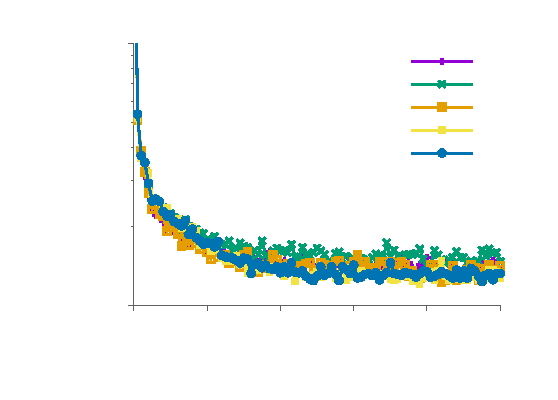
\includegraphics{chapter3/functionofepoch}}%
    \gplfronttext
  \end{picture}%
\endgroup

  \end{center}
  \caption{Evolution of the test error rate when learning MNIST using the square of a grid graph and for various normalizations, as a function of the epoch of training. The legend reads: ``l2'' means $\ell_2$ normalization of weights is used (with weights $10^{-5}$), ``Pos'' means parameters in $S$ are forced to being positive, and ``Norm'' means that the $\ell_1$ norm of each vector in the third dimension of $S$ is forced to 1.}
  \label{functionofepoch}
\end{figure}

\subsection{Experiments with covariance graphs}

As underlying graph structure, we use a thresholded covariance matrix obtained by using all the training examples. We choose the threshold so that the number of remaining edges corresponds to a certain density $p$ (5x5 convolutions correspond approximately to a density of $p=3\%$). We also infer a graph based on the $k$ nearest neighbors of the inverse of the values of this covariance matrix ($k$-NN). The latter two are using no prior about the signal underlying structure. The pixels of the input images are shuffled and the same re-ordering of the pixels is used for every image. Dimension of the first rank of $S$ is chosen equal to $k$ and its weights are initialized random uniformly.
GCTs are also compared with models obtained when replacing the first layer by a fully connected or convolutional one. Architecture used is the same as in the previous section. Results are reported on table~\ref{covar}.

\begin{table}[H]
  \caption{Error rates when topology is unknown on scrambled MNIST.}
  \begin{center}
    \bgroup
    \def\arraystretch{1.5}%  1 is the default, change whatever you need
    \begin{tabular}{|c|c|c|c|}
      \hline
      MLP & Conv5x5 & Thresholded ($p=3\%$) & $k$-NN ($k=25$)\\
      \hline
      1.44\% & 1.39\% & 1.06\% & 0.96\%\\
      \hline
    \end{tabular}
    \egroup
  \end{center}
  \label{covar}
  \end{table}

We observe that GCTs outperform the CNN and the MLP on scrambled MNIST. This is remarkable because that suggests it has been able to exploit information about the underlying structure thanks to its underlying graph.

\subsection{Improved convolutions on shallow architectures}

On CIFAR-10 (see \secref{sec:datasets}), we made experiments on shallow CNN architectures and replaced convolutions by receptive graphs. We report results on a variant of AlexNet~\citep{krizhevsky2012imagenet} using little distortion on the input that we borrowed from a tutorial of tensorflow~\citep{tensorflow2015-whitepaper}.
%On Cifar10, we use a variant of the AlexNet architecture applied on inputs with little distortion~\cite{krizhevsky2012imagenet}, borrowed from a tutorial of tensorflow~\cite{tensorflow2015-whitepaper}.
It is composed of two 5x5 convolutional layers of 64 feature maps, with max pooling and local response normalization, followed by two fully connected layers of 384 and 192 neurons.
On CIFAR-10, training architectures that learn $S$ took about $2.5$ times longer.
%We switched each convolutional layer with receptive graph layers, but kept the pooling ones.
We compare two different graph supports: the one obtained by using the underlying graph of a regular 5x5 convolution, and the support of the square of the grid graph. Optimization is done with stochastic gradient descent on 375 epochs where $S$ is freezed on the 125 last ones. Circulant one-hot intialization is used. These are weak classifiers for CIFAR-10 but they are enough to analyse the usefulness of the proposed layer.
%Exploring deeper architectures is left for further work.
Experiments are run five times each. Means and standard deviations of accuracies are reported in table~\ref{cifar}. ``Pos'' means parameters in $S$ are forced to being positive, ``Norm'' means that the $\ell_1$ norm of each vector in the third dimension of $S$ is forced to 1, ``Both'' means both constraints are applied, and ``None'' means none are used.

\begin{table}[H]
  \caption{Accuracies (in \%) of shallow networks on CIFAR-10.}
  \begin{center}
    \bgroup
    \def\arraystretch{1.5}%  1 is the default, change whatever you need
    \begin{tabular}{|c|c|c|c|c|c|c|}
      \hline
      Support & Learn $S$ & None & Pos & Norm & Both\\
      \hline
      \hline
      Conv5x5 & No & / & / & / & $86.8 \pm 0.2$\\
      \hline
      Conv5x5 & Yes & $87.4 \pm 0.1$ & $87.1 \pm 0.2$ & $87.1 \pm 0.2$ & $87.2 \pm 0.3$\\
      \hline
      Grid$^2$ & Yes & $87.3 \pm 0.2$ & $87.3 \pm 0.1$ & $87.5 \pm 0.1$ & $87.4 \pm 0.1$\\
      \hline
    \end{tabular}
    \egroup
  \end{center}
  \label{cifar}
\end{table}

The GCTs are able to outperform the corresponding CNNs by a small by statistically significant amount in a shallow architecture.

Learning the scheme $S$ imply a memory overhead due to the increase in the number of weights of each layer, thus why we limited this experiments to shallow architectures. An example of strategy to extend this experiment to deeper architectures is to tie the schemes of each layer together, or to reuse a same scheme (previously learned) for all layers.

%\todo{take S, and reuse it on resnet}

\subsection{Learning $S$ for semi-supervised node classification}
\label{sec:lss}

\todo{describe experiments and our model}

  Comparison of:
  \begin{itemize}
   \item Graph Convolution Network (GCN, \cite{kipf2016semi}),
   \item Graph Attention Network (GAT, \cite{velickovic2017graph}),
   \item Topology Adaptative GCN (TAGCN,  \cite{du2017topology}),
   \item Addition of graph dropout to GCN (GCN*, from \secref{sec:gsexp}),
   \item Graph Contraction Network (GCT, this work).
  \end{itemize}

  \begin{table}[H]
  \begin{center}
    \bgroup
    \def\arraystretch{1.5}%  1 is the default, change whatever you need
    \begin{tabular}{|c|c|c|c|c|c|c|}
      \hline
      Dataset & MLP & GCN & GAT & TAGCN & GCN* & GCT\\
      \hline
      \hline
      Cora & $58.8 \pm 0.9$ & $81.8 \pm 0.9$ & $83.3 \pm 0.6$ & $82.9 \pm 0.7$ & $\mathbf{83.4} \pm 0.7$ & $83.3 \pm 0.7$\\
      \hline
      Citeseer & $56.7 \pm 1.1$ & $72.2 \pm 0.6$ & $72.1 \pm 0.6$ & $71.7 \pm 0.7$ & $72.5 \pm 0.8$ & $\mathbf{72.7} \pm 0.5$\\
      \hline
      Pubmed & $72.6 \pm 0.9$ & $79.0 \pm 0.5$ & $78.3 \pm 0.7$ & $78.9 \pm 0.5$ & $78.2 \pm 0.7$ & $\mathbf{79.2} \pm 0.4$\\
      \hline
    \end{tabular}
    \egroup
  \end{center}
  \caption{Mean accuracy (in \%) and standard deviation from 100 runs}
  \label{tab:lss}
  \end{table}

\todo{discussion of results}\newpage
 \section{Translation-convolutional neural networks}
%\section{Extending CNNs using EC symmetries on graph domains}

\subsection{Methodology}


Our method is based on~\cite{pasdeloup2017convolutional}, where the authors have introduced a way to infer a graph from training signals, then translations from the obtained graph to design ad-hoc CNNs. We extend this approach and design strided convolutions along graph downscaling, data augmentation and convolutions on downscaled graphs. \figref{fig:outline} depicts the proposed method.

\begin{figure}[h!p]
\begin{framed}
  Step 0 (optional): infer a graph (see \cite{pasdeloup2017convolutional})
  \begin{center}
    \begin{tikzpicture}[thick]
      \node at (0,0) {$\mathbf{x}_0$};
      \path[black!20!white, dashed]
      (0.5,0) edge (2.5,0);
      \path
      (0.75, 0) edge[blue] (0.75, 0.13)
      (1.25, 0) edge[blue] (1.25, 0.1)
      (1.75, 0) edge[red] (1.75, -0.1)
      (2.25, 0) edge[red] (2.25, -0.05);
      \node[fill, circle, inner sep = 1pt, blue] at (0.75, 0.13) {};
      \node[fill, circle, inner sep = 1pt, blue] at (1.25, 0.1) {};
      \node[fill, circle, inner sep = 1pt, red] at (1.75, -0.1) {};
      \node[fill, circle, inner sep = 1pt, red] at (2.25, -0.05) {};
      \node at (0,-0.25) {$\mathbf{x}_1$};
      \begin{scope}[yshift=-0.25cm]
        \path
        (0.75, 0) edge[blue] (0.75, 0.07)
        (1.25, 0) edge[blue] (1.25, 0.08)
        (1.75, 0) edge[red] (1.75, -0.08)
        (2.25, 0) edge[red] (2.25, -0.15);
        \node[fill, circle, inner sep = 1pt,blue] at (0.75, 0.07){};
        \node[fill, circle, inner sep = 1pt,blue] at (1.25, 0.08){};
        \node[fill, circle, inner sep = 1pt,red] at (1.75, -0.08){};
        \node[fill, circle, inner sep = 1pt,red] at (2.25, -0.15){};        
      \end{scope}

      \path[black!20!white, dashed]
      (0.5,-0.25) edge (2.5,-0.25);
      \node at (0,-0.5) {\vdots};
      \node at (0,-1) {$\mathbf{x}_m$};
      \begin{scope}[yshift=-1cm]
        \path
        (0.75, 0) edge[blue] (0.75, 0.12)
        (1.25, 0) edge[red] (1.25, -0.05)
        (1.75, 0) edge[red] (1.75, -0.03)
        (2.25, 0) edge[blue] (2.25, 0.08);
        \node[fill, circle, inner sep = 1pt, blue] at (0.75, 0.12){};
        \node[fill, circle, inner sep = 1pt, red] at (1.25, -0.05){};
        \node[fill, circle, inner sep = 1pt, red] at (1.75, -0.03){};
        \node[fill, circle, inner sep = 1pt, blue] at (2.25, 0.08){};        
      \end{scope}
      \node at (1.5,-0.5) {\vdots};
      \path[black!20!white, dashed]
      (0.5,-1) edge (2.5,-1);

      \node at (3.25, -0.5) {\huge{$\Rightarrow$}};

      \begin{scope}[xshift=4cm]
        \node[draw, circle](a) at (0,0) {1};
        \node[draw, circle](b) at (1.5,0) {2};
        \node[draw, circle](c) at (1.5,-1) {4};
        \node[draw, circle](d) at (0,-1) {3};
      \end{scope}
      \path
      (a) edge (b)
      edge (d)
      (b) edge (d)
      (c) edge (d);
    \end{tikzpicture}
  \end{center}
  
  Step 1: infer translations
  \begin{center}
    \begin{tikzpicture}[thick]      
      \begin{scope}[xshift=0cm]
        \node[draw, circle](a) at (0,0) {1};
        \node[draw, circle](b) at (1.5,0) {2};
        \node[draw, circle](c) at (1.5,-1) {4};
        \node[draw, circle](d) at (0,-1) {3};
      \end{scope}
      \path
      (a) edge (b)
      edge (d)
      (b) edge (d)
      (c) edge (d);
      \node at (2.75, -0.5) {\huge{$\Rightarrow$}};
      \begin{scope}[xshift=4cm, scale=0.5, yshift=0.5cm]
        \node[draw, inner sep=2pt, circle](a) at (0,0) {};
        \node[draw, inner sep=2pt, circle](b) at (1.5,0) {};
        \node[draw, inner sep=2pt, circle](c) at (1.5,-1) {};
        \node[draw, inner sep=2pt, circle](d) at (0,-1) {};
      \end{scope}
      \path[black!20!white]
      (a) edge (b)
      edge (d)
      (b) edge (d)
      (c) edge (d);
      \path[->,>=stealth']
      (a) edge (b)      
      (d) edge (c);
      \begin{scope}[xshift=4cm, scale=0.5, yshift=-1.5cm]
        \node[draw, inner sep=2pt, circle](a) at (0,0) {};
        \node[draw, inner sep=2pt, circle](b) at (1.5,0) {};
        \node[draw, inner sep=2pt, circle](c) at (1.5,-1) {};
        \node[draw, inner sep=2pt, circle](d) at (0,-1) {};
      \end{scope}
      \path[black!20!white]
      (a) edge (b)
      edge (d)
      (b) edge (d)
      (c) edge (d);
      \path[->,>=stealth']
      (b) edge (a)      
      (c) edge (d);
      \begin{scope}[xshift=5.5cm, scale=0.5, yshift=0.5cm]
        \node[draw, inner sep=2pt, circle](a) at (0,0) {};
        \node[draw, inner sep=2pt, circle](b) at (1.5,0) {};
        \node[draw, inner sep=2pt, circle](c) at (1.5,-1) {};
        \node[draw, inner sep=2pt, circle](d) at (0,-1) {};
      \end{scope}
      \path[black!20!white]
      (a) edge (b)
      edge (d)
      (b) edge (d)
      (c) edge (d);
      \path[->,>=stealth']
      (a) edge (d);
      \begin{scope}[xshift=5.5cm, scale=0.5, yshift=-1.5cm]
        \node[draw, inner sep=2pt, circle](a) at (0,0) {};
        \node[draw, inner sep=2pt, circle](b) at (1.5,0) {};
        \node[draw, inner sep=2pt, circle](c) at (1.5,-1) {};
        \node[draw, inner sep=2pt, circle](d) at (0,-1) {};
      \end{scope}
      \path[black!20!white]
      (a) edge (b)
      edge (d)
      (b) edge (d)
      (c) edge (d);
      \path[->,>=stealth']
      (d) edge (a);
    \end{tikzpicture}
  
  \end{center}
  
  Step 2: design convolution weight-sharing

  \begin{center}
    \begin{tikzpicture}[thick]      
      \begin{scope}[xshift=0cm, scale=0.75, yshift=0.5cm]
        \node[inner sep=2pt](w) at (-1.0,-0.5) {$w_1 \times$};
        \node[draw, inner sep=2pt, circle](a) at (0,0) {};
        \node[draw, inner sep=2pt, circle](b) at (1.5,0) {};
        \node[draw, inner sep=2pt, circle](c) at (1.5,-1) {};
        \node[draw, inner sep=2pt, circle](d) at (0,-1) {};       
      \end{scope}
      \path[black!20!white]
      (a) edge (b)
      edge (d)
      (b) edge (d)
      (c) edge (d);
      \path[->,>=stealth']
      (a) edge (b)      
      (d) edge (c);
      \begin{scope}[xshift=0cm, scale=0.75, yshift=-1.5cm]
        \node[inner sep=2pt](w) at (-1.0,-0.5) {+ $w_2 \times$};
        \node[draw, inner sep=2pt, circle](a) at (0,0) {};
        \node[draw, inner sep=2pt, circle](b) at (1.5,0) {};
        \node[draw, inner sep=2pt, circle](c) at (1.5,-1) {};
        \node[draw, inner sep=2pt, circle](d) at (0,-1) {};
      \end{scope}
      \path[black!20!white]
      (a) edge (b)
      edge (d)
      (b) edge (d)
      (c) edge (d);
      \path[->,>=stealth']
      (b) edge (a)      
      (c) edge (d);
      \begin{scope}[xshift=2.5cm, scale=0.75, yshift=0.5cm]
        \node[inner sep=2pt](w) at (-1.0,-0.5) {+ $w_3 \times$};
        \node[draw, inner sep=2pt, circle](a) at (0,0) {};
        \node[draw, inner sep=2pt, circle](b) at (1.5,0) {};
        \node[draw, inner sep=2pt, circle](c) at (1.5,-1) {};
        \node[draw, inner sep=2pt, circle](d) at (0,-1) {};
      \end{scope}
      \path[black!20!white]
      (a) edge (b)
      edge (d)
      (b) edge (d)
      (c) edge (d);
      \path[->,>=stealth']
      (a) edge (d);
      \begin{scope}[xshift=2.5cm, scale=0.75, yshift=-1.5cm]
        \node[inner sep=2pt](w) at (-1.0,-0.5) {+ $w_4 \times$};      
        \node[draw, inner sep=2pt, circle](a) at (0,0) {};
        \node[draw, inner sep=2pt, circle](b) at (1.5,0) {};
        \node[draw, inner sep=2pt, circle](c) at (1.5,-1) {};
        \node[draw, inner sep=2pt, circle](d) at (0,-1) {};
      \end{scope}
      \path[black!20!white]
      (a) edge (b)
      edge (d)
      (b) edge (d)
      (c) edge (d);
      \path[->,>=stealth']
      (d) edge (a);

      \begin{scope}[xshift=5.0cm, scale=0.75, yshift=-0.5cm]
        \node[inner sep=2pt](w) at (-1.0,-0.5) {+ $w_0 \times$};
        \node[draw, inner sep=2pt, circle](a) at (0,0) {};
        \node[draw, inner sep=2pt, circle](b) at (1.5,0) {};
        \node[draw, inner sep=2pt, circle](c) at (1.5,-1) {};
        \node[draw, inner sep=2pt, circle](d) at (0,-1) {};
      \end{scope}
      \path[black!20!white]
      (a) edge (b)
      edge (d)
      (b) edge (d)
      (c) edge (d);
      \path[]
      (a) edge [loop above] (a)
      (b) edge [loop above] (b)
      (c) edge [loop below] (c)
      (d) edge [loop below] (d);

    \end{tikzpicture}
  
  \end{center}
  
  Step 3: design data augmentation
  \begin{center}
    \begin{tikzpicture}[thick]      
      \begin{scope}[xshift=0cm]
        \node[draw, inner sep = 2pt, circle](a) at (0,0) {};
        \node[draw, inner sep = 2pt, circle](b) at (1.5,0) {};
        \node[draw, inner sep = 2pt, circle](c) at (1.5,-1) {};
        \node[draw, inner sep = 2pt, circle](d) at (0,-1) {};
        \path[]
        (0, 0) edge[blue] (0, 0.52)
        (1.5, 0) edge[blue] (1.5, 0.4)
        (0, -1) edge[red] (0, -1.4)
        (1.5, -1) edge[red] (1.5, -1.2);
        \node[fill, circle, inner sep = 1pt, blue] at (0, 0.52) {};
        \node[fill, circle, inner sep = 1pt, blue] at (1.5, 0.4) {};
        \node[fill, circle, inner sep = 1pt, red] at (0, -1.4) {};
        \node[fill, circle, inner sep = 1pt, red] at (1.5, -1.2) {};
      \end{scope}
      \node at (-0.5,-0.5) {$\mathbf{x}_0$};
      \path[black!20!white]
      (a) edge (b)
      edge (d)
      (b) edge (d)
      (c) edge (d);
      \node at (2.25, -0.5) {\huge{$\Rightarrow$}};
      \begin{scope}[xshift=3cm, scale=0.5, yshift=0.75cm]
        \node[draw, inner sep=2pt, circle](a) at (0,0) {};
        \node[draw, inner sep=2pt, circle](b) at (1.5,0) {};
        \node[draw, inner sep=2pt, circle](c) at (1.5,-1) {};
        \node[draw, inner sep=2pt, circle](d) at (0,-1) {};
      \end{scope}
      \path[black!20!white]
      (a) edge (b)
      edge (d)
      (b) edge (d)
      (c) edge (d);
      \path[->,>=stealth']
      (a) edge (b)      
      (d) edge (c);
      \begin{scope}[xshift=4.5cm, scale=0.5, yshift = 0.75cm]
        \node[draw, inner sep = 2pt, circle](a) at (0,0) {};
        \node[draw, inner sep = 2pt, circle](b) at (1.5,0) {};
        \node[draw, inner sep = 2pt, circle](c) at (1.5,-1) {};
        \node[draw, inner sep = 2pt, circle](d) at (0,-1) {};
        \path[]
        (1.5, 0) edge[blue] (1.5, 0.52)
        %% (1.5, 0) edge[blue] (1.5, 0.4)
        (1.5, -1) edge[red] (1.5, -1.4);
        %% (1.5, -1) edge[red] (1.5, -1.2);
        \node[fill, circle, inner sep = 1pt, blue] at (1.5, 0.52) {};
        %% \node[fill, circle, inner sep = 1pt, blue] at (1.5, 0.4);
        \node[fill, circle, inner sep = 1pt, red] at (1.5, -1.4) {};
        %% \node[fill, circle, inner sep = 1pt, red] at (1.5, -1.2);
        \path[black!20!white]
      (a) edge (b)
      edge (d)
      (b) edge (d)
      (c) edge (d);
      \end{scope}      
      \begin{scope}[xshift=3cm, scale=0.5, yshift=-1.75cm]
        \node[draw, inner sep=2pt, circle](a) at (0,0) {};
        \node[draw, inner sep=2pt, circle](b) at (1.5,0) {};
        \node[draw, inner sep=2pt, circle](c) at (1.5,-1) {};
        \node[draw, inner sep=2pt, circle](d) at (0,-1) {};
      \end{scope}
      \path[black!20!white]
      (a) edge (b)
      edge (d)
      (b) edge (d)
      (c) edge (d);
      \path[->,>=stealth']
      (b) edge (a)      
      (c) edge (d);
      \begin{scope}[xshift=4.5cm, scale=0.5, yshift=-1.75cm]
        \node[draw, inner sep = 2pt, circle](a) at (0,0) {};
        \node[draw, inner sep = 2pt, circle](b) at (1.5,0) {};
        \node[draw, inner sep = 2pt, circle](c) at (1.5,-1) {};
        \node[draw, inner sep = 2pt, circle](d) at (0,-1) {};
        \path[]
        %% (0, 0) edge[blue] (0, 0.52)
        (0, 0) edge[blue] (0, 0.4)
        %% (0, -1) edge[red] (0, -1.4)
        (0, -1) edge[red] (0, -1.2);
        %% \node[fill, circle, inner sep = 1pt, blue] at (0, 0.52);
        \node[fill, circle, inner sep = 1pt, blue] at (0, 0.4) {};
        %% \node[fill, circle, inner sep = 1pt, red] at (0, -1.4);
        \node[fill, circle, inner sep = 1pt, red] at (0, -1.2) {};
        \path[black!20!white]
      (a) edge (b)
      edge (d)
      (b) edge (d)
      (c) edge (d);
      \end{scope}
    \end{tikzpicture}
  
  \end{center}
  Step 4: design subsampling and convolution weight-sharing

  \begin{center}
    \begin{tikzpicture}[thick, scale=0.7]
      \tikzstyle{every node} = [inner sep = 3pt];
      \small{\begin{scope}[xshift=-0.5cm]
        \node[draw, circle](a) at (0,0) {1};
        \node[draw, circle](b) at (1.5,0) {2};
        \node[draw, circle](c) at (1.5,-1) {4};
        \node[draw, circle](d) at (0,-1) {3};
      \end{scope}
      \path
      (a) edge (b)
      edge (d)
      (b) edge (d)
      (c) edge (d);
      \node at (2, -0.5) {\huge{$\Rightarrow$}};
      \begin{scope}[xshift=3.25cm]
        \node[draw, circle](a) at (0,0) {1};
        \node[draw, circle, black!20!white](b) at (1.5,0) {2};
        \node[draw, circle](c) at (1.5,-1) {4};
        \node[draw, circle, black!20!white](d) at (0,-1) {3};
      \end{scope}
      \path
      (a) edge (c);
      \node at (6, -0.5) {\huge{$\Rightarrow$}};
      \begin{scope}[xshift=7.75cm, scale=0.4, yshift=0.5cm]
        \node[inner sep=1pt](w) at (-2.0,-0.5) {$w_0 \times$};
        \node[draw, inner sep=1.5pt, circle](a) at (0,0) {};
        \node[draw, inner sep=1.5pt, circle, black!20!white](b) at (1.5,0) {};
        \node[draw, inner sep=1.5pt, circle](c) at (1.5,-1) {};
        \node[draw, inner sep=1.5pt, circle, black!20!white](d) at (0,-1) {};
      \end{scope}
      \path[black!20!white]
      (a) edge (c);
      \path[]
      (a) edge [loop above] (a)
      (c) edge [loop below] (c);
      \begin{scope}[xshift=10cm, scale=0.4, yshift=0.5cm]
        \node[inner sep=1pt](w) at (-2.0,-0.5) {+ $w_1 \times$};
        \node[draw, inner sep=1.5pt, circle](a) at (0,0) {};
        \node[draw, inner sep=1.5pt, circle, black!20!white](b) at (1.5,0) {};
        \node[draw, inner sep=1.5pt, circle](c) at (1.5,-1) {};
        \node[draw, inner sep=1.5pt, circle, black!20!white](d) at (0,-1) {};
      \end{scope}
      \path[black!20!white]
      (a) edge (c);
      \path[]
      (c) edge [->,>=stealth'] (a);

      \begin{scope}[xshift=7.75cm, scale=0.4, yshift=-2.5cm]
        \node[inner sep=1pt](w) at (-2.0,-0.5) {+ $w_2 \times$};
        \node[draw, inner sep=1.5pt, circle](a) at (0,0) {};
        \node[draw, inner sep=1.5pt, circle, black!20!white](b) at (1.5,0) {};
        \node[draw, inner sep=1.5pt, circle](c) at (1.5,-1) {};
        \node[draw, inner sep=1.5pt, circle, black!20!white](d) at (0,-1) {};
      \end{scope}
      \path[black!20!white]
      (a) edge (c);
      \path[->,>=stealth']
      (a) edge [] (c);
  
      }
    \end{tikzpicture}
  
  \end{center}
  \end{framed}
  \caption{Outline of the proposed method}
  \label{fig:outline}
  \vspace{-.5cm}
\end{figure}

\subsection{Background}

Define a graph $G = \langle V, E \rangle$ with $V$ the set of vertices, and $E \subseteq\binom{V}{2}$ the set of edges. We suppose the graph is connected, as conversely the process can be applied to each connected component of $G$. We denote by $d$ the max degree of the graph and $n = |V|$ the number of vertices.

The authors of~\cite{pasdeloup2017convolutional} propose to inductively define translations as functions from vertices to vertices as follows:

\begin{definition}\textbf{Candidate-translation}\\
  A \emph{candidate-translation} is a function $\phi: U \to V$, where $U \subset V$ and such that:
  \begin{itemize}[noitemsep,nolistsep]
  \item $\phi$ is \emph{injective}:\\
  $\forall v,v' \in U, \phi(v) = \phi(v') \Rightarrow v = v',$
  \item $\phi$ is \emph{edge-constrained}:\\
  $\forall v \in U, (v,\phi(v)) \in E,$
  \item $\phi$ is \emph{strongly neighborhood-preserving}:\\
  $\forall v,v' \in U, (v,v')\in E \Leftrightarrow (\phi(v),\phi(v')) \in E.$
  \end{itemize}
\end{definition}

The cardinal $|V-U|$ is called the \emph{loss} of $\phi$.
Two candidate-translations $\phi$ and $\phi'$ are said to be \emph{aligned} if $\exists v\in U, \phi(v) = \phi'(v)$.
We define $N_r(v)$ as the set of vertices that are at most $r$-hop away from a vertex $v \in V$.\\

\begin{definition}\textbf{Translation}\\
  A \emph{translation} in a graph $G$ is a candidate-translation such that there is no aligned translation with a strictly smaller loss, or is the identity function.
\end{definition}

Note that if the graph is a 2D grid, obtained translations are exactly natural translations on images~\cite{GrePasViaGri201610}.\\

\begin{definition}\textbf{Local translation}\\
A \emph{local translation} of center $v \in V$ is a translation in the subgraph of $G$ induced by $N_2(v)$, that has $v$ in its definition domain.
\end{definition}

As local translations can't be used to design data augmentation and convolutions on downscaled graphs, we also design proxies to global translations.

\begin{definition}\textbf{Proxy-translations}\\
A family of \emph{proxy-translations} $(\psi_p)_{p=0,..\kappa-1}$ initialized by $v_0 \in V$ is defined algorithmically as follows:
\begin{enumerate}
\item We place an indexing kernel on $N_1(v_0) $ i.e.\\ $N_1(v_0) = \{v_0, v_1, ..., v_{\kappa-1}\}$ with $\forall p, \psi_p(v_0) = v_p$,
\item We move this kernel using each local translation $\phi$ of center $v_0$: $\forall p, \psi_p(\phi(v_0)) = \phi(v_p)$,
\item We repeat 2) from each new center reached until saturation. If a center is being reached again, we keep the indexing that minimizes the sum of losses of the local translations that has lead to it.
\end{enumerate}
\end{definition}

\subsection{Efficiently finding translations}
Finding translations is an NP-complete problem~\cite{pasdeloup2017translations}, such that for large graphs the method is not suitable. 
In order to break down complexity, the authors of~\cite{pasdeloup2017convolutional} propose to search for local translations. They also introduce approximate translations which we omit for the sake of simplicity, but the description would be similar. We describe in three steps how we efficiently find proxy-translations.

\paragraph{First step: finding local translations}

For each vertex $v \in G$, we identify all local translations using a bruteforce algorithm. This process requires finding all translations in all induced subgraphs. There are $n$ such subgraphs, each one contains at most $d$ local translations. Finding a translation can be performed by looking at all possible injections from 1-hop vertices around the central vertex to any vertex that is at most 2-hops away. We conclude that it requires at most $\mathcal{O}(nd d^{2(d+1)})$ elementary operations and is thus linear with the order of the graph. On the other hand, it suggests that sparsity of the graph is a key criterion in order to maintain the complexity reasonable.

\figref{fig:gridgraph} depicts an example of a grid graph and the induced subgraph around vertex $v_0$. \figref{fig:inducedtranslations} depicts all obtained translations in the induced subgraph.

\begin{figure}[h!p]
  \begin{center}
    \begin{tikzpicture}[thick, scale = 0.7]
      \tikzstyle{every node} = [inner sep = 2pt];
      \foreach \x in {0,...,5}{
        \foreach \y in {0,...,4}{
          \node [draw, circle, dashed, black!50] at (\x, \y/2) {};
        }
      }
      \foreach \x in {0,...,4}{
        \foreach \y in {0,...,4}{
          \path[-]
          (\x,\y/2) edge[dashed, black!50] (\x+1,\y/2);
        }
      }
      \foreach \x in {0,...,5}{
        \foreach \y in {0,...,3}{
          \path[-]
          (\x,\y/2) edge[dashed, black!50] (\x,\y/2 + 1/2);
        }
      }
      \foreach \x in {0,...,5}{
        \foreach \y in {0,...,4}{
          \node [draw = black!50, dashed, circle,fill=white] at (\x, \y/2) {};
        }
      }
      \node[fill=blue!20!white] at (3,1){};
      \node at (3.4,1.2){\textcolor{blue}{$v_0$}};
      \node(bb) [draw, circle] at (3, 0) {};
      \node(s) [draw, circle] at (3, 1) {};
      \node(b) [draw, circle] at (3, 0.5) {};
      \node(u) [draw, circle] at (3, 1.5) {};
      \node(uu) [draw, circle] at (3, 2) {};
      \node(l) [draw, circle] at (2, 1) {};
      \node(lb) [draw, circle] at (2, 0.5) {};
      \node(lu) [draw, circle] at (2, 1.5) {};
      \node(r) [draw, circle] at (4, 1) {};
      \node(rb) [draw, circle] at (4, 0.5) {};
      \node(ru) [draw, circle] at (4, 1.5) {};
      \node(ll) [draw, circle] at (1, 1) {};
      \node(rr) [draw, circle] at (5, 1) {};
      \path[]
      (s) edge (u)
      edge (l)
      edge (b)
      edge (r)
      (l) edge (ll)
      edge (lu)
      edge (lb)
      (r) edge (rr)
      edge (ru)
      edge (rb)
      (u) edge (uu)
      edge (lu)
      edge (ru)
      (b) edge (bb)
      edge (lb)
      edge (rb);
    \end{tikzpicture}
  \end{center}
  \caption{Grid graph (in dashed grey) and the subgraph induced by $N_2(v_0)$ (in black).}
  \label{fig:gridgraph}
\end{figure}
\begin{figure}[h!t]
  \begin{center}
    \begin{tikzpicture}[thick,scale=1.5]
      \begin{scope}[scale=1.0]
        \tikzstyle{every node} = [inner sep=2pt]
        \node[fill=black, circle] at (3,1){};
        \node(bb) [draw, circle] at (3, 0) {};
        \node(s) [draw, circle] at (3, 1) {};
        \node(b) [draw, circle] at (3, 0.5) {};
        \node(u) [draw, circle] at (3, 1.5) {};
        \node(uu) [draw, circle] at (3, 2) {};
        \node(l) [draw, circle] at (2.5, 1) {};
        \node(lb) [draw, circle] at (2.5, 0.5) {};
        \node(lu) [draw, circle] at (2.5, 1.5) {};
        \node(r) [draw, circle] at (3.5, 1) {};
        \node(rb) [draw, circle] at (3.5, 0.5) {};
        \node(ru) [draw, circle] at (3.5, 1.5) {};
        \node(ll) [draw, circle] at (2, 1) {};
        \node(rr) [draw, circle] at (4, 1) {};
        \path[black!50, dashed]
        (s) edge (u)
        edge (l)
        edge (b)
        edge (r)
        (l) edge (ll)
        edge (lu)
        edge (lb)
        (r) edge (rr)
        edge (ru)
        edge (rb)
        (u) edge (uu)
        edge (lu)
        edge (ru)
        (b) edge (bb)
        edge (lb)
        edge (rb);
        \path[->,>=stealth']
        (s) edge (r)
        (r) edge (rr)
        (u) edge (ru)
        (b) edge (rb)
        (l) edge (s)
        ;
      \end{scope}
      \begin{scope}[xshift=2cm,scale=1.0]
        \tikzstyle{every node} = [inner sep=2pt]
      \node[fill=black, circle] at (3,1){};
      \node(bb) [draw, circle] at (3, 0) {};
      \node(s) [draw, circle] at (3, 1) {};
      \node(b) [draw, circle] at (3, 0.5) {};
      \node(u) [draw, circle] at (3, 1.5) {};
      \node(uu) [draw, circle] at (3, 2) {};
      \node(l) [draw, circle] at (2.5, 1) {};
      \node(lb) [draw, circle] at (2.5, 0.5) {};
      \node(lu) [draw, circle] at (2.5, 1.5) {};
      \node(r) [draw, circle] at (3.5, 1) {};
      \node(rb) [draw, circle] at (3.5, 0.5) {};
      \node(ru) [draw, circle] at (3.5, 1.5) {};
      \node(ll) [draw, circle] at (2, 1) {};
      \node(rr) [draw, circle] at (4, 1) {};
      \path[black!50, dashed]
      (s) edge (u)
      edge (l)
      edge (b)
      edge (r)
      (l) edge (ll)
      edge (lu)
      edge (lb)
      (r) edge (rr)
      edge (ru)
      edge (rb)
      (u) edge (uu)
      edge (lu)
      edge (ru)
      (b) edge (bb)
      edge (lb)
      edge (rb);
      \path[->,>=stealth']
      (s) edge (l)
      (r) edge (s)
      (u) edge (lu)
      (b) edge (lb)
      (l) edge (ll)
      ;
      \end{scope}
      \begin{scope}[xshift=4cm, scale=1.0]
        \tikzstyle{every node} = [inner sep=2pt]
        \node[fill=black, circle] at (3,1){};
        \node(bb) [draw, circle] at (3, 0) {};
        \node(s) [draw, circle] at (3, 1) {};
        \node(b) [draw, circle] at (3, 0.5) {};
        \node(u) [draw, circle] at (3, 1.5) {};
        \node(uu) [draw, circle] at (3, 2) {};
        \node(l) [draw, circle] at (2.5, 1) {};
        \node(lb) [draw, circle] at (2.5, 0.5) {};
        \node(lu) [draw, circle] at (2.5, 1.5) {};
        \node(r) [draw, circle] at (3.5, 1) {};
        \node(rb) [draw, circle] at (3.5, 0.5) {};
        \node(ru) [draw, circle] at (3.5, 1.5) {};
        \node(ll) [draw, circle] at (2, 1) {};
        \node(rr) [draw, circle] at (4, 1) {};
        \path[black!50, dashed]
        (s) edge (u)
        edge (l)
        edge (b)
        edge (r)
        (l) edge (ll)
        edge (lu)
        edge (lb)
        (r) edge (rr)
        edge (ru)
        edge (rb)
        (u) edge (uu)
        edge (lu)
        edge (ru)
        (b) edge (bb)
        edge (lb)
        edge (rb);
        \path[->,>=stealth']
        (s) edge (u)
        (r) edge (ru)
        (u) edge (uu)
        (b) edge (s)
        (l) edge (lu)
        ;
      \end{scope}
      \begin{scope}[xshift=6cm, scale=1.0]
        \tikzstyle{every node} = [inner sep=2pt]
        \node[fill=black, circle] at (3,1){};
        \node(bb) [draw, circle] at (3, 0) {};
        \node(s) [draw, circle] at (3, 1) {};
        \node(b) [draw, circle] at (3, 0.5) {};
        \node(u) [draw, circle] at (3, 1.5) {};
        \node(uu) [draw, circle] at (3, 2) {};
        \node(l) [draw, circle] at (2.5, 1) {};
        \node(lb) [draw, circle] at (2.5, 0.5) {};
        \node(lu) [draw, circle] at (2.5, 1.5) {};
        \node(r) [draw, circle] at (3.5, 1) {};
        \node(rb) [draw, circle] at (3.5, 0.5) {};
        \node(ru) [draw, circle] at (3.5, 1.5) {};
        \node(ll) [draw, circle] at (2, 1) {};
        \node(rr) [draw, circle] at (4, 1) {};
        \path[black!50, dashed]
        (s) edge (u)
        edge (l)
        edge (b)
        edge (r)
        (l) edge (ll)
        edge (lu)
        edge (lb)
        (r) edge (rr)
        edge (ru)
        edge (rb)
        (u) edge (uu)
        edge (lu)
        edge (ru)
        (b) edge (bb)
        edge (lb)
        edge (rb);
        \path[->,>=stealth']
        (s) edge (b)
        (r) edge (rb)
        (u) edge (s)
        (b) edge (bb)
        (l) edge (lb)
        ;
      \end{scope}
    \end{tikzpicture}
  \end{center}
  \caption{Translations (black arrows) in the induced subgraph (dashed grey) around $v_0$ (filled in black) that contains $v_0$ and only some of its neighbors.}
  \label{fig:inducedtranslations}
\end{figure}


\paragraph{Second step: using local translations to move a small localized kernel around $G$}

Given an arbitrary\footnote{In practice we run several experiments while changing the initial vertex and keep the best obtained result.} vertex $v_0 \in V$, we place an indexing kernel on $N_1(v_0)$ i.e. $N_1(v_0) = \{v_0, v_1, ..., v_{\kappa-1}\}$. Then we move it using every local translations of center $v_0$, repeating this process for each center that is reached for the first time. We stop when the kernel has been moved everywhere in the graph. In case of multiple paths leading to the same destination, we keep the indexing that minimizes the sum of loss of the series of local translations. We henceforth obtain an indexing of at most $\kappa$ objects of $N_1(v)$ for every $v \in V$.

This process is depicted in \figref{fig:movekernel}. Since it requires moving the kernel everywhere, its complexity is $\mathcal{O}(n d^2)$.

\begin{figure}[h!t]
  \begin{center}
    \begin{tikzpicture}[thick]
      \begin{scope}[scale=0.8]
        \node at (-1,2) {a)};
        \foreach \x in {0,...,5}{
          \foreach \y in {0,...,4}{
            \node [draw, circle, dashed, black!50] at (\x, \y) {};
          }
        }
        \foreach \x in {0,...,4}{
          \foreach \y in {0,...,4}{
            \path[-]
            (\x,\y) edge[dashed, black!50] (\x+1,\y);
          }
        }
        \foreach \x in {0,...,5}{
          \foreach \y in {0,...,3}{
            \path[-]
            (\x,\y) edge[dashed, black!50] (\x,\y + 1);
          }
        }
        \foreach \x in {0,...,5}{
          \foreach \y in {0,...,4}{
            \node(\x\y) [draw = black!50, dashed, circle,fill=white] at (\x, \y) {};
          }
        }
        \node at (3,2){$v_0$};
        \node at (2,2){$v_1$};
        \node at (1,2){$v_2$};
        \node at (1,3){$v_3$};

        \node[draw = black, circle] at (3,2){};
        \node[draw = red, circle] at (2,2){};
        \node[draw = green!50!black, circle] at (4,2){};
        \node[draw = blue, circle] at (3,3){};
        \node[draw = purple, circle] at (3,1){};
      \end{scope}
      \begin{scope}[xshift=5cm, scale=0.8]
        \node at (-1,2) {b)};
        \foreach \x in {0,...,5}{
          \foreach \y in {0,...,4}{
            \node [draw, circle, dashed, black!50] at (\x, \y) {};
          }
        }
        \foreach \x in {0,...,4}{
          \foreach \y in {0,...,4}{
            \path[-]
            (\x,\y) edge[dashed, black!50] (\x+1,\y);
          }
        }
        \foreach \x in {0,...,5}{
          \foreach \y in {0,...,3}{
            \path[-]
            (\x,\y) edge[dashed, black!50] (\x,\y + 1);
          }
        }
        \foreach \x in {0,...,5}{
          \foreach \y in {0,...,4}{
            \node(\x\y) [draw = black!50, dashed, circle,fill=white] at (\x, \y) {};
          }
        }
        \node at (3,2){$v_0$};
        \node at (2,2){$v_1$};
        \node at (1,2){$v_2$};
        \node at (1,3){$v_3$};
        \draw
        (0.5,2) -- (3,4.5) -- (5.5,2) -- (3,-0.5) -- (0.5,2);
        \path[->,>=stealth']
        (31) edge (21)
        (32) edge (22)
        (33) edge (23)
        (42) edge (32)
        (22) edge (12);
        \node[draw = black, circle] at (2,2){};
        \node[draw = red, circle] at (1,2){};
        \node[draw = green!50!black, circle] at (3,2){};
        \node[draw = blue, circle] at (2,3){};
        \node[draw = purple, circle] at (2,1){};
      \end{scope}
      \begin{scope}[scale=0.8, yshift=-6cm]
        \node at (-1,2) {c)};
        \foreach \x in {0,...,5}{
          \foreach \y in {0,...,4}{
            \node [draw, circle, dashed, black!50] at (\x, \y) {};
          }
        }
        \foreach \x in {0,...,4}{
          \foreach \y in {0,...,4}{
            \path[-]
            (\x,\y) edge[dashed, black!50] (\x+1,\y);
          }
        }
        \foreach \x in {0,...,5}{
          \foreach \y in {0,...,3}{
            \path[-]
            (\x,\y) edge[dashed, black!50] (\x,\y + 1);
          }
        }
        \foreach \x in {0,...,5}{
          \foreach \y in {0,...,4}{
            \node(\x\y) [draw = black!50, dashed, circle,fill=white] at (\x, \y) {};
          }
        }
        \node at (3,2){$v_0$};
        \node at (2,2){$v_1$};
        \node at (1,2){$v_2$};
        \node at (1,3){$v_3$};
        \draw
        (-0.5,2) -- (2,4.5) -- (4.5,2) -- (2,-0.5) -- (-0.5,2);
        \path[->,>=stealth']
        (21) edge (11)
        (22) edge (12)
        (23) edge (13)
        (32) edge (22)
        (12) edge (02);
        \node[draw = black, circle] at (1,2){};
        \node[draw = red, circle] at (0,2){};
        \node[draw = green!50!black, circle] at (2,2){};
        \node[draw = blue, circle] at (1,3){};
        \node[draw = purple, circle] at (1,1){};
      \end{scope}
      
      \begin{scope}[xshift=5cm, scale=0.8,yshift=-6cm]
        \node at (-1,2) {d)};
        \foreach \x in {0,...,5}{
          \foreach \y in {0,...,4}{
            \node [draw, circle, dashed, black!50] at (\x, \y) {};
          }
        }
        \foreach \x in {0,...,4}{
          \foreach \y in {0,...,4}{
            \path[-]
            (\x,\y) edge[dashed, black!50] (\x+1,\y);
          }
        }
        \foreach \x in {0,...,5}{
          \foreach \y in {0,...,3}{
            \path[-]
            (\x,\y) edge[dashed, black!50] (\x,\y + 1);
          }
        }
        \foreach \x in {0,...,5}{
          \foreach \y in {0,...,4}{
            \node(\x\y) [draw = black!50, dashed, circle,fill=white] at (\x, \y) {};
          }
        }
        \node at (3,2){$v_0$};
        \node at (2,2){$v_1$};
        \node at (1,2){$v_2$};
        \node at (1,3){$v_3$};
        \draw
        (-1.5,2) -- (1,4.5) -- (3.5,2) -- (1,-0.5) -- (-1.5,2);
        \path[->,>=stealth']
        (11) edge (12)
        (12) edge (13)
        (13) edge (14)
        (22) edge (23)
        (02) edge (03);
        \node[draw = black, circle] at (1,3){};
        \node[draw = red, circle] at (0,3){};
        \node[draw = green!50!black, circle] at (2,3){};
        \node[draw = blue, circle] at (1,4){};
        \node[draw = purple, circle] at (1,2){};
      \end{scope}
    \end{tikzpicture}
  \end{center}
  \caption{Illustration of the translation of a small indexing kernel using translations in each induced subgraph. Kernel is initialized around $v_0$ (a), then moved left around $v_1$ (b) using the induced subgraph around $v_0$, then moved left again around $v_2$ (c) using the induced subgraph around $v_1$ then moved up around $v_3$ (d) using the induced subgraph around $v_2$. At the end of the process, the kernel has been localized around each vertex in the graph.}
  \label{fig:movekernel}
\end{figure}


\paragraph{Final step: identifying proxy-translations in $G$}

Finally, by looking at the indexings obtained in the previous step, we obtain a family of proxy-translations defined globally on $G$. More precisely, each index defines its own proxy-translation. Note that they are not translations because only the local properties have been propagated through the second step, so there can exist aligned candidates with smaller losses. Because of the constraint to keep the paths with the minimum sum of losses, they are good proxies to translations on $G$.

An illustration on a grid graph is given in \figref{fig:translations}. The complexity is $\mathcal{O}(nd)$. Overall, all three steps are linear in $n$.

\begin{figure}[h!t]
  \begin{center}
    \begin{tikzpicture}[thick,scale=1.6]
      \tikzstyle{every node} = [inner sep = 2pt];
      \begin{scope}
        \foreach \x in {0,...,5}{
          \foreach \y in {0,...,4}{
            \node(\x\y) [draw, circle, black] at (\x, \y/2) {};
          }
        }
        \foreach \x in {0,...,4}{
          \foreach \y in {0,...,4}{
            \pgfmathtruncatemacro{\nouveaux}{\x+1}
            \path[->,>=stealth']            
            (\x\y) edge[bend left, green!50!black] (\nouveaux\y);
          }
        }
        \foreach \x in {0,...,5}{
          \foreach \y in {0,...,3}{
            \pgfmathtruncatemacro{\nouveauy}{\y+1}
            \path[->,>=stealth']
            (\x\y) edge[bend left, blue] (\x\nouveauy);
          }
        }
        \foreach \x in {1,...,5}{
          \foreach \y in {0,...,4}{
            \pgfmathtruncatemacro{\nouveaux}{\x-1}
            \path[->,>=stealth']
            (\x\y) edge[bend left, red] (\nouveaux\y);
          }
        }
        \foreach \x in {0,...,5}{
          \foreach \y in {1,...,4}{
            \pgfmathtruncatemacro{\nouveauy}{\y-1}
            \path[->,>=stealth']
            (\x\y) edge[bend left, purple] (\x\nouveauy);
          }
        }
      \end{scope}
    \end{tikzpicture}
  \end{center}
  \caption{Proxy-translations in $G$ obtained after moving the small kernel around each vertex. Each color corresponds to one translation.}
  \label{fig:translations}
\end{figure}

\subsection{Translation-convolution}

Let $(\psi_p)_{p=0,..,\kappa-1}$ be the proxy-translations identified on $G$ with the convention that $\psi_0 = id$ is the identity function, and where $\kappa$ is the number of weights in the indexing kernel.

The operation of the \emph{extended convolution layer} centered on the vertex $v \in V$ is defined as:

$$\mathbf{y}_v = h\left(\sum_{p=0}^{\kappa-1}{w_p \mathbf{x}_{\phi_p(v)}} + b\right)$$

where $h$ is the activation function, $b$ is the bias term, $\mathbf{x}_\bot = 0$ and:
$$
\left\{
    \begin{array}{ll}
        \phi_p(v) = \psi_p(v) & \mbox{ if } \psi_p \mbox{ is defined on } v \\
        \phi_p(v) = \bot \notin V & \mbox{ else} \\
    \end{array}
\right..
$$

Note that we defined convolution layers using the formalism of proxy-translations, but they can also be defined using only the formalism of local translations~\cite{pasdeloup2017convolutional}.

%Discussion with chapter 2

\subsection{Subsampling}

Downscaling is a tricky part of the process because it supposes one can somehow regularly sample vectors. As a matter of fact, a nonregular sampling is likely to produce a highly irregular downscaled graph, on which looking for translations irremediably leads to poor accuracy, as we noticed in our experiments.% Instead, here we propose to use translations on $G$ to define the extended downscaling layers. They basically are obtained by masking vertices in the initial graph.

We rather define the translations of the strided graph using the previously found proxy-translations on $G$.\\

\noindent\textbf{First step: extended convolution with stride $r$}
%\subsubsection{First step: convolution with stride $r$}
%Here we define an extended convolution layer with stride $r$.

Given an arbitrary initial vertex $v_0 \in V$, the set of kept vertices $V_{\downarrow r}$ is defined inductively as follows:
\begin{itemize}[noitemsep,nolistsep]
\item $V_{\downarrow r}^0 = \{v_0\}$,
\item $\forall t \in \mathbb{N}, V_{\downarrow r}^{t+1} = V_{\downarrow r}^t \cup \{v \in V, \forall v' \in V_{\downarrow }^t, v \not\in N_{r-1}(v') \land \exists v' \in V_{\downarrow r}^t, v \in N_{r}(v') \}$.
\end{itemize}

This sequence is nondecreasing and bounded by $V$, so it eventually becomes stationary and we obtain $V_{\downarrow r} = \lim_t{V_{\downarrow r}^t}$. Figure~\ref{downscaling} illustrate the first downscaling $V_{\downarrow 2}$ on a grid graph. %% $V_{\downarrow 2}$ is used to define the stride in extended convolution layers.

The output neurons of the extended convolution layer with stride $r$ are $V_{\downarrow r}$.

\paragraph{Second step: convolutions for the strided graph}

Using the proxy-translations on $G$, we move a localized $r$-hop indexing kernel over $G$. At each location, we associate the vertices of $V_{\downarrow r}$ with indices of the kernel, thus obtaining what we define as induced $_{\downarrow r}$-translations on the set $V_{\downarrow r}$. In other words, when the kernel is centered on $v_0$, if $v_1 \in V_{\downarrow r}$ is associated with the index $p_0$, we obtain $\phi_{p_0}^{\downarrow r}(v_0) = v_1$. Subsequent convolutions at lower scales are defined using these induced $_{\downarrow r}$-translations similarly to Subsection C.
%The downstream convolution's weight-sharing schemes are then obtained by moving a kernel covering the full graph to each vertex in $V_{\downarrow r}$, similarly to Subsection C.

%% Note that every downscaling layers of the extended architecture are defined from the translation found on the graph at the input level of the network. A typical extended CNN architecture would contain ${2^r}$ downscaled layers.

\begin{figure}[h!t]
  \begin{center}
    \begin{tikzpicture}[thick, scale=1.6]
      \tikzstyle{every node} = [inner sep = 2pt];
      \foreach \x in {0,...,5}{
        \foreach \y in {0,...,4}{
          \node [draw, circle, black!50] at (\x, \y/2) {};
        }
      }
      \foreach \x in {0,...,4}{
        \foreach \y in {0,...,4}{
          \path[-]
          (\x,\y/2) edge[black!50] (\x+1,\y/2);
        }
      }
      \foreach \x in {0,...,5}{
        \foreach \y in {0,...,3}{
          \path[-]
          (\x,\y/2) edge[black!50] (\x,\y/2 + 1/2);
        }
      }
      \foreach \x in {0,...,5}{
        \foreach \y in {0,...,4}{
          \pgfmathtruncatemacro{\sum}{\x+\y}
          \ifodd\sum
          \node(\x\y) [draw = black!50, circle,fill=white] at (\x, \y/2) {};
          \else
          \node(\x\y) [draw = black!50, circle,fill=black] at (\x, \y/2) {};
          \fi
        }
      }
      \node at (3.4,1.2){\textcolor{blue}{$v_0$}};
      \node[fill=blue!20!white] at (3,1){};
    \end{tikzpicture}
  \end{center}
  
  \caption{Downscaling of the grid graph. Disregarded vertices are filled in.}
  \label{fig:downscaling}
\end{figure}

\subsection{Data augmentation}

Once translations are obtained on $G$, one can use them to move training vectors, artificially creating new ones. Note that this type of data-augmentation is poorer than for images since no flipping, scaling or rotations are used.

\subsection{Matching CNNs on image classification}

On the CIFAR-10 dataset, our models are based on a variant of a deep residual network, namely PreActResNet18\cite{he2016identity}. We tested different combinations of graph support and data augmentation. For the graph support, we use either a regular 2D grid or either an inferred graph obtained by keeping the four neighbours that covary the most. \tabref{tab:cifar-table} summarizes out results. In particular, it is interesting to note that results obtained without any structure prior (91.07\%) are only 2.7\% away from the baseline using classical CNNs on images (93.80\%). This gap is even smaller (less than 1\%) when using the grid prior. Also, without priors our method significantly outperforms the others. %% In the top left corner of the table we fully exploit the fact that the dataset is composed of 2D structured data, and in the bottom right corner this information is not used at all. Even with that disadvantage, the results differ of only 2.7\%, which shows the strenght of the method when compared to others.

\begin{table}
\begin{center}
\caption{CIFAR-10 result comparison table.}
\vspace{-0.4cm}
\label{tab:cifar-table}
\resizebox{\columnwidth}{!}{%
\begin{tabular}{|l|c|c|c|c|c|c|}
\hline
\multirow{2}{*}{Support} & \multirow{2}{*}{\begin{tabular}[c]{@{}c@{}}MLP \\ \cite{LinMK15}\end{tabular}} & \multirow{2}{*}{CNN} & \multicolumn{2}{c|}{Grid Graph (Given)}       & \multicolumn{2}{c|}{Covariance Graph (Inferred)}         \\ \cline{4-7} 
                         &                                                                                &                      & \cite{defferrard2016convolutional} & Proposed & Proposed             & \cite{pasdeloup2017convolutional} \\ \hline
Full Data Augmentation   & 78.62\%                                                                        & \textbf{93.80\%}     & 85.13\%                            & 93.94\%  & 92.57\%              & ------                            \\ \hline
Data Augmentation - Flip & ------                                                                         & 92.73\%              & 84.41\%                            & 92.94\%  & 91.29\%              & ------                            \\ \hline
Graph Data Augmentation  & ------                                                                         & 92.10\%$^a$          & ------                             & 92.81\%  & \textbf{91.07\%}$^b$ & ------                            \\ \hline
None                     & 69.62\%                                                                        & 87.78\%              & ------                             & 88.83\%  & 85.88\%$^b$           & 82.52\%                           \\ \hline
\end{tabular}

}
\vspace{-0.2cm}
\end{center}
\footnotesize{$^a$ As the CNN does not have a graph support we used the covariance graph as support for the graph data augmentation.\\ $^b$ No priors about the structure}\\
\vspace{-.6cm}
\end{table}

\subsection{Experiments on fmri datasets}

The PINES dataset consists of fMRI scans on 182 subjects, during an emotional picture rating task\cite{chang2015sensitive}. We fetched individual first-level statistical maps (beta images) for the minimal and maximal ratings from \url{https://neurovault.org/collections/1964/}, to generate the dataset. Full brain data was masked on the MNI template and resampled to a 16mm cubic grid, in order to reduce dimensionality of the dataset while keeping a regular geometrical structure. Final volumes used for classification contain 369 signals for each subject and rating. 

We used a shallow network. The results on \tabref{tab:iaps-table} show that our method was able to improve over CNNs, MLPs and other graph-based extended convolutional neural networks.

\begin{table}[h]
\centering
\caption{PINES fMRI dataset accuracy comparison table.}
\label{tab:iaps-table}
\begin{tabular}{|l||c|c||c|c|}
\hline
\multicolumn{1}{|l||}{Graph} & \multicolumn{2}{c||}{None} & \multicolumn{2}{c|}{Neighborhood Graph}     \\ \hline
Method                      & MLP & CNN (kernel 1x1)                                 & \cite{defferrard2016convolutional} & Proposed                   \\ \hline
Accuracy                    & 82.62\% & 84.30\%                            & 82.80\%                            & \textbf{85.08\%} \\ \hline
\end{tabular}
\vspace{-.4cm}
\end{table}

\newpage
 %\section{Conclusion}
\label{sec:3.5}

In this chapter, we developped a new perspective to look at neural networks. This led us to discover that neural layers can be formulated with a ternary operation, that we called \emph{neural contraction}, between an input signal $X$, a weight kernel $\Theta$, and a weight sharing sheme $S$. We studied this representation and proposed efficient implementations. We saw it can represent any kind of layer. In particular we showed how related works from the literature can be represented with neural contractions. Also, we used it see the influence of symmetries, and concluded on their critical role in the success of convolutions. Then, we tested models on the task of graph signals classification and on the task of semi-supervised classification of nodes. To construct the scheme $S$, we tested ideas based on randomizations, from which we derived what we called \emph{Monte-Carlo Neural Networks} (MCNN), and a technique we called \emph{graph dropout}. We also tested to learn the scheme $S$, obtaining \emph{Graph Contraction Networks} (GCT). Finally, we tested to infer the scheme $S$ from a set of translations inferred from the domain, which we called \emph{Translation-Convolution Neural Networks} (TCNN). On image and fmri datasets, GCTs and TCNNs obtained performances that match those of CNNs. On scrambled image datasets, TCNNs obtained almost the same performance as in the non-scrambled case, outperforming alternatives by a large margin. On text documents, MCNNs beat the other graph convolution alternative. On citation networks, GCTs set new state-of-the-art results, but by small margins that are not statistically significant.\newpage

%
% Chapter 4 ----> as a section in chapter 3 maybe, or as a motivation in the introduction
%

% \chapter{Industrial applications}
% \todo{}
% \vfill\minitoc\newpage

%
% Conclusion
%

\chapter*{Conclusion}\label{chp:ccl}
\addcontentsline{toc}{chapter}{\nameref{chp:ccl}}
In this manuscript, after a presentation of the fields of research, we developed a theory on convolution of graph signals, and proposed new models that extend deep learning to graph domains.

\vspace{0.2cm}

In \chapref{chap:2}, we formulated two constructions of convolutions of signals defined on a vertex set $V$, based on a group $\Gamma$ acting on $V$. The $\varphi$-convolution can be employed when $\Gamma$ and $V$ are in one-to-one correspondence via an equivariant map $\varphi$, while the $\M$-convolution is a more convenient formulation that can be employed when $\Gamma$ is abelian. We proved that the characterization by equivariance to $\Gamma$, inherited from group convolutions holds. Then we introduced two properties that bind these convolutions with the edge set $E$ : edge-constraint (EC) and locality-preservation (LP). In view of describing operators that are used in deep learning, we proposed formulations with kernels of smaller supports, and proved that the weight sharing property holds. We demonstrated that the existence of convolutions on a graph can be characterized by the existence of Cayley subgraphs. For some graphs, their Cayley subgraphs might not be well representative of their topology. Therefore, we suggested a few strategies and we extended the previous results with convolutions based on groupoids rather than on groups. We constructed two types of groupoids, from partial transformations and paths, and were able to extend the results but also with some limitations. With the first type of groupoid this almost amounted to partition the graph into Cayley subgraphs, whereas with the second one it included degenerated cases.

\vspace{0.2cm}

In \chapref{chap:3} we proposed a novel layer representation for extending CNN architectures to other input domains. This representation is based on a ternary operation that we called \emph{neural contraction}, from which we derived new models: \emph{Monte-Carlo Neural Networks} (MCNN), \emph{Graph Contraction Networks} (GCT), \emph{Translation-Convolutional Neural Networks} (TCNN); and a new technique: \emph{graph dropout}. We also showed how to represent related models from the literature with neural contractions. The MCNN is a first idea exploiting the neural contraction. Roughly speaking, it is based on randomizing the structure that is leveraged, then averaging. So we didn't expect much from it but it fared well on a text categorization task. The GCT is based on the idea of learning how the weights are shared while learning them. It set new state-of-the-art performances on the task of semi-supervised classification of nodes in citation networks, but outperforms only by a small margin that is not statistically significant. In particular, we also observed that using graph dropout also significantly improved the results of alternative models on this type of tasks. The TCNN relies on constructing a convolution based on graph translations. It set a new state-of-the-art on classification of scrambled images by a large margin, and performs well on a fMRI dataset which is structured by a graph resembling a grid graph.

\vspace{0.2cm}

We tested these models in two types of tasks: supervised classification of graph signals and semi-supervised classification of nodes. The first task is historically the one that gave visibility to CNNs. However, we do not know of a dataset with a very unusual graph structure that is well fitted for the first task, or if it exists, it might not be the best graph to describe the underlying structure. This is why is practice, experiments for the supervised task are done with graphs resembling grid graphs to some extent. This is not the case for the semi-supervised task.

\vspace{0.2cm}

In the end, both task can be abstracted to a more general one. For example, let us consider a dataset represented by a matrix $X$, of shape $B \times N$, where $B$ is the number of instances and $N$ is the number of features. The linear part of the GCN layer formulation $Y = A X \Theta$ exploits both a graph on the rows (that we saw can be learned with the GCT) and a complete graph on the columns. Thus this layer amounts to two half layers, a sparse and a dense one. This idea can be generalized given a dataset represented by a tensor $X$ of rank~$r$. The formulation would then be $Y = g(X, A_1, A_2, \ldots, A_r)$ where $g$~realizes every tensor contractions between $X$ and each $A_i$ along the corresponding ranks. In that case, the $A_i$ can be seen as a learnable normalized adjacency matrix corresponding to a graph structure on the $i\powth$ rank. This idea can originate a class of neural networks that can be called \emph{multiary neural networks}.

\vspace{0.2cm}

As pointed out in the introduction, this work participates in making CNNs more generic, and thus applicable to a broader range of real world problems. In the process, we also advanced our understanding of convolutions, providing a thorough description with a set of expressions, mathematical results and theorems about how to extend them on graph domains while preserving key properties, and how to characterize them. We hope that the reader had pleasure reading this manuscript and that it gave him ideas and shed new lights !%. Let us thrive for a continuous effort to help advance collectively the boundaries of human knowledge at our scales and beyond !

%
% Bibliography
%

\printbibliography[heading=bibintoc]

%
% Bin
%

% \setcounter{chapter}{-1}
% \chapter{Trash bin and more drafts}
% ... that we may use in some section.
% \vfill\minitoc\newpage

% \input{chapter_unsorted/disamb}\newpage
% % could be renamed: why not dense layers ?


\section{Expressivity analysis of dense versus sparse connectivity}

Let consider a tensor input $x$ of a neural network layer $l$. Without loss of generality, we consider that $x$ is a matrix of shape $n \times p$. Its rows are supposed structured by a graph $G = <V, E>$, with $|V| = n$, its columns are its feature maps.

In what follows, we discuss the expressivity and efficiency of a dense layer with $x$ as input versus a layer that would leverage $G$. We start with the regular case and continue onto non-regular structures.

\subsection{Strong regular case}

In the strong regular case, $G$ is a lattice graph such that a convolution is defined naturally on it. For example, this is the case where rows of $x$ defines ticks of a time series, or flattened pixels of an image.

Let consider a convolutional layer $c = (g_c,h_c)$ with padding, defined by $q$ filters of width $k$. Define $y_c$ its output of shape $n \times q$.

We are interested in knowing if there exists a dense layer that can efficiently replicate $c$.

Its connectivity matrix $W_c$ is of shape $np x nq$. Obviously, the function $g_c$ can be replicated by a dummy dense layer $d = (g_c,h_d)$ through $W_c$. However, whereas $c$ has only $kpq$ weights, $d$ has $n^2pq$. If we consider the families of neural networks $\cc$, $\cd$ spaned by their weights $\theta_c$, $\theta_d$, then we realize the $\cc$ is less expressive, but in the same time it is more efficient at representing its functions.

Let's define the notion of partial expressivity with respect to a family of functions.

Let $\cf$ a family of functions, $\cl$ a family of layer functions, and $\epsilon$ the approximation coefficient. For $f \in \cf$, define $S_{\epsilon}(\cl,f) = \{l \in \cl, d(l,f) < \epsilon \}$ and $S_{\epsilon}(\cl,\cf) = \displaystyle \bigcup_{f \in \cf} S_{\epsilon}(\cl,f)$.

\todo{reword above}

By abusing and anticipating future correction of this manuscript, we consider that $\cc$ and $\cd$ are vector spaces. We are interesting in 1. proving that $S_{\epsilon}(\cc,\cf)$ and $S_{\epsilon}(\cd,\cf)$ are also vector spaces, and 2. analysing for which $\cf$, $\frac{dim(S_{\epsilon}(\cc,\cf))}{dim(S_{\epsilon}(\cd,\cf))}$ is maximized.

Obviously 1. is false, so 2. is ill-posed (this draft is to be reworded afterward). Instead of using $dim$, we should rather use $card$. However they are potentially infinite families so we should rather use a notion of volume, except if we discretize. So let's discretize.

By the way, `'modified`' 2. is trivially maximized for $\cf = \cc$ (and then the ratio equals $1$), so let's weaken $\cf$ and say it's any family with translation equivariance. We are then interested in proving that if $\cf$ is the family on translation equivariant function (on this domains that has to be specified when rewriting this section), then $\frac{card(S_{\epsilon}(\cc,\cf))}{card(S_{\epsilon}(\cd,\cf))}$ is close to $1$. Equivariant in our context means commuting with translations (we should rather use the latter expression btw).

The result might be obtained without discretizing as convolutions with padding commutes with translations. Let's guess that they are close to other commuters. In fact that is even it. Proof with Fourier analysis.

% Let's discretize. We assume that entries of $x$ takes their values into a finite set $M = \{m_1, m_2, \ldots, m_r\}$.


% To unburden the notation, we'll assume $p=q=1$ and reshape to matrix-vector operations. A function $f \in \cf$ is defined by the values assigned to dimensions of $x$. For each $i \in \{1, 2, \ldots, n\}$, we define the grid tensor $\ca^f_i$, such that
% \begin{gather*}
% \forall j \in \{1, 2, \ldots, n\}, \forall i_j \in \{1, 2, \ldots, r\} \\
% \ca^f_i[i_1,i_2,\ldots,i_n] = f(x)[i] \Leftrightarrow \forall s \in \{1, 2, \ldots, n\}, x[s] = m_{i_s}
% \end{gather*}


\subsection{Draft}

The only dense layer that replicate $g_c$ is obtained through the connectivity matrix $W_c$. $\cd$ is more expressive, however less efficient as we are looking for equivariant functions. It happens that equivariant functions are exactly convolutions with padding.


\newpage
% \section{Conv drafts}


\todo{point}

In particular, we have
\begin{align*}
\forall s \in \cs(\Gamma), \widetilde\varphi(s) & = \widetilde\varphi\left( \displaystyle \sum_{g \in \Gamma} s[g] \delta_g \right)\\
& = \displaystyle \sum_{g \in \Gamma} s[g] \widetilde\varphi\left(\delta_g \right)\\
& = \displaystyle \sum_{g \in \Gamma} s[g] \delta_{\varphi(g)}\\
& = \displaystyle \sum_{v \in V} s[\varphi^{-1}(v)] \delta_{v}\\
\widetilde\varphi(s) & = \displaystyle \sum_{v \in V} \widetilde\varphi(s)[v] \delta_v\\
\end{align*}

So $\widetilde\varphi(s)[v] = s[\varphi^{-1}(v)]$ and $\widetilde\varphi(s)[\varphi(g)] = s[g]$. Let's simplify the notations with $\widetilde\varphi(s) = t$ and $\varphi(g) = v$, \ie $t[v] = s[g]$ as expected. We then define the group convolution on $\cs(V)$ as
\begin{align*}
(t_1 \ast t_2)[v] & = (s_1 \ast s_2)[g]\\
& = \displaystyle \sum_{h \in \group} s_1[h] \h{2} s_2[h^{-1}g]\\
& = \displaystyle \sum_{u \in V} s_1[\varphi^{-1}(u)] \h{2} h_u(s_2)[\varphi^{-1}(v)]\\
& = \displaystyle \sum_{u \in V} t_1[u] \h{2} \widetilde\varphi(h_u(s_2))[v]\\
\end{align*}



\begin{gather}
(t_1 \ast t_2)[v] = \displaystyle \sum_{u \in V} t_1[u] \h{2} h_u(t_2)[v]\\
\end{gather}


\todo{stop sign}




Recall that
\begin{align*}
\delta_{g}[h] & = \begin{cases} 1 & \text{if } h = g \Leftrightarrow \varphi(h) = \varphi(g)\\ 0 & \text{otherwise} \end{cases}\\
              & = \delta_{\varphi(g)}[\varphi(h)]
\end{align*}

\begin{align*}
s & = \displaystyle \sum_{v \in V} s[v] \h{2} \delta_v
\end{align*}






\todo{lemme on existence of uncountable linearly independent irrational family ?}

\begin{proposition} The group convolution on $\cs(\Gamma)$ has a unique neutral element which is the dirac signal on the identity tranformation.
\end{proposition}
\begin{proof}
Denote $\delta$ a neutral element for the group convolution. Note as because of the commutativity the group convolution, a left neutral element is also a right neutral element. We have $$s[h] = (\delta \ast s)[h] = \displaystyle \sum_{g \in \Gamma} \delta[g] \h{2} s[g^{-1}h]$$ which is true for any real valued signal. By chosing a signal $\pi$ having linearly independant irrational entries (and using the axiom of choice in case G is not finite), we obtain that $$\delta[g] = \begin{cases} 1 \text{ if } g = \id\\ 0 \text{ otherwise}\end{cases} \ie \quad \delta = \delta_{\id}$$
Conversely, $(\delta_{\id} \ast s)[h] = 1 . s[{\id}^{-1}h] = s[h]$.
\end{proof}











In other therms, if there is an isomorphism between $\Gamma$ and $V$, the group structure pass to $V$ as well as the definition of the group convolution.






To alleviate this issue, let's introduce the neutral elements $\delta$ of the convolution, and the neutral element $\id \in \Phi^*(V)$.


With the help of $\delta$, we follow the same process as in the proof of \propref{prop:equi}, see \eqref{eq:conv}, to construct the class of group convolutional operators which defines exactly the class of linear transformations that are equivariant to a certain group.


% \begin{definition}\textbf{Group convolution}\\



% \end{definition}








On graphs, this could be used provided we defined meaningful translations beforehand (see \secref{}). Another possibilty would be to search for invariances with respect to graph equivariances and derive a convolution operator similarly than for translations. This approach, which uses group convolutions~\citep{weinstein1996groupoids}, has already been discussed on regular domain to extend CNNs to other invariances than translational ones~\citep{cohen2016group,hoogeboom2018hexaconv}, as well as on spherical domain with rotation equivariant CNNs~\citep{cohen2018spherical}. As stated from the previous remark, the big advantage of this approach is that there is no loss of expressivity. However on graphs, this would be more challenging as it's not likely there exists transformations with equivariances. However, let's suppose we found such a set of transformations on a graph, then for \propref{prop:equi} to hold (instead as for regular translations), we see in the proof that they need to be bijective \eqref{eq:bij} and vertex dependent \ref{eq:conv}.




\subsection{}



\begin{definition}\textbf{Grounded set of transformations}\\
A set of transformations over a graph $\gve$, \emph{grounded} on a vertex $v_0 \in V$, denoted $\cp_{v_0} \subset \Phi(V)$, is a set that is in one-to-one correspondence with $V$, such that $\forall v \in V, \exists! p_v \in \cp_{v_0}, p_v(v_0) = v$.
\end{definition}

We have $\cp_{v_0} = \order(G) \in \bbn \cup \{+\infty\}$. For notational convenience we drop the subscript $_{v_0}$ in what follows.

\begin{definition}\textbf{$\cp$-equivariant convolution operator}\\
Let $\gve$ a graph, not necessarily a grid. Let $\cp$ a grounded set of transformations. Then, the  $\cp$-equivariant convolution operator $f_w$ is defined as
\begin{gather*}
\forall s \in \cs(V), f_w(s) = s \ast_{\cp} w = \displaystyle \sum_v s[v] \h{2} p_v(w)
\end{gather*}
\end{definition}

\begin{claim}\textbf{Characterization of $\cp$-eq. convolution operator}\\
The class of linear graph signal transformations that are equivariant to a grounded set $\cp$ is exactly the class of $\cp$-equivariant convolutive operations.
\end{claim}

\begin{proof}
By construction of $\cp$-equivariant convolutions, the proof is similar to the one of \propref{prop:equi}.
\end{proof}


\newpage
% \section{Conv graph Draft}

\subsection{Construction on Cayley graphs}

Let's suppose that from a vertex set $V$, we have constructed a convolution of the form $*_{\III}$, with $\Gamma \overset{\varphi}{\equiv} V$. One particular underlying graph structure would be define as the digraph $\vgve$, with $E=\{ (u,v), \exists g \in \Gamma, g(u) = v \}$. However, such graph would just be the complete digraph. To keep the information about the group $\Gamma$ somehow in $E$, without obtaining a complete digraph, we need to at least consider a generating set $\cu$. Hence, it is enough to define the edge set as $E=\{ (u,v), \exists g \in \cu, g(u) = v \}$. Conversely, an edge set $E$ with these hypotheses would then naturally support a graph convolution. This leads us to study the particular class of Cayley graphs~\citep{cayley1878desiderata,wiki:cayley}.

We now consider the class of Cayley (di)graphs~\citep{cayley1878desiderata,wiki:cayley} because the $\varphi$-equivalence property \eqref{eq:P} naturally holds on them.
\todo{rewrite and obtain: On a Cayley graph, there is $\varphi$ such that the subgroupoid of transformation that are EC is $\varphi$-equivalent (proof on $\cu$ then extended)}

\begin{definition}\textbf{Cayley graph}\\
Let a group $\Gamma$ and one of its generating set $\cu$. The \emph{Cayley graph} generated by $\cu$, is the digraph $\vgve$ such that $\Gamma \overset{\varphi}{\equiv} V$ and $E$ is such that:
\begin{gather*}
a \sim b \Leftrightarrow \exists u \in \varphi(\cu) \subset V, g_u(a) = b
\end{gather*}
\end{definition}

Cayley graphs allows to alleviate \ref{itm:d1} by summing onto the generating set~$\cu$ instead of onto~$\Gamma$.%, which also makes the convolution on Cayley graphs edge-constrained.

\begin{definition}\textbf{Cayley graph convolution}\\
\begin{align*}
\forall u \in V, (s_1 \ast_{\C} s_2) [u] & = \displaystyle \sum_{g \in \cu} s_1[g] \h{2} g(s_2)
\end{align*}
\end{definition}

Conversely, let a graph $\gve$ and a $\varphi$-equivalent subgroup $\Gamma \subseteq \Phi^{*}(V)$. Then we can generate a Cayley graphs with a generating set of $\Gamma$, and thus define a Cayley graph convolution. In particular, when transformations of~$\Gamma$ are edge-constrained, that would also be the case for this convolution on $G$, which leads us to study edge-constrained transformations.

\todo{operator and characterization}
\todo{which graph is a Cayley graph ?}

\subsection{Construction on graph groupoids}

% need abelian for path commutation. But can choose to take minimal path related to some choice. Cf bastnet.

\todo{work in progress}

On graphs, we notice that the property \eqref{eq:P} can be realized by transformations acting on edges. However, unless the graph is complete, these actions can't be composed everywhere to form another edge constrained action. The algebraic structure that posesses the same kind of properties than a group except that its composition law is not defined everywhere is called a groupoid. The following definitions clarify our discussion.

\begin{definition}\textbf{Groupoid}\\
A groupoid is a set equiped with a closed partial composition law, a unique identity element, and every unique inverses.
\end{definition}

\begin{remark}We use the convention than left and right inverses must be the same.
\end{remark}

\begin{definition}\textbf{Graph groupoid}\\
The \emph{groupoid} $\cp(G)$ of a graph $\gve$ is the set of its paths equiped with:
\begin{enumerate}
\item two maps $\psi$ and $\varphi$ that respectively map a path to its first and last element,
\item a closed partial composition law $gh$ defined if and only if $\psi(g) = \varphi(h)$, which concatenates $g$ behind $h$ and \sout{removes adjacent duplicate vertices} \textcolor{red}{to rewrite},
\item an inverse operator $\h{0}^{-1}$ which maps a path to its reverse,
\item an identity element $\id$ which is the path of length $0$.
\end{enumerate}
\end{definition}

\begin{remark}Recall from \defref{def:path} that a path can't contain adjacent duplicates.
\end{remark}

\begin{remark}Note that even though the composite path $gh$ has elements of $h$ before those of $g$ we write $gh$ instead of $hg$ because we'll need the left operand to act on the right one through functional notation $g(h)$.
\end{remark}

\begin{definition}\textbf{Graph $k$-groupoid}\\
The \emph{$k$-groupoid} $\cp_k(G)$ of a graph $\gve$, for $k \in \bbn^*$, is the groupoid obtained by restricting $\cp(G)$ to paths of length at most $k$ (the definition domain of its composition law is also further restricted by the length of the resulting paths in $\cp(G)$).
\end{definition}

\begin{definition}\textbf{$k$-Groupoid convolution}\\
Let a graph $\gve$. Let a subgroupoid $\Gamma \subseteq \cp_k(G)$. The $k$-groupoid convolution between two signals $s_1$ and $s_2 \in \cs(\Gamma)$ is defined as:
\begin{align*}
\forall h \in \Gamma, (s_1 \ast s_2) [h] & = \displaystyle \sum_{\substack{(a,b) \in \Gamma^2 \\ \st ab=h }} s_1[a] \h{2} s_2[b] \\
& = \displaystyle \sum_{\substack{g \in \Gamma\\ \st \varphi(g) = \varphi(h)}} s_1[g] \h{2} s_2[g^{-1}h]\\
& = \displaystyle \sum_{\substack{g \in \Gamma\\ \st \psi(g) = \psi(h)}} s_1[hg^{-1}] \h{2} s_2[g]
\end{align*}
\label{def:pconv}
\end{definition}

\begin{claim}\textbf{Path transformation}\\
Let a graph $\gve$. By identifying vertices with paths of length $1$, a path $g \in \cp(G)$ can act as a transformation on $v \in V$ through the composition law of $\cp(G)$. Also note that $g(v) = g(v^{-1})$.
\end{claim}

We can nom define the $k$-Groupoid convolution operator on $\cs(G)$ by restriction of the second operand from $\cs(\Gamma)$ to paths of length $1$:

\begin{definition}\textbf{$k$-Groupoid convolution operator}\\
Let a graph $\gve$. Let a subgroupoid $\Gamma \subseteq \cp_k(G)$. The $k$-groupoid convolution operator $f_w$ with parameter $w \in \cs(\Gamma)$ is defined as:
\begin{gather*}
\forall s \in \cs(\Gamma), \forall h \in \Gamma, f_w(s)[h] = (s \ast w)[h]
\end{gather*}
And when restricted to $\cs(G)$ it is defined as:
\begin{gather*}
\forall s \in \cs(G), \forall v \in V, f_w(s)[v] = \displaystyle \sum_{\substack{g \in \Gamma\\ \st \psi(g) = v}} s[g(v)] \h{2} w[g]\\
\forall s \in \cs(G), \forall v \in V, f_w(s)[v] = \displaystyle \sum_{\substack{g \in \Gamma\\ \st \varphi(g) = v}} s[g] \h{2} w[g^{-1}(v)]
\end{gather*}
\end{definition}

\begin{proposition}\textbf{Groupoid equivariance to $\Gamma$}\\
$k$-Groupoid convolution operators on $\cs(G)$ are groupoid equivariant to $\Gamma$ \ie
\begin{gather*}
\exists w \in \cs(\Gamma), f = w \ast . \Rightarrow
\forall v \in V, \forall g \in \Gamma \st \psi(g^{-1}) = v,
f \circ g [v]= g \circ f [v]
\end{gather*}
\end{proposition}

\begin{gather}
g(h(v)) maybe false
\end{gather}


Mini patron of todo:
\begin{itemize}
\item Equivariance to $\Gamma$ holds, proof
\item Converse of characterization does not hold yet, except on orbits
\item property for it to hold
\item relaxing one-to-one correspondence constraint but keeping other properties
\item other avenue instead of property: should make use of edges to build a group structure
\item ideal graph (lattice-regular)
\item if group is too much then just groupoid structure from edges is enough
\end{itemize}

\todo{finish this section}

\subsection{To rename}

% \begin{definition}\textbf{Infinite graph}\\
% An \emph{infinite graph} is defined by natural extension of the notion of graph $G=\langle V,E \rangle$ where $V$ and $E$ can be infinite. We denote $\order{G} = \infty$.
% \end{definition}

\begin{definition}\textbf{Graph automorphisms}\\
A graph automorphism of a graph $\gve$ is a bijection in the vertex domain $\phi: V \rightarrow V$ such that $\{u,v\} \in E \Leftrightarrow \{\phi(u), \phi(v)\} \in E$. We denote $\ca(G)$ the group of automorphism on $G$.

We denote by $\ce(\phi)$ the set of input-output mapping of $\phi$, defined as $\ce(\phi) = \{ (x,y) \in V^2, \phi(x) = y \}$.

A graph automorphism $\phi$ is said to be \emph{edge-constrained} (EC) if $\ce(\phi) \subseteq E$. We denote $\ca_{\EC}(G)$ the set of edge-constrained automorphism on $G$.
\end{definition}

\begin{definition}\textbf{Orthogonality}\\
Two graph automorphisms $\phi_1$ and $\phi_2$ are said to be orthogonal, if and only if $\ce(\phi_1) \cap \ce(\phi_2) = \emptyset$, denoted $\phi_1 \bot \phi_2$. They are said to be aligned otherwise.

Similarly, we define orthogonality of $r$ automophisms as $\phi_1 \bot \cdots \bot \phi_r \Leftrightarrow \ce(\phi_1) \cap \cdots \cap \ce(\phi_r) = \emptyset$
\end{definition}


\subsection{Lattice-regular graph}

\begin{definition}\textbf{Lattice-regular graph}\\
A lattice-regular graph is a regular graph that admits $r$ orthogonal edge-constrained automorphisms, where $r$ is its degree.
\end{definition}


%\subsubsection{Grids}{}

%\subsubsection{Lattices}

%\subsubsection{Spatial graphs}

%\subsubsection{Projections of spatial graphs}\newpage

%
% Post body
%

% % Temptative previsional plan
% \setcounter{chapter}{-1}
% \fakechapter{Temptative previsional plans}
% \includepdf[pages=1-7]{others/temptative_plan.pdf}

% % keywords and temptative titles
% \setcounter{chapter}{-1}
% \chapter{Keywords and temptative titles}
% \begin{keywords}
Deep learning,
representation learning,
propagation learning,
visualization,
structured,
unstructured regular,
irregular,
covariant,
invariant,
equivariant,
tensor,
scheme,
weight sharing,
graphs,
manifold,
euclidean,
signal processing,
graph signal processing,
time series,
time series database,
distributed application,
spatial-time series,
geo time series,
industrial applications,
warp 10,
warpscript,
...
\end{keywords} % to be put somewhere else
% \section*{Temptative titles}

\begin{itemize}
\item Learning propagational representations of irregular and unstructured data
\item Learning representations of unstructured or irregularly structured datasets
\item Propagational learning of unstructured or irregularly structured datasets
\item Learning tensorial representation of irregular and unstructured data
\item Tensorial representation of propagation in deep learning for irregular and unstructured dataset
\item Structural representation learning for irregular or unstructured data
\item Word for both ``irregularly structured'' + ``unstructured'' = ? (maybe ``unorthodox'' ?)
\item Unorthdox deep learning
\item ...
\item Deep learning of unstructured or irregularly structured datasets
\item Deep learning models for data without a regular structure
\item On structures in deep learning
\item On deep learning for when data is lacking a regular structure
\item Deep learning for non regularly structured data
\end{itemize}


\end{document}